\documentclass{article}

%\usepackage[paperheight=16cm,paperwidth=14cm,textwidth=12cm]{geometry}
% Load blindtext package for dummy text
\usepackage{parskip}

\usepackage[ mincrossrefs=999, style=numeric, backend=biber, url=false,
isbn=false, doi=false, ]{biblatex}

\addbibresource{references.bib}

\usepackage[margin=1in]{geometry}

\usepackage{fontspec}
\usepackage{fullpage}

\usepackage[colorlinks]{hyperref}
\usepackage{enumitem}
\usepackage{agda}



\usepackage{unicode-math}
\usepackage{stmaryrd}
\usepackage{amsfonts}
\usepackage{mathtools}
\usepackage{xspace}

\setlist[itemize]{noitemsep, topsep=0pt}
%\hypersetup{ citecolor=RoyalBlue }
\usepackage{tikz-cd}
\usepackage{titlesec}
%\titlespacing\section{0pt}{4pt plus 2pt minus 2pt}{4pt plus 2pt minus 2pt}
\usepackage{graphicx} % for images
\usepackage{float} % for figure[H]



\setmainfont{DejaVu Serif}
\setsansfont{DejaVu Sans}
\setmonofont{DejaVu Sans Mono}

% \setmonofont{Fira Mono}
% \setsansfont{Noto Sans}



\usepackage{xcolor}
\definecolor{asparagus}{rgb}{0.53, 0.66, 0.42}
\definecolor{applegreen}{rgb}{0.55, 0.71, 0.0}
\definecolor{armygreen}{rgb}{0.29, 0.33, 0.13}
\definecolor{calpolypomonagreen}{rgb}{0.12, 0.3, 0.17}
\definecolor{green(ryb)}{rgb}{0.4, 0.69, 0.2}
\definecolor{hooker\'sgreen}{rgb}{0.0, 0.44, 0.0}
\definecolor{hotmagenta}{rgb}{1.0, 0.11, 0.81}
\newcommand{\gray}[1]{\textcolor{gray}{#1}}
\newcommand{\blue}[1]{\textcolor{blue}{#1}}
\newcommand{\orange}[1]{\textcolor{orange}{#1}}
\newcommand{\green}[1]{\textcolor{hooker\'sgreen}{#1}}
\newcommand{\pink}[1]{\textcolor{hotmagenta}{#1}}




\usepackage{newunicodechar}
\newunicodechar{ℓ}{\ensuremath{\mathnormal\ell}}
\newunicodechar{→}{\ensuremath{\mathnormal\rightarrow}}
\newunicodechar{↪}{\ensuremath{\mathnormal\hookrightarrow}}
\newunicodechar{𝑀}{$M$}

\newunicodechar{ℕ}{$\mathbb{N}$}
\newunicodechar{⊨}{\ensuremath{\vDash}}
\newunicodechar{⊧}{$\models$}


\author{Warrick Macmillan}
\title{On syntax and semantics for voice assistants in autonomous vehicles}


\begin{document}

\maketitle

\section{Abstract}

We introduce a grammar for a controlled natural language (CNL) to give
imperative commands for an envisioned voice assistant route-planner for a
self-driving vehicle. The utility of the CNL is that it is inductively defined
by a grammar : thereby, the sentences it admits, parsed as Abstract Syntax Trees
(ASTs), can be manipulated as mathematical objects amenable to verification
techniques. Using the TOUCHDOWN data set to empirically motivate common idioms
and phrases our grammar should be capable of parsing, we give a denotational
semantics from our ASTs to a Linear Temporal Logic (LTL) formulas, essentially
expressing sequences of states which are amenable as specifications to
downstream applications whose goal is the verification of various aspects of a
vehicles behavior. This work contributes to a large existing literature,
connecting the somewhat disparate research spaces including CNLs, verification
for natural language-controlled robots, and semantic parsing.

\section{Introduction}

A central question in the philosophy of language concerns how language relates
to the world. That is, how do our semantical notions relate to the physical
world we perceive? How do we internalize and externalize our experience with
linguistic structures? This question manifests concretely in the problem of
designing a voice directed command system for an autonomous vehicle.

\subsection{Problem Statement}

We imagine the most simplified vision possible vision of an autonomous
vehicle, a computer controlling the mechanical components of the vehicle to
navigate based of sensor data from the environment, as seen in \autoref{fig:A1}.
It is natural to partition the environment internally and externally : whereby
the external setting may be captured by cameras, LiDar sensors, and a myriad of other
sensors, and the internal environment may consist of a microphone to capture
verbal commands given by a human. The goal of this project is then to connect
the intentions of the human to the actuators controlling the
mechanical vehicle relative to their shared perception of the environment
through the modality of language.

\begin{figure}
\centering
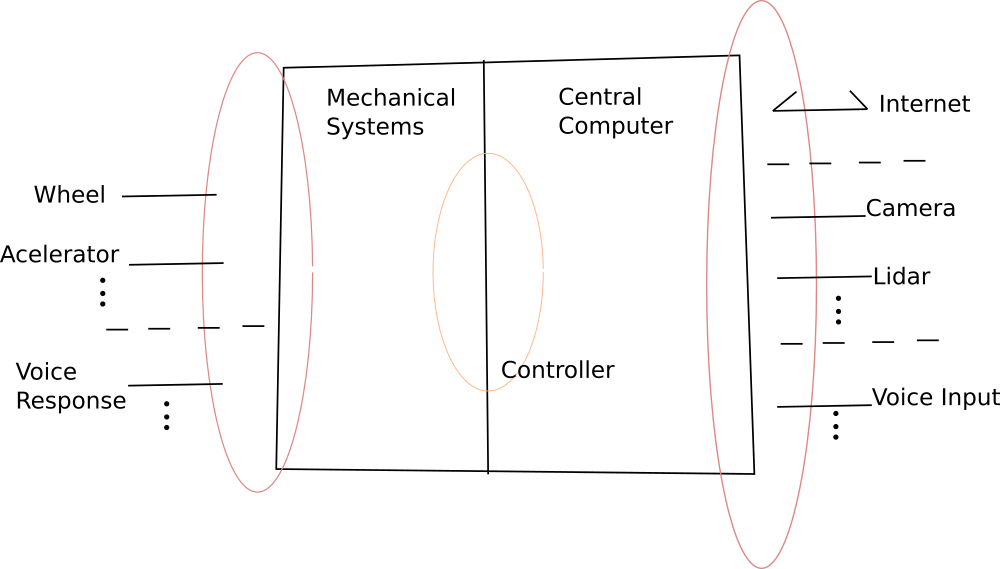
\includegraphics[width=150mm]{pics/selfDriving.png}
\caption{Self Driving Car}\label{fig:A1}
\end{figure}

We can refine this picture, as is seen in \autoref{fig:A2}. Imagine making an
initial voice command to the vehicle like ``drive to San Francisco'', which the
google voice assistant on my phone can already recognize, and plan the
\emph{initial path}. Then suppose that during the route, I get hungry and
realize I need to refuel. I can utter ``go to the grocery store after the next
exit, and then go to fuel station, but stop by the fire hydrant so I can take a
picture of that crazy sign, first.'' This is how a passenger might direct a
human driver to take a \emph{modified path}, and we take for granted that the
passenger would find it the easiest to communicate this as if the computational
agent is human. Finally, we know that neither the idealized nor the modified
path can be met without local perturbations, and that the \emph{actual path}
should be optimized to conform to the modified path relative to some metric.

The many sub-problems under this grandiose vision are themselves grandiose.
Training a neural network to accurately capture the meaning of natural language
utterances (even in a domain specific setting), the ability to synthesize a path
and a controller that meets the meaning specification, and the possibility of
following the path in an unpredictable environment - these all have large
communities working on them, and while there is certainly progress, a reliable
end-to-end system should be treated with skepticism until some kind of empirical
validation of such a system exists.

\begin{figure}
\centering
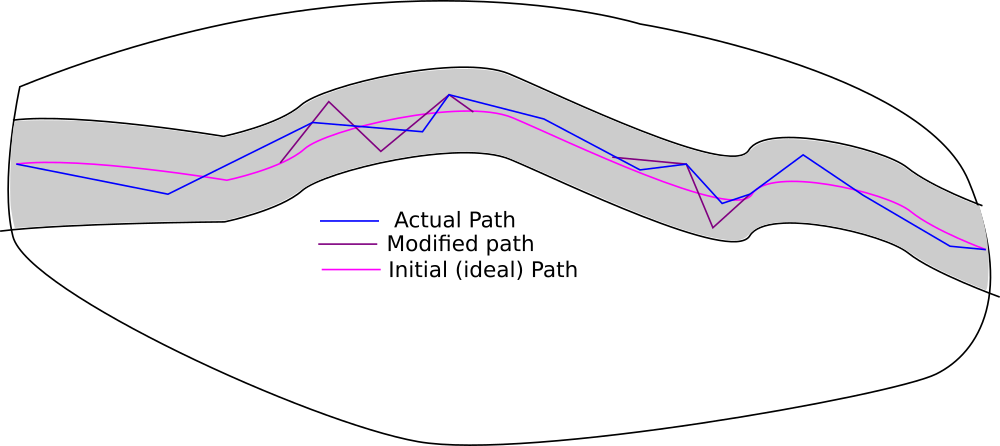
\includegraphics[width=150mm]{pics/diagramTrial1.png}
\caption{Vehicle Route}\label{fig:A2}
\end{figure}

\subsection{Overview}

Perhaps the most pervasive question in the use and application of natural
language technologies can be stated as follows : How does one optimize the
system to provide for wide coverage of the domain while ensuring that system is
robust? This question exemplifies the boundary of the verification-minded
``formalist'' and data-oriented ``empiricist'' camps in designing such
technologies.

The statistical and machine learning methods applied to Natural Language
Processing (NLP) tasks have produced impressive results over the past three decades.
They take a more pragmatic approach : compromise robustness for wide coverage,
as this means the tools will be usable and by non-experts. The belief espoused
is that the machines should ``learn'' from (and possibly like) us. Somewhat orthogonal techniques
prioritize the formal approaches of the computational linguistics communities.
These methodologies are often more concerned with theoretical justification and
explainability.

While practical tools are a goal, building practical applications often isn't
linguistically informative and therefore the empiricists' goals shouldn't
override work on building the theoretical models which enable our understanding
of the machines. Those in the formalist camp, prioritizing theoretically
informed systems, seek predictable and well-defined behavior for specific
problem domains. Yet, these systems fail to generalize without an explosion in
complexity when presented with data outside their domain.

Natural language is difficult because it is both structured with respect to
``rules'', perhaps more descriptively titled \emph{logical behaviors} which
admit lots of predictability. Yet natural language continuously breaks or
introduces exceptions to these rules, necessitating empirical and observational
understanding. This makes it exceedingly hard to penetrate with exclusively the
empirical or formalist approach. Many are led to wonder about the degree to
which large amounts of linguistic data can be augmented with theoretical
linguistic knowledge to create optimal and practical systems with respect to
both breadth and depth of coverage of language phenomena. The ultimate question
seeking compromise from both camps asks : how can we build machines which
``understand'' us (or at least our data), and which are comprehensible by us.

This problem acutely arises when trying to design a voice assistant in the
domain of commanding controllable robots, specifically, autonomous vehicles. For
the actions a vehicle takes, the motion and path decisions, must be formally
specified and controlled via some computer system subject to mathematical
formalism. Assuming the user directing the vehicle isn't aware of these
formalisms, it is incredibly difficult to design a verifiable controller capable
of dealing with the breadth of language one may encounter in the wild.

The instructions an arbitrary user gives are not subject to the same formalities
the system requires. For her commands may leave out necessary detail (``go into
the other lane'' with multiple lanes on either side), say something wrong with
respect to reality (``go into the other lane'' on a single lane road), or give a
command the driver should recognize as possible but bad (``drive directly
into the car ahead''). Additionally, the driver may need to recognize many
ways many users may say ``the same thing'', that is the same with respect to
some semantic formalism. In a dual sense, the same utterance may admit two
perfectly meaningful interpretations in two situations or contexts. The phrase
``drive to the store with the dog'' should account for whether the dog is inside
of the car. It is obviously worrisome that a nefarious actor may somehow
interfere with the controls at any stage by exploiting these manifold issues,
and indeed many more. A failure to adequately deal with these circumstances in the
vast majority of cases is not reassuring if one believes many verifiability
criteria are critical for such technologies to see adoption.

We therefore analyze our ``big-picture question'' above in the following
``sub-question'' : how can one map the manifold ways of presenting information
to an autonomous robot into a rigorous and formally verifiable kernel which the
controller can understand? Our proposed solution is to build a semantic parser
from natural language commands to linear temporal logic, whereby we can filter
the many empirical natural language commands into a ``canonical subset'' defined
by our CNL which are equivalent to (sets of) temporal logic formulas. We detail
here both the progress to these ends, as well as the challenges.

\section{Contributions}

Initially
motivated to give the system assurances against so-called
substitution-based attacks, whereby impose ``meaning equivalence'' for synonymic
expressions by imposing posterior conditions on the parse trees. Clustering via
the tree structure to provide some the equivalence to meaningfully similar
sentences was an initially enticing direction, as had been done with
Komendantskaya and Heras' work on Machine Learning for Proof General (ML4PG)
\cite{ml4pg}. However, this work had the advantage that there are multiple
large, well-maintained Coq libraries which were amenable to clustering.
Successful clustering results could give rise to proof developers seeking
suggestions in their developments.

Our use case, the design of a non-existent language, left us with the conundrum
of an impoverished data set to train over. There was no empirical data source
from which to observe ``natural ASTs'', and generating trees in an ad-hoc random basis would
not likely provide real-world applicability. What has followed should be seen as
a response to these constraints. Our intention was to find a data set suitable
to give examples of non-trivial natural language utterances, in addition to
finding a suitable semantic language with utility and applicability which is
amenable to translation from sentences parsed by our grammar. Working from both
the empirical and semantic directions seemed the most reasonable way to build a
robust least prototype of a CNL .

The primary contributions of this undertaking so far are as follows :

\begin{itemize}[noitemsep]
\item A Grammatical Framework (GF) grammar providing the definition of a CNL for
suitable directives from a passenger to a driving agent
\item A Haskell library mapping trees generated by our grammar a particularly well-behaved subset of LTL
\item An Agda implementation of LTL with a standard semantic interpretation
\item A refinement of the TOUCHDOWN dataset \cite{chen2019touchdown} suited to our needs of designing a
better grammar
\end{itemize}

 %[TODO : ref sectionions]

We suggest that while each of these components are still relatively primitive,
they define a pipeline which has potential to provide both theoretical insights
to researchers and suggest possible practical steps that can be taken to
constructing robust voice applications in industrial settings. In addition to
discussing our own contributions, we give a relevant and comprehensive literature
review that embeds our work in the context of ongoing studies about these
topics.

This work should be seen as a stepping stone, specifically we view it as :

\begin{itemize}[noitemsep]
\item A survey of existing literature about this problem
\item A preliminary work attempting to fit in pieces of a solution to the problem
\item A framework and prescription for how to fit this preliminary work carried
 out here with existing work from elsewhere in attempt to build a comprehensive solution
\end{itemize}

The feasibility of a realistic solution will doubtless rely on the future work
of many collaborators and years of research, engineering, and testing. It is
therefore naive to assume that many of the questions posed below are answerable.


\section{Preliminaries}

This research broaches many different fields, many of which were
unknown to the author prior to this work. Indeed, voice assistants may
encompass almost any natural language processing task, and autonomous vehicles are
seen as one a premier emerging robotics technology (and certainly the most talked
about in the popular zeitgeist).

Limiting the scope of work in this context can be challenging, as so many
different tools and ideas can be seen as relevant. We therefore try to very
explicitly narrow our focus to investigate how feasible it is to build a
language for an autonomous vehicle that exhibits predictable behavior and also
satisfies verification properties - this includes a determination to what extent
the properties can even be stated. As the full development of such as a system
is a grandiose vision, we hope to highlight many of the difficulties already
arising, and also those one may anticipate.

The approach taken sets out to build a semantic parser, which, despite its
primitivity, serves as a Petri dish through which many of the deeper questions
in this space may be viewed.

\subsection{Linguistic}

\subsubsection{GF, Parsers, and Personal Work}

The questions of designing an idealized and expressive formal language, with
roots in Frege \cite{frege79}, manifested more recently in the natural language
semantic tradition of Montague \cite{Montague1973}, who proposed an
interpretation of English in a typed higher order logic with a focus on
quantifiers. Aarne Ranta, a student of Martin-Löf, attempted to reformulate
Montague's work in an intuitionistic setting \cite{ranta1994type}, thereby
amenable to a natural treatment via computer programs \cite{ml79}. In
implementing a parser from natural language to a dependent type theory, Ranta
discovered that the dual sugaring (pretty printing) transformation of a tree to
a string could allow for a general mechanism of purely syntax-based translation.
This work culminated in Grammatical Framework (GF) \cite{ranta_2004}.

Grammatical Framework became a full research project, allowing for the simple
specification of a parser using a statically typed programming language whereby
the grammar rules could be seen as types. Separate concrete syntaxes cohering
with a given abstract syntax allowed for language-specific parsing, sugaring,
and translation. The GF ``standard library'', the Resource Grammar Library (RGL)
\cite{ranta2009rgl}, allows one to get off-the-shelf grammatical constructions
for more than 30 languages, with English being the most comprehensively covered. The RGL
therefore allows the grammar writer to focus on the semantic domain of the
application the grammar is being developed for. In addition to this, one can
embed a grammar as a Generalized Algebraic Datatype (GADT) in Haskell via the
Portable Grammar Format (PGF) \cite{angelov2010pgf}. One can get run-time
support for parsing and linearization directly in Haskell, in addition to
manipulating the trees by pattern matching over them as Haskell programs.

A reflection on these historical developments reveals that GF is intimately tied
to both the formal/informal distinction in addition to the syntactical and
semantical approaches present in computational linguistics. These dual characteristics
very much inform our problem as well. In the context of designing a voice
assistant for, whereby one can give commands like ``turn
right after the woman with the big dog'', we desire that the intensional belief a
user has about her utterance is consistent with the extensional behavior of the
vehicle. This can be done through an intermediary mapping to a formal semantic
representation. Ensuring that the syntactic content of a speaker's
(well-formed) utterance maps predictably to the logical form is important from
the verificationist perspective : one wants to maximize the \emph{syntactic
completeness} of the system \cite{macmillan2021}.

In a dual situation we briefly mention, one can imagine our voice assistant as
giving the user feedback, responding with clarifications (``we will turn after
the big cafe even though the other route may have less traffic''), questions
(``do you mean this or that person?''), or even possible illocutionary
directives (``we won't drive over the speed limit in a school zone''), requiring
the computer to generate an utterance after it has made some internal
determination. This internal deliberation must be a program, possibly expressed
inside or outside our semantical space. It should be capable of identifying
multiple routes in the clarification, multiple objects in a given state in the
question regarding two people, or constraints based off external circumstances
such as speed limits in school zones. In each case, the formation of a natural
language utterance requires the computer to generate natural language which must
conform to both a program's structure and behavior, but which also may be clear
and recognizable to the user.

We recognize that there are many degrees of freedom in the both the syntactic
and semantic formalisms chosen. With respect to parsing, one could choose a
categorial grammar approach \cite{5152776}, or even forego using
phrase-structure formalisms and use dependency grammars - of which there has
been recent work in using dependency formalisms in conjunction with GF
\cite{ranta2017cross}. Additionally, many of our ideas should be applicable to
robotics applications outside of the autonomous vehicle space, although
syntactic, semantic, and data-specific nuances will have to be reconsidered for
each domain.

Independently of \emph{how} the robot determines a program whose meaning it
needs to convey to a user, the property of providing a natural language
utterance which fluently conveys meaning in a natural language to some native
speaker is called \emph{semantic adequacy} \cite{macmillan2021}. Determining a
reasonable syntax and semantics for a controlled natural language should most
certainly conform to the dual standards of syntactic completeness and semantic
adequacy, if the voice assistant is to be held to any kind of regulatable
standard.


\subsubsection{Semantical Representations}

We choose LTL as our semantic form in large part due to its relative
expressivity for the kinds of verification conditions one might anticipate an
autonomous vehicle needing to carry out, in addition to its ubiquitous
appearance in the existing literature. Nonetheless, it is obvious their are many
types of logical conditions LTL doesn't immediately support, and other logics,
particularly ones which allow one to reason about space in its relation to time,
would be an ideal direction to look. This line of research is probably more
suited to people developing systems at later stages of development, where
empirical observations may be collected in the wild. The nuances of where an
autonomous navigator responding to a human agent can go wrong, and the most
amenable set of verification conditions to prevent this, will ultimately have to
be gained through trial and error.

\paragraph{Notions of Semantics}

We also note that the notion ``semantics'', having many connotations and interpretations in
different fields, is subject to many interpretations. Here are some examples :

\begin{itemize}

\item In linguistics, semantics may be interpreted as intended meaning.
Different theoretical notions of meaning may include a logical meaning, as in
the case of Montague semantics, or a meaning as it arises in the use and context
of culture, as is the case of cognitive semantics.
\item In programming languages, the semantics of a syntactic entity most
commonly means the mathematical behavior (denotational semantics) or behavior
during execution (operational semantics).
\item In statistical notions of semantics, one often seeks the ability of one to
capture meaning via language use, most common in contemporary contexts, its
practical uses. Frequently Word2Vec \cite{word2vec} is referenced in this context,
although the advent of transformers in recent years has largely usurped this.
\end{itemize}

The problem presented in our work, of speaking to a machine, presents challenges
in that it requires notions of semantics from disparate disciplines, which
themselves have little overlap (at least as treated in the existing literature).
This is because we are attempting to witness an utterance as a natural, native
linguistic phenomena with an indented speaker meaning, a program whose syntax is
defined via the CNL, and a statistical observation defined over some probability
distribution of ``sayable things''. More concretely we ask :

\begin{itemize}
\item How is the speakers meaning interpreted as if intended to be understood by
 other native speakers?
\item How does the speakers meaning manifest as a formal program a computer can
 evaluate?
\item How can we identify a speakers meaning in a possibly infinite space of
 utterances and contexts in which those utterances arise, neither of which can
 be formally defined \emph{a priori}?
\end{itemize}

Although the inter-relatedness of various semantic theories is a much bigger
project than we can give space to here, it should be granted that problem we
address forces one, both implicitly and explicitly, to try to grapple with them.
We chose \emph{the syntax of LTL} as the \emph{semantics of our CNL} which is
defined by filtering a ``naturally observed'' corpus to a primitive grammar. We
propose to fit unseen utterances by fine-tuning a transformer-based language
model to the corpus and grammar. We can then seek specific formalisms in which
to analyze our problem domain :

\begin{itemize}
\item The meaning for a passenger-speaker can be analyzed in a variety of ways :
 \begin{itemize}
   \item The meaning of an utterance is a logical formula following Montague's
   lead, substituting temporal operators for generalized quantifiers.
   \item That the passenger's utterance should be determined as a speech act
     which carries illocutionary force and intention. The computer's
     response can be seen as conforming to or negotiating with the desires of
     the user, subject to the computers internal constraints and possible
     contextual information about which user may be unaware. Applying speech
     act theory in the context of human computer interaction has a long history
     \cite{winograd}.
 \end{itemize}
% from wikipedia
% The key insight provided by Winograd and Flores is that the state-transition diagram representing the social (Illocutionary) negotiation of the two parties involved is generally much, much simpler than any model representing the world in which those parties are making claims; in short, the system tracking the status of the conversation for action need not be concerned with modeling all of the realities of the external world
\item The meaning of the syntactic formula, can be interpreted in many possible ways
 \begin{itemize}
   \item A type specification. In a case where
     temporal logic formulas are interpreted as types, Functional Reactive
     Programming (FRP), provides a functional programming context with which to
     interpret temporal formulas
     \cite{hudak}.
   \item A (possibly verifiable) motion planner  \cite{verifiedMotion} \cite{7759412} \cite{kuo2020deep}
   \item A dialogue state, in the envisioned Question Answer (QA) context, whereby
     the computer must provide feedback to the user based of contextual information
 \end{itemize}
\item The meaning from the mostly unseen utterances is given a canonical form,
 and the canonicalization process is a transformation via the vector-space and
 distributional notions of meaning implicit in an attention-based neural network
\end{itemize}

We don't intend to exhaust the list of possibilities here, neither in our
description of the many meanings of ``semantics'', nor in how our taxonomy of
semantics can be understood in the context of our solution to the problem of
giving navigation commands to a autonomous driver. We intend to clarify some of
the many subtleties and terminological confusions arising from many
communities of researchers. We suggest that working towards a unified view of
what kinds of semantic notions we want to deal in this particular domain may
inform better solutions to the problem at hand.

\paragraph{Semantic Parsing}

The problem of semantic parsing consists of mapping natural language utterances
not just to syntactic trees, but to semantic ones. A sub-field of Natural
Language Understanding (NLU), building automated systems for mapping syntax to
semantic forms can be traced back to Winograd's SHRDLU
\cite{winograd1971procedures}. Although seen as a success at the time, SHRDLU
was also incredibly brittle, and apparently led Winograd to step away from NLU,
believing the problem too difficult.

The largest strain of contemporary interest in semantic parsers emerged during
the resurgence applying deep neural networks to a variety of problems in NLP.
An important observation, to view ``semantic parsing as paraphrasing''
\cite{berant-liang-2014-semantic}, has greatly influenced the contemporary
statistical approaches to semantic parsing. Much of this work has still used
grammars as a central component in their  pipeline, often to generate sentences
randomly for the construction of a corpus to train with.

Towards the extreme of the data-centered perspective, it has been advocated to
get rid of the parser in semantic parsers altogether. In \cite{dontParse}, the
authors naively takes for granted large public data-sets with syntactic and
semantic forms, neither of which exist for autonomous vehicle syntax and
temporal logic semantic formalism. Our approach takes for granted that the
parser is one of the most controllable and easily understood components of a NL
pipeline.

\paragraph{Semantic Parsing for Temporal Logics}

\begin{quote}
given an input English utterance, preprocess it to extract syntactical information, which may
include part of speech tagging, dependency parsing, semantic role labelling, and so on. Then,
enrich the input with these pieces of information. Finally, run an attribute grammar-based
parser, or rely on some hand-made rules, to derive a translation into a target logical format.
\cite{brunello_et_al}
\end{quote}

Brunello et al. give a thorough literature review of the many ways of
translating natural language to LTL, indicating the interest and need of
suitable semantic parsers in this domain. We give a refined perspective on the
problems below, deferring a formal treatment of LTL to the appendix [TODO :
reference].

An interesting result published more recently attempts to translate between
English and Signal Temporal Logic (STL) \cite{he2021english}, which has the
advantage of not just treating Boolean, but real-valued signals. From this
perceptive, STL vs LTL can be understood as a quantitative versus qualitative
way of analyzing events. The fact that STL gives the specifications a higher
expressiveness in terms of how the order of events takes place, but also comes
with a higher computational cost [ref needed], but more importantly, a
potentially unnecessary complication for the system designer, The more
granularity view of time may be unnecessary in many cases - our data set doesn't
cover time at all (a defect, [reference below]), but even in a more naturally
derived corpus, might only crop up as an ``edge case'' relative to other more
important or likely phenomena that engineers may wish to capture.


\subsection{Robot Motion Planning and Verification}

The challenge of designing a system which generates robot control strategies
from human language has to balance the expressiveness of task specification,
complexity of environment, and provable correctness \cite{4141034}. In this
context, we assume that expressivity of the language itself should reflect the
complexity of the environments, thereby being adequately descriptive. The
criteria of correctness : that the language itself is well-represented in the
LTL semantics - the system being is syntactically complete - is the focus of
these investigations. Our work additionally, is the only work we know of which
actually seeks autonomous vehicles as the central motivation, rather than more
general robotics applications.


\subsubsection{Temporal Logic for Robot Verification}


We need a comprehensive view of the robot control problem as it pertains to
temporal logics. Our considerations should include :

\begin{itemize}
\item The kinds of logical behavior one may wish to capture
\item The sorts of missions we want our autonomous agent to accomplish
\item The types of atomic grounded conditions one may want to include
\item How do we model both the vehicle and the environment
\item How do these logical behaviors interface with other components of the
 larger system
\end{itemize}

\paragraph{Temporal Logics}



Modal logics, specifically those dealing with stateful staging of events like
LTL \cite{ltl95}, Computation Tree Logic (CTL) \cite{yooCTL}, Signal Temporal
Logic (STL) \cite{stlAut} , have been used extensively in the specification and
verification of properties of robotics systems, including autonomous vehicles .
As LTL is often seen as one of the ``primitive'' temporal logic, we chose it as
a our semantic space despite its limitations (the lack of numerical precision,
predicates for spatial relations, etc). We appreciate that future work will need
to expand the scope of which logic (or possibly \emph{logics}) the machine may
use to verify behavior, in addition to the mathematical models most amenable to
verification of a logical formula.

% ugg
% Additionally, LTL  formulas can be transformed into automata which can then be used as reward
% functions for reinforcement learners, as in \cite{ltlRein}.
As regards the logical behavior, there are an array of logics available.

\begin{itemize}
\item Linear Temporal Logic (LTL)
\begin{itemize}
\item
\item
\end{itemize}
\item Metric Temporal Logic (MTL)
 go to the store within 5 minutes
 modal operators can express timing constraints
\item Signal Temporal Logic (STL)
 the paths and models are now signals
 can be appended with a metric semantics, to show how well a formula satisfies
\item Computation Tree Logic (CTL)
 follow the car in front of us
\item CTL*
\item Probabilistic Computation Tree Logic (PCTL)
 %go to the store if its unlikely we'll hit bad traffic
\end{itemize}


% Co-safe LTL (non-reactive): (¬Deliver ) U(Deliver ∧(Office B ∨Office C )) expresses “deliver
% a package to one of offices B or C but not anywhere else” .
% GR(1) fragment (reactive):  
%  (SensePackage → (Deliver ∧ (Office B ∨ OfficeC ))) ∧
%  
%  (¬SensePackage → Mailroom) expresses “If you sense a package then deliver it to
% Office B or Office C, otherwise go to the mail room” (only part of the formula is shown).
% PCTL: P>0.95 ( 
%  (Deliver ∧ (Office B ∨ Office C ))) expresses “The robot should deliver the
% package to Office B or C with probability greater than 0.95”.
% STL: 
%  [0,5](Deliver ∧ (Office B ∨ Office C )) expresses “Deliver the package to Office B or
% Office C within 5 time units”


% LTL satisfiability is decidable in polynomial space.
% LTL validity is decidable in polynomial space.
% LTL model checking is decidable in polynomial space

% CTL model checking is decidable in polynomial time.
% CTL satisfiability is decidable in exponential time.

% CTL∗ model checking is decidable in polynomial space.
% CTL∗ satisfiability is decidable in doubly exponential time.

%  Model checking and satisfiability for MTL in the point-
% wise semantics over finite words are decidable but non-primitive recursive. Over
% infinite words, both problems are undecidable.

%  Model checking and satisfiability for MTL in the continuous
% semantics (over both finite and infinite signals) are undecidable.

\paragraph{Missions Types}

In the literature, there are two main properties of concern
when specifying robot behaviors to be checked by models : \emph{safety} and \emph{liveness}.
These are intimately related to the temporal modalities. Safety
properties say ``nothing bad ever happens'', that is, a specification is
satisfied globally by some model. Liveness conditions, on the other hand, mean
that ``something good eventually happens''. An important theoretical result is
that safety and liveness are expressively adequate : every property of interest can be
decomposed into safety and liveness components \cite{Piterman2018}.

This distinction is particularly relevant for our analysis, because we suggest
that for the most part, directions given by a human (at least in our fragmented
treatment) should be interpreted as liveness conditions. The
expression of the desire to reach of a sequence of destinations, says that
eventually we arrive at each such destination.

On the other hand, when we account for behaviors of the vehicle that are
generally not intended to be instructed by the driver, these should be
interpreted as safety properties. Obeying all traffic laws can be treated as a
global condition that the neither passenger, nor an adversarial attacker should
be able to override. Additionally, ``comfort properties'', like assuring the
vehicle never accelerates too quickly or takes turns too quickly could also be
encoded in this way. While there may be other mechanisms of enforcing or
verifying that a vehicle meets these standards, we envision that the route
planner (and the verifier) should treat the linguistic utterance as saying that
do something good while simultaneously always never behaving badly.

We now discuss the missions that a user would want to instruct a vehicle to
carry out, in the context of satisfying a stack of safety property
preconditions. In \cite{specPat}, the authors empirically analyze an array of
literature about robots and the types of missions they are typically employed
for, filter out a subset of generalized LTL formulas which appear frequently,
and design a tool PsA1M capable of building template missions over these formulas.
We pay particular attention to what they call ``core movement patterns'', which
include coverage (mainly what we're concerned with) and surveillance (which
could be relevant, if, for instance, one wanted to design a autonomous-taxi that
surveils a region of interest for passengers).

The coverage properties consist of visiting a set of locations, where various
extra conditions like sequencing, ordering, and strictly ordering governs how.
Specifically, given a finite (or incomplete) set of locations or events $\{l_i\}$
where $i \in \{1..n\}$ we can say a baseline coverage is of the form
$\underset{i}{\bigwedge}\; F\; l_i$, which due to the commutativity of conjunction,
doesn't distinguish between the order in which the locations are visited. To
ensure that for every location $l_i$ eventually follows its predecessor $l_{i-1}$, we
nest the locations in future temporal operators, essentially building a linked
list $F\; (l_1 \wedge F\; (l_{2} \wedge ... F\; l_{n}))$ with an extra $F$
operator appended at every node. To induce the ordering, we can conjoin a predicate
which restricts how the locations are sequenced by imposing the condition that location
$l_{i}$ must be visited prior to its successor $l_{i+1}$, namely
$\underset{i}{\bigwedge}\; (\neg l_{i+1})\; U\; l_i$.
If one wants to also ensure that the locations aren't redundantly visited, we
can add the strictness condition. A bit confusing,

$\underset{i}{\bigwedge}\; (\neg l_{i})\; U\; (l_i \wedge X\; (\neg l_i\; U\;
l_{i+1}))$, this property ensures that one cannot revisit location $l_i$ until
after it has been initially visited and, in the next time increment, it hasn't
been visited until its successor location $l_{i+1}$ has. To see how these syntax
trees are encoded in Agda, please see the appendix [TODO:REF].

As concerns directing autonomous vehicles, one anticipates that the user
generally would want a sequential visit, with the order condition presumably but
not necessarily intended in most situations. The strict order condition seems
like it would need to be induced by the system almost automatically for
efficiency reasons. We therefore chose to target the vanilla sequential visit
with our Haskell program, although it merits a close investigation in which
circumstances other logical predicates should be inferred, both based of
specific language of the passenger and other contextual constraints.

Other movement patterns may reference past tense temporal operators, which may
indeed prove very useful to verify that a users needs have been met, or the
cases in which the route taken didn't conform to a command. We envision that
developing a complete calculus of specification patterns in the specific domain
of autonomous vehicles should very much inform how the CNL should be designed.

\paragraph{Environment and Grounding}

The historical development of logic in mathematics ultimately served to
partition the mathematical expressions so that one could abstract the high level
reasoning, the proposition and a proof structure, from the purely mathematical
constructions. The interpretation of types in programming as logical
propositions emanating from constructivist circles questioned this partitioning,
allowing one to construct computer programs with mixed and indistinguishable
``logical'' and ``mathematical''. In the case of temporal logics for
cyberphysical systems, however, the atomic propositions like ``is-green-light'',
``truck-ahead'', or ``grocery-store'' have no simple encoding in programming
languages. This is because they aren't mathematical precise concepts, being
empirically fastened to the environment in which the computer program operates.
This is an incredibly important realization : how we witness the world is
captured by some possibly faithful but incomplete mathematical abstraction.

For the atomic propositions in a temporal sentence to have meaning, we must
ground them to the physical world. This grounding involves both the sensors
collecting data from the physical environment, as well as the mathematical
approximations we make of the environment. In \cite{synthGazit}, the authors
review the many ways one can take propositions in various temporal logics and
synthesize `` correct-by-construction robot controllers'', in the case there is no
contradictory evidence about a specification's feasibility. Although this
synthesis process exceeds the boundaries of the work, it is important to discuss
because how one models the external environment and the events in it, should
cohere to the internal environment - the natural language instructions.
When building a system, reasoning about it from both directions is paramount.

Explicitly, how one chooses to approximate the external environment, and what a
vehicle can and should \emph{do} in it, should inform the constraints what
one can say in the internal environment. In the case of a QA system where the
car needs to inform the passenger of why the vehicle can't obey such
instructions, or ask for clarification, the Natural Language Generation (NLG)
phase will need to perform some kind of ``reverse synthesis'', and this process
may well be much more difficult than the synthesis process to begin with.

The paper details three main ways of approximating the continuous external
environment, modeled as a dynamical system specified by a first order
differential equation, by a state transition system. These abstractions are from
the dynamical system to a symbolic model represented by a transition system are
partitions, motion primitives, and motion planners with trajectories. The partitioning generates a
discrete transition system from a continuous state space, where actions
represent movements between areas, and is contingent upon the dynamics of the
differential equation. The motion primitives approach defines the primitives as
maps between a different kind partition of the state space, and it is noted that
they definitionally satisfy invariance and liveness properties, ideal for our application.
To generate paths without regard to the dynamics of the system, motion planners
deal with a geometric partition and builds robot trajectories based off where
the robot is at a given time.

Once the abstraction from the external environment to a transition system has
been realized, the translation of a logical formula into a Buchi Automata (or
some other automata) can decided true or false relative to the Kripke model
which has been generated. Unfortunately, the generation of an automata is doubly
exponential in the size of the LTL sentence.

Using a tame fragment of LTL, Generalized Reactivity (1) (GR(1)), one may use
game-theoretic approaches to that reduce the complexity of controller synthesis
to polynomial in the size of the external environment's transition system
\cite{BLOEM2012911}. The GR(1) fragment partitions the atomic propositions into
two sets based of the environment and the state. Those formulas $\phi_e$ which
represent environmental sensor data, and those propositions tied to the robot
state, $\phi_s$, grounded to actions and physical positions. The fragment deals
with sentences of the form $\phi_e \implies \phi_s$, where both sets of formulas
can be seen as a conjunctions of initial conditions, safety assumptions, and
liveness conditions. In our example, this would mean that the command like
``turn right at the fire hydrant'' could enable (constructive) validation of the
condition by ensuring that a camera takes a photo which shows a fire hydrant
within some distance, then the car must be at a GPS certain coordinate on some
map which has a fire hydrant, and that this should precede a state where the car
sense a turn coupled with the steering wheel turning.

Unfortunately, the liveness conditions only allow for formulas of the form
$\underset{i}{\bigwedge}\;G\; F\; \phi_i$ with $\phi_i$ restricted to using
Boolean connectives. Nonetheless, by isolating environmental sensor data from
the position certain and action primitives, and additionally separating out the liveness
and safety properties, we see a clear methodology that can greatly simplify our
specific problem. It is not known to the author if there has been work
investigating synthesis coverage properties the fragment of LTL for the coverage
properties, but it is well worth investigating, because despite the nesting of
the $F$ operators, we can certainly anticipate a reduction in the complexity of
these types of formulas.


% for a distinction between Planning Domain Definition Language (PDDL)
% The differences between synthesis approaches and those pursued in the planning community
% span the way the problem is formulated, the complexity of the algorithms, the expressive-
% ness of the specifications and system models, and the type of feedback that is possible when
% the synthesis/planning problem can and cannot be solved.


\paragraph{Environment and Vehicluar Modeling}

\paragraph{External and Other Constraints}

Linear logic, resource sharing, etc

The review \cite{synthGazit} forgoes dealing with multi-agent systems,

\section{Our Pipeline}

As mentioned in the [TODO : Ref contributions], this work makes a proposal for
how to create a general semantic parser from arbitrary voice commands to the
coverage and sequencing subset of LTL, maximizing both coverage and robustness
of the system. We outline the work done with respect to the following pieces, of
our system, and conclude with the proposal which envisions a synthesis of all
these pieces.

\begin{itemize}[noitemsep]
\item A refinement of the TOUCHDOWN dataset \cite{chen2019touchdown}
\item A refined version of the touchdown dataset
\item A GF Grammar
\item A PGF Haskell embedding of the Grammar
\item An Agda implementation of LTL [TODO: see appendix]
\end{itemize}

\subsection{Touchdown Data Set}

The most comprehensive known data source relevant to this problem is the
TOUCHDOWN data set \cite{chen2019touchdown}. The authors' used Amazon Mechanical
Turk workers and an ``interactive visual navigation environment based on Google
Street View'' based off images collected in New York City to generate English
Language instructions to describe a route based off the visible environment to
find a ``touchdown object''. Once the object is visible, the task is complete.

An intention of the work is a seemingly natural dataset which accounts for
``resolving the spatial descriptions'', but we focus only extracting the
navigation instruction part of the task, knowing that the image classifier and
the grounding mechanism is outside the scope of our work. Although the data
comes equipped as JSON files with the text itself, a coordinate mapping
instructions compatible with streetview, and other metadata, we just focus on
the natural language text. The text samples consist sequence of constructions with
visible cues, terminating with a description of where to find the ``touchdown''.
A typical of the text is :

\begin{quote}
Orient yourself so you are following the flow of traffic, Continue straight
until you reach the intersection and take a left, You should see a red bus lane
to your right and a bus stop, Continue straight until you are just past the bus
stop, look to your right and you will see a tree with yellow foliage, click the base of the tree to find touchdown.
\end{quote}

When filtering the dataset, we can choose to uniformly replace the last sentence
reference the ``touchdown'' with the word finish. We first indicate some of the
advantages of this data set with regards to our application.

\begin{itemize}
\item The size is reasonably large with approximately 10000 multi-command instruction sequences
\item The descriptions are full of linguistic nuance and diversity
\item The data is collected from multiple users, and is methodically produced
\item The non-linguistic data may be of interest to those investigating
how to grounding the utterances to the Street View panoramas
\end{itemize}

We imagine to a first approximation, these sequences are a great starting point
when trying to build a robust system with respect to the linguistic environment.
Nonetheless, there are many potential drawbacks, both with the data collection
process itself, and the application we have in mind. These include :

\begin{itemize}
\item Finding the touchdown only coarsely approximates general navigating in a city.
\item The data is limited to New York City, which is mostly a hectic urban environments,
 and takes streetview images from only the day.
\item The workers don't necessarily know New York, so everything the reference is in their immediate
 visual environment.
\item This is a ``short-term'' task, it requires no long-distance navigation
 and reasoning.
\item Working with panoramas is not necessarily a great simulation to a real
 environment. This manifests in, for example, frequent use of the word choice
 of ``walk'' instead of ``drive''.
\item ``The workers are not permitted to write instructions that refer to text in the
images, including street names, store names, or numbers''  \cite{chen2019touchdown}
\item No explicit temporal reasoning with regards to actual and relative times,
 i.e. ``noon'' and ``in 5 minutes'', respectively
\item The limitations of using panoramic image data
\item The fact that Amazon Turk workers are exploited. This may influence how they
 do the work (they try to meet the standard that makes them the most amount of
 money), and also not be a representative sample of the population.
\end{itemize}

A truly ideal data set would resolve these issues and meet the following
criteria :

\begin{itemize}
\item The instructions would consist of long and short distance driving tasks,
 preferably interspersed.
\item The data set would include different urban and rural areas, different
 languages, non-paved environments, different weather and lighting conditions, and possibly multiple speakers in the car
\item The passengers would be more diverse and have vary degrees of contextual
 information like street place, public names like ``the opera'' and
 private names like ``mom's house'' (whereby a named entity recognition would
 be very important component)
\item Collecting the data ``in the wild'', envisioning a cab with a human
 drivers equipped with sensors and microphones
\end{itemize}

That the data collection task in an objective way is inherently tied to the way
we collect the data, approximating the world and environment. This limitation is
over one's whole experimental apparatus and assumptions in designing the data set.

\subsubsection{Filtering the data set}

Once the natural language commands were extracted from the touchdown JSON file as a preprocessing stage,
we sought to curate the data so that it is more compatible with our GF grammar. We ran the Stanford part-of-speech tagger
\cite{toutanova-etal-2003-feature} over the command sequences, modified with a
``Finish.'' sentence substituted for the touchdown phrase to indicate command
termination.

We to process the data so that it enables both generation of a GF grammar which
parses at least a minimal skeleton of the linguistic diversity found in the
corpus. As GF grammar is not capable of directly interfacing with out-of-the-box
part-of-speech-taggers at the \emph{concrete syntax level} when using the RGL
because of a mismatch of grammatical categories, it is at the \emph{abstract
syntax level}. While this is a potentially important line of research - to
interface GF deal with tagged data-sets - the n-gram language model over
the corpus  lexicon is very capable of informing the GF grammar.

The processing of the data in Haskell was simple : we simply ordered the n-grams
of the whole words of the corpus by frequency and (n-gram) POS label, and this
was easily done with basic functional programming techniques operating over
nested lists and tuples, although in the future it would certainly be better to use a lens
interface. For instance, one can quickly filter the most common
POS-ngrams to discover that ``go'', ``be'', and ``turn'' are the most frequent
verbs, and that the most frequent POS-trigrams of the form \emph{(preposition,
cardinal number, singular or mass noun)}, are ``through one intersection'', ``for
one block'', and ``between two silver''.

One interesting facet of this data set is the high count of certain ``big n''
n-grams : the 9-gram ``so you are moving with the flow of traffic'' occurs 311
times in the corpus. This regularity indicates how domain specific the corpus
is, and also indicates the most important phrases to include in the grammar.

\subsection{GF Grammar}

\subsubsection{Brief Intro To Gf}

A grammar specification in GF is an abstract syntax, where one specifies trees,
and a concrete syntax, where one says how the trees compositionally evaluate to
strings. Multiple concrete syntaxes may be attached to a given abstract syntax,
and these different concrete syntaxes represent different languages. An AST may
then be linearized to a string for each concrete syntax. Conversely, given a
string admitted by the language being defined, GF's parser will generate all the
ASTs which linearize to that tree. The composition of parsing and linearization
amounts to machine translation.

When defining a GF pipeline, one has to merely to construct an abstract syntax
file and a concrete syntax file such that they are coherent. In the abstract,
one specifies the \emph{semantics} of the domain one wants to translate over,
which is ironic, because we normally associate abstract syntax with \emph{just
syntax}. However, because GF was intended for implementing the natural language
phenomena, the types of semantic categories (or sorts) can grow much bigger than
is desirable in a programming language, where minimalism is generally favored.

The two functions displayed in \autoref{fig:N2}, $Parse : \{Strings\}
\rightarrow \{\{ASTs\}\}$ and $Linearize : \{ASTs\} \rightarrow \{Strings\}$, obey
the important property that :

$$\forall s \in \{Strings\}. \forall x \in (Parse(s)). Linearize(x) \equiv s$$

Both the $\{Strings\}$ and $\{\{ASTs\}\}$ are really parameterized by a grammar
$G$.

\begin{figure}
\centering
\begin{tikzcd}
Strings \ar[r,"Lexical\ Analysis"] \ar[rr,bend right,"GF\ Parser"'] &[10em] Lexemes
\ar[r,"Parsing"] &[10em] ASTs \ar[ll,bend right, "GF\ Linearization"]
\end{tikzcd}
\caption{GF in a nutshell} \label{fig:N2}
\end{figure}

\subsubsection{Our Drive Grammar}

We present a simple proof-of-concept grammar, to illustrate these ideas above.

The abstract syntax consists of two declarations, where one defines
\emph{categories} with ``cat'' and simply typed function signatures over those
categories, denoted by the ``fun'' keyword. GF has support for dependent types
as well, although they make general parsing undecidable and are relatively
unmaintained.

The first thing we want to recognize before delving into the details of our
Grammar is that the directive-style commands, being informed by the intended
downstream LTL semantics sequencing, namely, the car visiting a series of
locations $l_i$ in some not necessarily strict order, given the form $F\; (l_1
\wedge F\; (l_{2} \wedge ... F\; l_{n}))$.

As the core driving controls of the vehicle are limited to an accelerator,
break, and steering wheel, we can look at verbs from the corpus, to the
recognize that only present tense, base-form verbs ``VB'' inform these. Other
POS verb classifications - past -tense ``VBD'', gerund ``VBG'', past participle
``VBN'', singular present, 3rd person or not, ``VBP'' and ``VBZ'' respectively -
either seem to describe a scene or object in the peripheral environment or the viewers
relationship to some such happening. We show the counts of the top verbs
processed by our Haskell script.


\begin{verbatim}
  ([(["Go"],5527),(["be"],5300),(["turn"],4154),(["Turn"],4154)],["VB"])
  ([(["left"],228),(["came"],59),(["made"],47),(["started"],44)],["VBD"])
  ([(["going"],1684),(["facing"],939),(["moving"],849),(["passing"],617)],["VBG"])
  ([(["left"],1733),(["parked"],616),(["painted"],307),(["fenced"],263)],["VBN"])
  ([(["are"],3554),(["'re"],1185),(["reach"],1100),(["get"],770)],["VBP"])
  ([(["is"],4919),(["has"],795),(["'s"],471),(["ends"],93)],["VBZ"])
\end{verbatim}

The exception is the base-form ``be'', which
typically denotes things are relative to you. So if one says ``go to the store
and there should be a mailbox on your right...'', the logical condition could be
indicated as $F\; (theStore \wedge aMailboxOnRight \wedge ...)$, whereby being
at the store is next to a mailbox are simultaneous properties to verify.

One recognizes that the relationships of the driver to the scenarios described is to
be understood with respect to the camera and the sensors, with the vehicles spatial/temporal relationship to
them dealt with by the grounding mechanism. We therefore organize our commands
based off the most frequent verbs : go, turn, stop, ...)

We now indicate the main ``semantic'' content of our parser, whereby our
primitive ontological categories are listed alongside example strings which
are grammatical examples parsible and linearizable with respect to the
linearization.

\begin{verbatim}
cat
 Command      ; -- don't go to the store
 Polarity     ; -- don't
 PosCommand   ; -- go to the store
 Place        ; -- the store
 Time         ; -- in 5 minutes
 Action       ; -- drive
 Way          ; -- to
 How          ; -- quickly
 Where        ; -- left
 AdvPh        ; -- to the store
 UndetObj     ; -- store
 Determ       ; -- the
 Object       ; -- the store
 Number       ; -- a
 Conjunct     ; -- and
 Condition    ; -- there is a museum
 Descript     ; -- big
\end{verbatim}

These categories form the core calculus for building imperative commands. To
construct them we must specify the functions, of which we only sample a few. We
first notice that categories like ``Descript'', ``Conjunct'', ``Where'' are all
limited to single words, whereas the phrases must be syntactically composed - and
this composition is given by plugging in sub-expressions in the AST, typable via
simple functions over the categories. We list a subset of the grammar ordered by
relative proximity to the root of the tree.

\begin{verbatim}
 DoTil     : Action   -> Time         -> PosCommand ;
 SimpleCom : Action   -> PosCommand ;
 Finish    : PosCommand ;

 ModAction : Action -> AdvPh -> Action ;

 MkAdvPh     : Way   -> Object -> AdvPh ;
 HowPhrase   : How   -> AdvPh ;
 WherePhrase : Where -> AdvPh ;

 WhichObject : Determ -> UndetObj -> Object ;
 ObjectPlace : Place  -> Object ;

 ModObj : Descript -> UndetObj -> UndetObj ;

 InNMin : Determ -> Way -> Time ;

 MkNum  : Int -> Determ ;

 Quickly : How      ;
 Left    : Where    ;
 Around  : Where    ;
 To      : Way      ;
 After   : Way      ;
 Store   : UndetObj ;
 Traffic : UndetObj ;
 Car     : UndetObj ;
 Person  : UndetObj ;
 London  : Place    ;
 Drive   : Action   ;
 Turn    : Action   ;
 Big     : Descript ;
 A       : Determ   ;
\end{verbatim}

We since the sequence consists of multiple locations, each of which may satisfy multiple
conditions, we need to \emph{listify} certain categories. We can include
judgments like \gray{cat [PosCommand]{n}}.
GF natively supports list categories, the judgment \gray{cat [C] {n}} can be
desugared to

\begin{verbatim}
 cat ListC ;
 fun BaseC : C -> ... -> C -> ListC ; -- n C ’s
 fun ConsC : C -> ListC -> ListC
\end{verbatim}

This introduces new categories and functions : for instance, one may induce
lists of positive commands by introducing a list of positive commands which can
be which, can then be coerced back into a ``single command'' so that the string
``go to the store and turn left'' can be parsed by adding including the
following judgments, noting the last two are automatically generated at compile-time :

\begin{verbatim}
  cat [PosCommand]{2};
  fun
    CompoundCommand : Conjunct   -> [PosCommand] -> PosCommand   ;
    BasePosCommand  : PosCommand -> PosCommand   -> [PosCommand] ;
    ConsPosCommand  : PosCommand -> [PosCommand] -> [PosCommand] ;
\end{verbatim}

One can include an explicit \gray{cat Commands;} to enable punctuation denoting
full sentence structure, which should also be listified. We reveal a parse tree
example from the GF REPL.

\begin{verbatim}
p " go to the store , turn left  and stop . Finish ." | tt
* ConsCommands
    * OneCommand
        * CompoundCommand
            * And
              ConsPosCommand
                * SimpleCom
                    * ModAction
                        * Go
                          MkAdvPh
                            * To
                              WhichObject
                                * The
                                  Store
                  BasePosCommand
                    * SimpleCom
                        * ModAction
                            * Turn
                              WherePhrase
                                * Left
                      SimpleCom
                        * Stop
      BaseCommands
        * OneCommand
            * Finish
\end{verbatim}

One should notice that the tree is not subject to arbitrary branching. In fact,
this is evident that if one starts walking around the exterior of the tree, that
the leaves consist of expressions which linearize to ``the store'', ``left'',
``stop'' and ``Finish.''. Indeed, these are exactly and only the sequence of
places and conditions one imagines the vehicle going to and satisfying during
a trip. Our grammar is designed such that the abstract syntax reflects a linear
ordering of the atomic conditions, and therefore allows for a straightforward
denotation as a canonical template formula $F\; (l_1 \wedge F\; (l_{2} \wedge ... F\; l_{n}))$.

\paragraph{Linearization}

While the abstract syntax is a sort of ``neutral syntax'', attempting to specify
and capture the structure, meaning, and ontology of a given domain, the concrete
syntax realizes this via different models, manifest as languages : sets of
strings whose concrete form must cohere to the abstract structure.

The concrete syntax introduces two complimentary declarations. The first is
linearization types ``lincat'', which essentially consist of strings, finite
number types, and products (manifest as records). From this calculus one can
encode coproducts as well, which one has access to as well. The function bodies
are given via the ``lin'' declaration. There are operator and parameter
declarations which serve as auxiliary means of prettifying one's code.

We utilize the RGL, with the API guiding most of the implementation details.
This allows us to focus on any particular domain specific or syntactic
phenomena, delegating morphological details like tense, aspect, and number to the RGL
authors. This does raise an interesting point : the RGL, enabling more
expressive grammars ``out the box'' can actually hide morphological detail which
may be semantically relevant for a given situation. Therefore, one would need to
account for number in designing the above abstract syntax if one wants the
references ``person'' versus ``people'' to be distinguished as atomic elements
which may be grounded differently.

Importing from the RGL, we show the linearization categories coherent with those above.

\begin{verbatim}
lincat
  Commands     = Text        ;
  Polarity     = Pol         ;
  Command      = Utt         ;
  [PosCommand] = [Imp]       ;
  PosCommand   = Imp         ;
  Conjunct     = Conj        ;
  Action       = VP          ;
  Way          = Prep        ;
  AdvPh        = Adv         ;
  How          = Adv         ;
  Where        = Adv         ;
  Time         = Adv         ;
  Place        = NP          ;
  Object       = NP          ;
  Determ       = Det         ;
  Number       = Det         ;
  UndetObj     = CN          ;
  Descript     = SyntaxEng.A ;
  Condition    = Cl          ;
\end{verbatim}

If one goes into the RGL source, we can see a sample of the linearization
categories. For instance, in English an common noun \gray{CN} has an inherent
gender given by a field \gray{g : Gender}, which is just a ternary parameter
type with three constructors but may manifest differently
depending on if its singular or plural, and whether the case argument indicates
a possessive relation. We quote the relevant parts of the RGL :

\begin{verbatim}
  lincat
    CN = {s : Number => Case => Str ; g : Gender} ;
  param
    Gender = Neutr | Masc | Fem ;
    Number = Sg | Pl ;
    Case = Nom | Gen ;
\end{verbatim}

By abstracting away these details within our domain-specific grammar, we can
just focus on capturing relevant semantic features. We can then assign function
bodies coherent with the abstraction functions, which are assured to be
well-typed with the linearization types thanks to GF's type-checker. One can
then utilize both the syntactic function \gray{mkCN} and the lexical operator
\gray{mkN} to build the concrete item for \gray{Person} which is irregular with regards
to its plural form. We show the operational implementation of \gray{mkN}, which
reveals how one can pattern match on string structure to implement the
morphological possessive.

\begin{verbatim}
  lin Person  = mkCN (mkN "person" "people") ;

  ---- Below from RGL ----

  oper
    mkN : (man,men : Str) -> N = mk2N ;
    mk2N = \man,men ->
      let mens = case last men of {
        "s" => men + "'" ;
        _   => men + "'s"
        }
      in
      mk4N man men (man + "'s") mens ;
\end{verbatim}

The interested reader should reference the source code for this project, or
other more comprehesive resources across the GF literature [TODO : cite].

\paragraph{Why GF?}

A key insight of GF is approximate a [fragment of] natural language as a
programming language. This arose from considerations in the distinction between
syntax and semantics in natural language, and the realization that the abstract
meaning of an utterance should be preserved when translating between two
languages. This is of great utility when translating between a CNL and a PL,
because ideas from compiler literature and programming language research may
influence how we design a CNL so that they may succinctly express ideas from
some formal system. One uses basic ideas from denotational semantics when
translating between ASTs, morphing GF's trees into Haskell objects, which may be
evaluated down-stream with regards to some abstract system model coupled with
grounding strategies.

Although there are innumerable syntactic and grammatical theories, many
equipped with computational tools like parsers, of which other relevant
literature cited here [TODO, reference] has taken advantage, we suggest using GF
introduces new perspectives on this problem.

\begin{itemize}
\item Multilingual support from the RGL
\item Native support embedding GF ASTs into Haskell GADTS
\item Separation of abstract (semantic) and concrete (syntactic and
 morphological) considerations
\item Sleek but simple type system where standard functional programming
 intuition and practices abound
\item Many morphological phenomena can be accounted for at the concrete level as
 GF allows more interesting languages than those admitted by CFGs
\item Cubic time parsing with respect to the size of the grammar
\end{itemize}

These perspectives reflect our own predispositions aimed at functional
programming as a verification paradigm.
 
% We
% The first,
% syntactic completeness, means that a construction contains all the syntactic infor-
% mation necessary to verify its correctness. It says that a term type-checks in the
% PL case, or some natural language form can be deterministically transformed to
% a term that does type-check.

\subsubsection{PGF Embedding}

As GF is written in Haskell, the manipulation of GF ASTs as Haskell programs is
a natural idea which one may apply to the problem of generating LTL formulas.

An simple example illustrates what we do, the GF grammar can parse a string in
to an AST, whereby it can be transformed into a Haskell program manipulable such
that it produces a canonical LTL expression representing our envisioned
sequencing application.

We utilize the outermost function \gray{applySem}, which utilizes standard
functions from the PGF API \cite{angelovApi} and the denotational
\gray{semantics} function to operate on a string like ``go to the store , turn
left and stop at the woman with the dog . go to the bridge . Finish .'' and
produce a formula of the form $F\; (theStore \wedge F\; (isLeft \wedge F\;
(theWomanWithTheDog \wedge F\; (theBridge \wedge G\; finished))))$. This
visible as an AST represented as a Haskell datatype \gray{Phi} :

\begin{verbatim}
  F (Meet
      (Atom "the_store")
      (F (Meet
          (Atom "turn_left")
          (F (Meet
               (Atom "the_woman_with_the_dog")
               (F (Meet
                    (Atom "the_bridge")
                    (G (Atom "FINISHED")))))))))
\end{verbatim}

To convert from our GF representation, we recall that the list categories enable
one to imagine a AST having nodes are given as lists. This then allows one to
write a general functions from CNL sentences, \gray{String}, to formulas
\gray{Phi}. The function \gray{semantics} should give one a taste of how to
manipulate GF objects. We describe the algorithm via its recursive behavior.

\begin{verbatim}
semantics :: GListCommands -> Phi
semantics x =
  let (GListCommands ((GOneCommand y) : _)) = normalizeList x
  in case y of
      q@(GSimpleCom a) -> astToAtom q
      (GCompoundCommand GAnd (GListPosCommand xs)) -> listCommand2LTL xs
\end{verbatim}

We first start out by normalizing the list structure. A list of commands
\gray{GListCommands} consists of a list of sentences, which may be further
deconstructed as a list of simple commands. We simply flatten the list of lists,
building a list of simple commands each of which include the atomic variables to
be grounded.

We assume positive polarity throughout, deflecting the negation operator for
future work. Additionally, although the disjuntive \gray{Or} operator is parsed
by the grammar, it is not included in the sequencing task (natively), and we
hope not to confuse the details depending on how different Boolean operators may
change the interpretation of a path.

The \gray{normalizeList} function normalizes the nested lists by breaking the sentence
structure into positive commands, where the flattening actually takes place.
This materializes in the following functional dependencies :

\begin{verbatim}
normalizeList ::  GListCommands -> GListCommands
 where
 normalizeNestedLists :: GListCommands -> GListPosCommand
   where
     normalizeListPosCommand :: GListPosCommand -> GListPosCommand
       where
         unSentence :: [GCommands] -> [GPosCommand]
         flattenSublist :: GPosCommand -> [GPosCommand]
         where
           getListPosCommands :: GListPosCommand -> [GPosCommand]
\end{verbatim}

To produce the atoms (which we must account for the simple commands, denoted by
the \gray{SimpleCom} function [TODO cite GF Grammar] . The constructors are
appended with a G in Haskell to prevent name clashes. This operation converting
strings to atoms simply replaces spaces with underscores in the possibly
modified object (``the woman with the dog'') or condition (specified by the
instruction ``turn left''). We note that the condition should be ``isLeft'',
but we forego this detail.

One could go through our example with a fine-toothed comb, making both the
grammar more expressive, and deciding how explicit linguistic instructions
manifest as different temporal combinators. In addition, one could ask if there's
a more expressive atomic data structure that may be more well suited to
grounding. We suggest this be done after more deliberate conditions and ideas
about the model of the driver and the environment, in addition to experience
with an application setting, have been established.

\paragraph{other ideas}


warrick
[TODO : maybe move to GF section]


There is still work to be done to actually integrate this corpus with our
grammar so-as to maximize ratio of parsible expression relative to the size of the
grammar. We sketch a strategy for this integration.

Once can presumably define a
threshold to choose the most frequent nouns, adjectives, and verbs too.

One of the difficulties is distinguishing between places and actions, and this
will become even

However,
many verbs don't

One challenge for the LTL


While the role of large language models is certainly concerned with cutting out
a lot of the intermediary processing and time with creating natural language
applications, we don't imagine verifiability, as we see it coming through the
formal methods community, as feasible without some kind of intermediary logical
specification of the behavior.


% [(["so_RB","you_PRP","are_VBP","moving_VBG","with_IN","the_DT","flow_NN","of_IN","traffic_NN"],311),


[Todo : link]




\subsubsection{PGF Embedding}

simplifying assumptions
amgbiguity

\subsection{Pipeline Proposal}

The ``sets of'' clause
references the inevitable ambiguity of parses even from a big enough parser, even
if the size of the canoncial expressions is vastly smaller than the domain of
expressions mapping to them.

\begin{figure}[H]
\centering
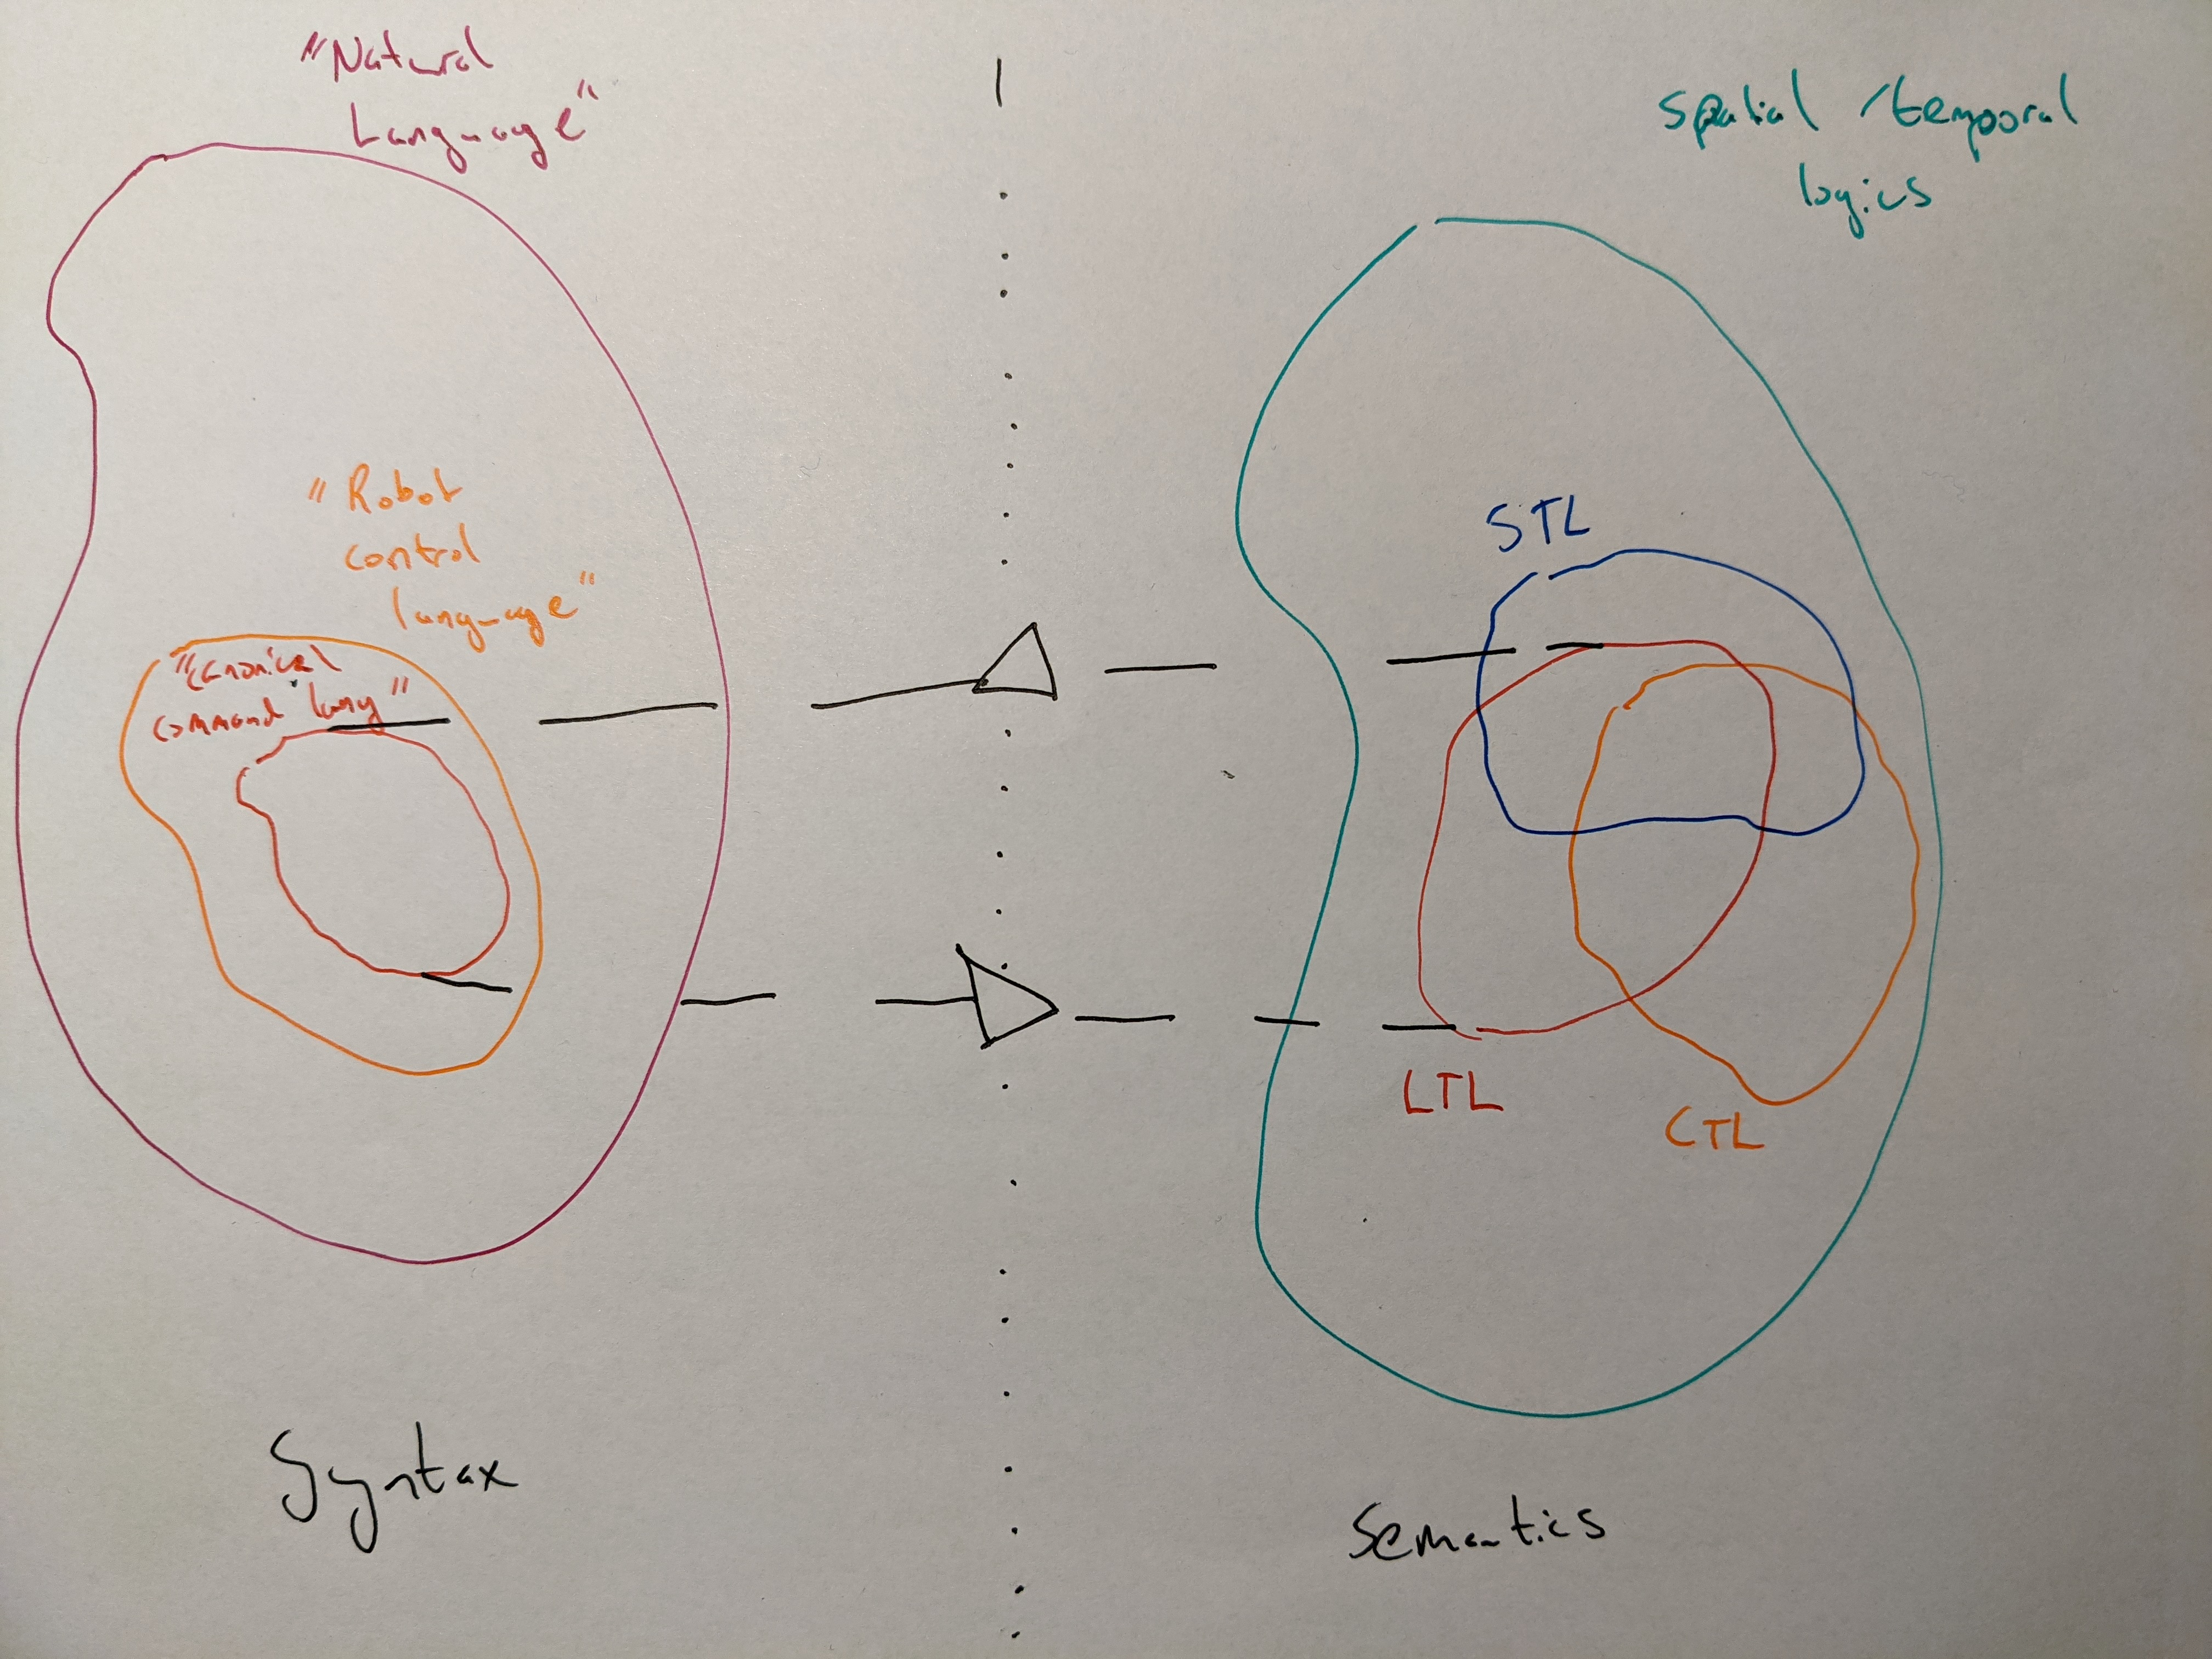
\includegraphics[width=150mm]{pics/one.jpg}
\caption{Language and Logical Spaces of Concern} \label{fig:M1}
\end{figure}

We begin in \autoref{fig:M1} with a high level overview of this semantic parsing
system, whereby the space of natural language syntax can be mapped to some
formal language semantic space (and possibly have some kind of inverse mapping).
We note that ``Natural Language'', while an idealized notion, can be thought of
the space of interpretable utterances. The relatively small subset of these
utterances which one might give to a robot, labeled ``Robot Control Language'',
is the ideal breadth our system would support, is still actually very large. We
therefore applying another filter, to the ``Canonical Command Language'' which
is inductively defined via some relatively thin set of grammar rules, which
simultaneously generate and parse expressions in some logic. Although we target
LTL because of its prominence in the literature and relatively straightforward
implementation and interpretation, it should be noted that their are other
temporal logics which may well be more expressive and better suited to the
actual problem of synthesizing controllers.

\begin{figure}
\centering
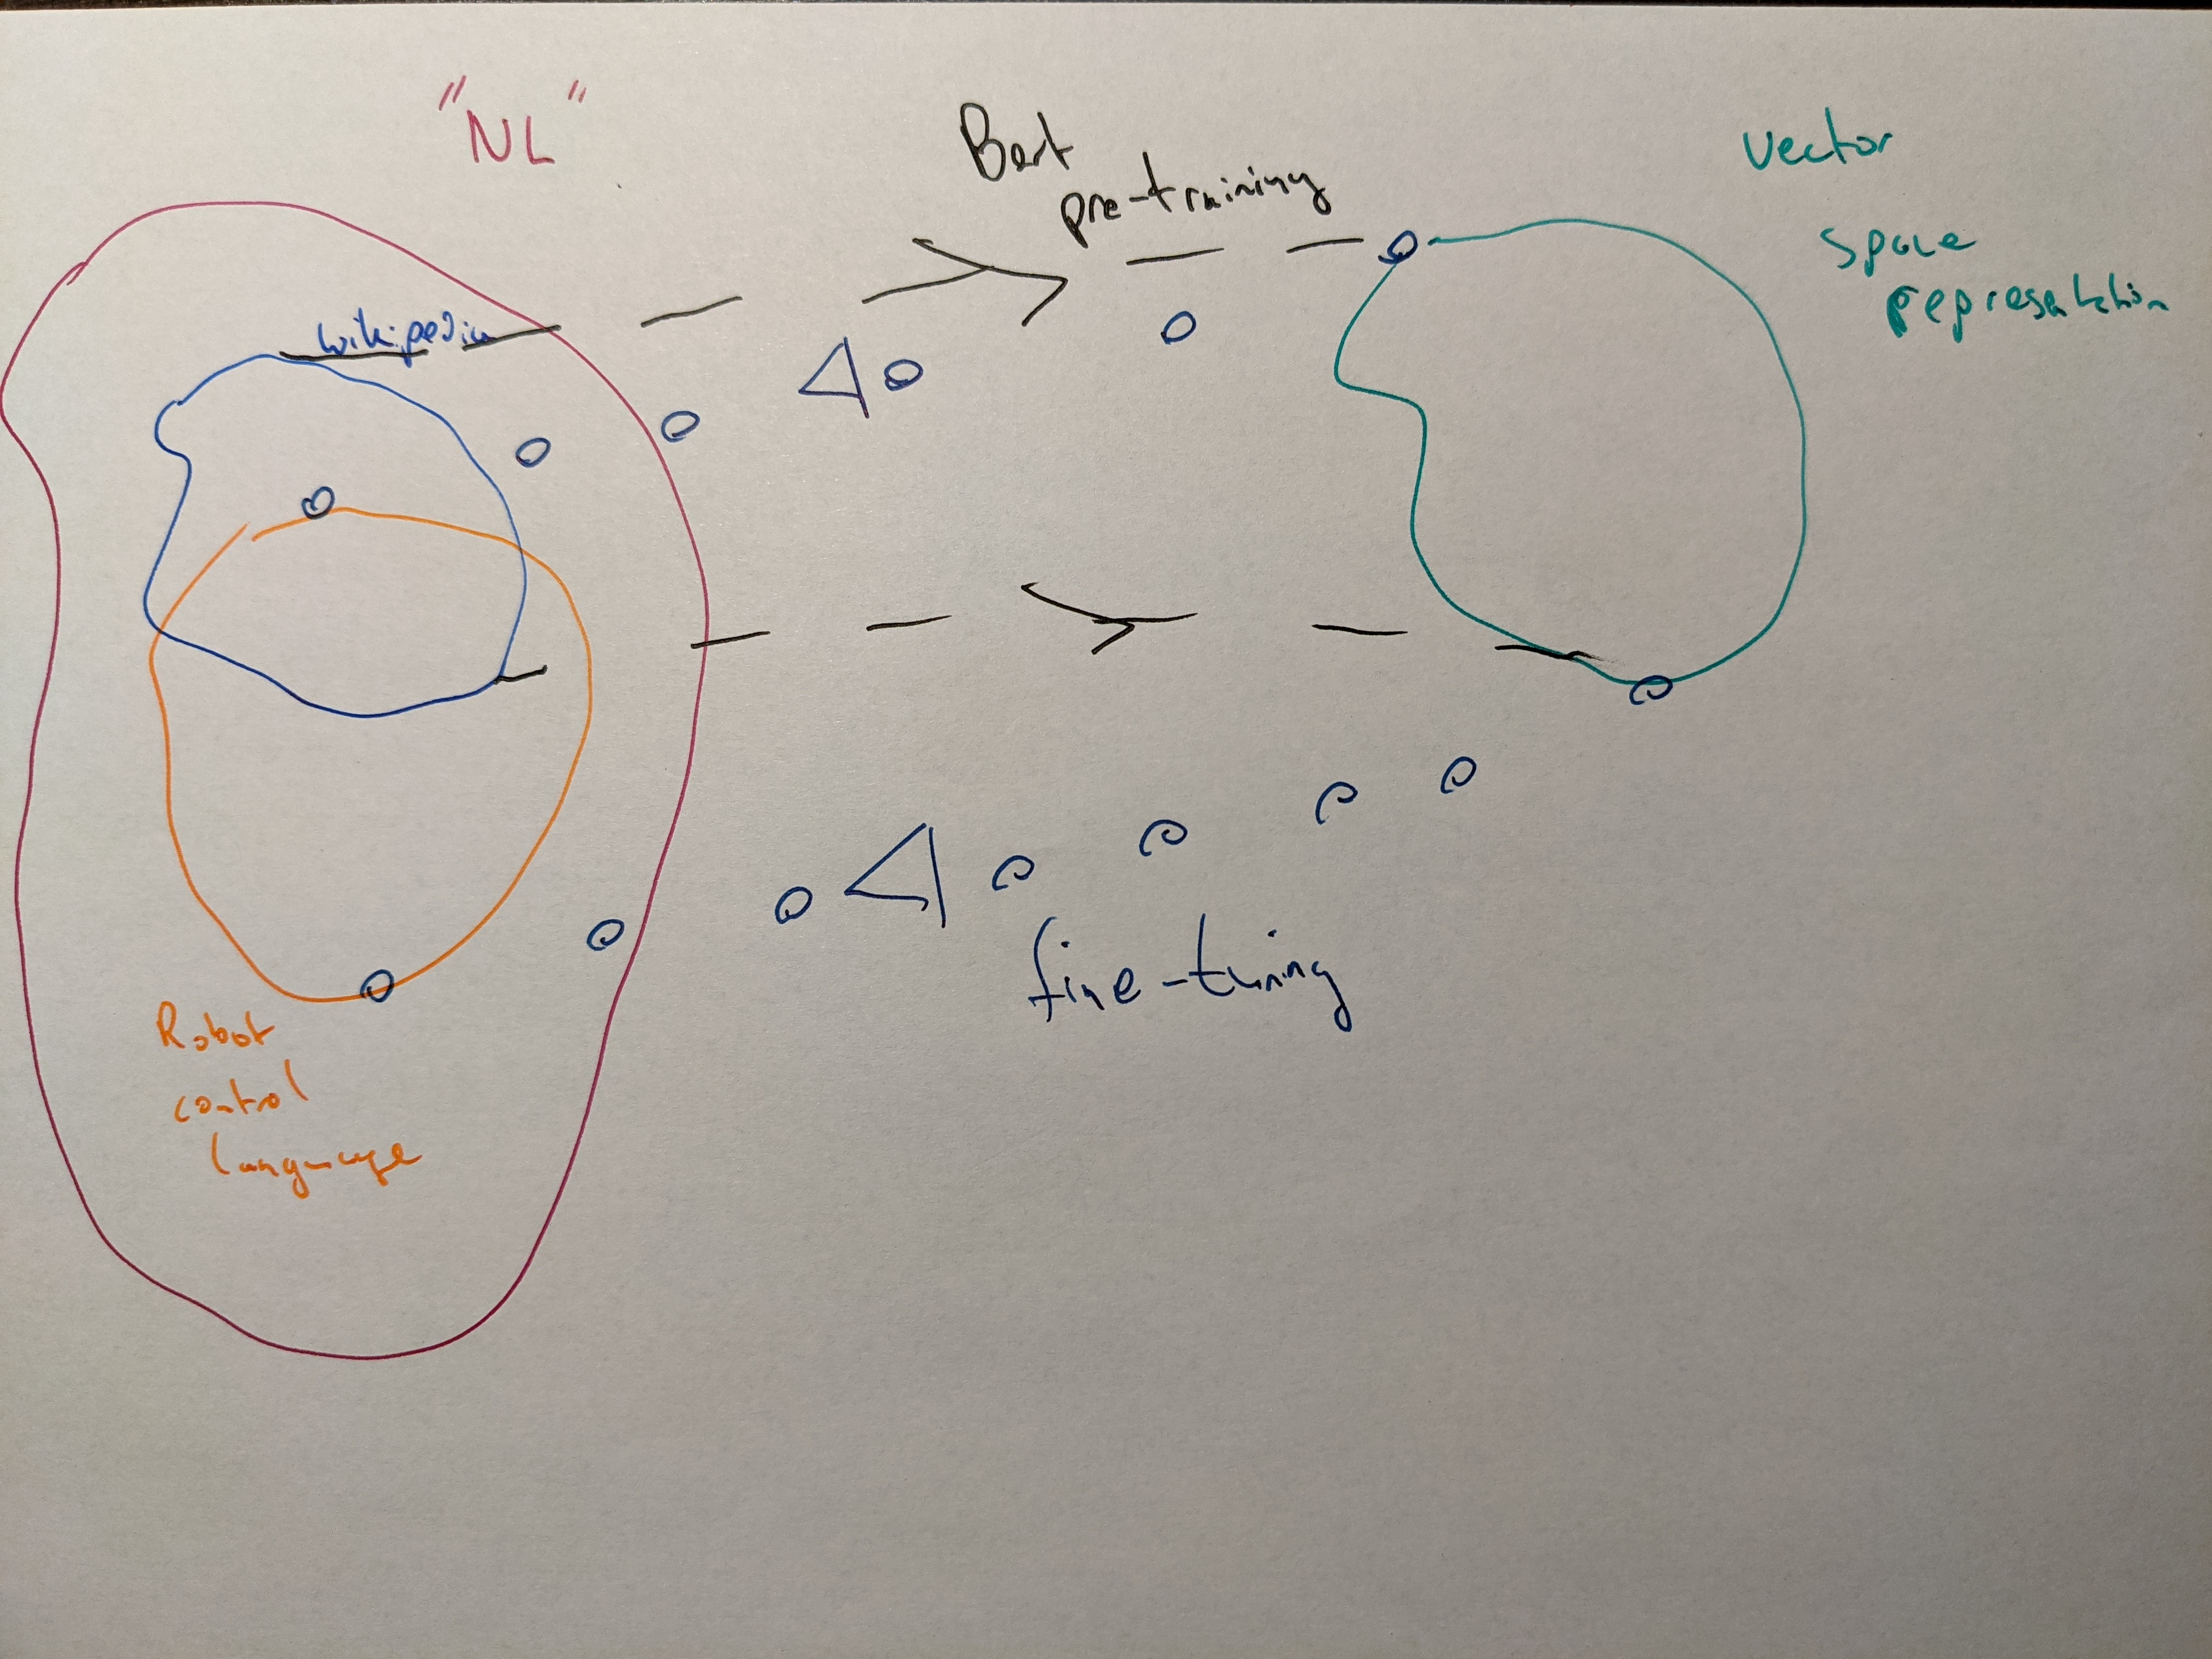
\includegraphics[width=150mm]{pics/two.jpg}
\caption{Transformer to Robot Control Language}\label{fig:M2}
\end{figure}

Due to the recent influx of transformer based language models like Bert and
GPT-3, we take for granted that the easiest way to target our ``Robot Control
Language'' will be through fine-tuning one of these models, as shown in
\autoref{fig:M2}. These transformers, trained on a separate corpus like
Wikepdia, can be mapped to some suitable set of robot commands, even though
these types of expressions will have a sparse presence in the corpus the model
was initially trained on (presumably Marco will know more about this than me).

In this context, we can then further refine the language to something less
natural, but more well-behaved. The whole proposed pipeline in \autoref{fig:M3},
indicates using the methodology as used in \cite{fewShotSem}, whereby the
semantic parser should ideally be able to take any command from the Robot
Control Language and turn it into a set of temporal logic formulas, distributed
according to most likely interpretation.

Ideally, the downstream dialogue system should either be able to ask for
clarification if two formulas are determined to be of some relative likelihood,
reject a formula that is not determined to be achievable (for whatever reason),
or synthesize a sequence of actions (and express those in the CNL) according to
the possibly modified current path.

\begin{figure}
\centering
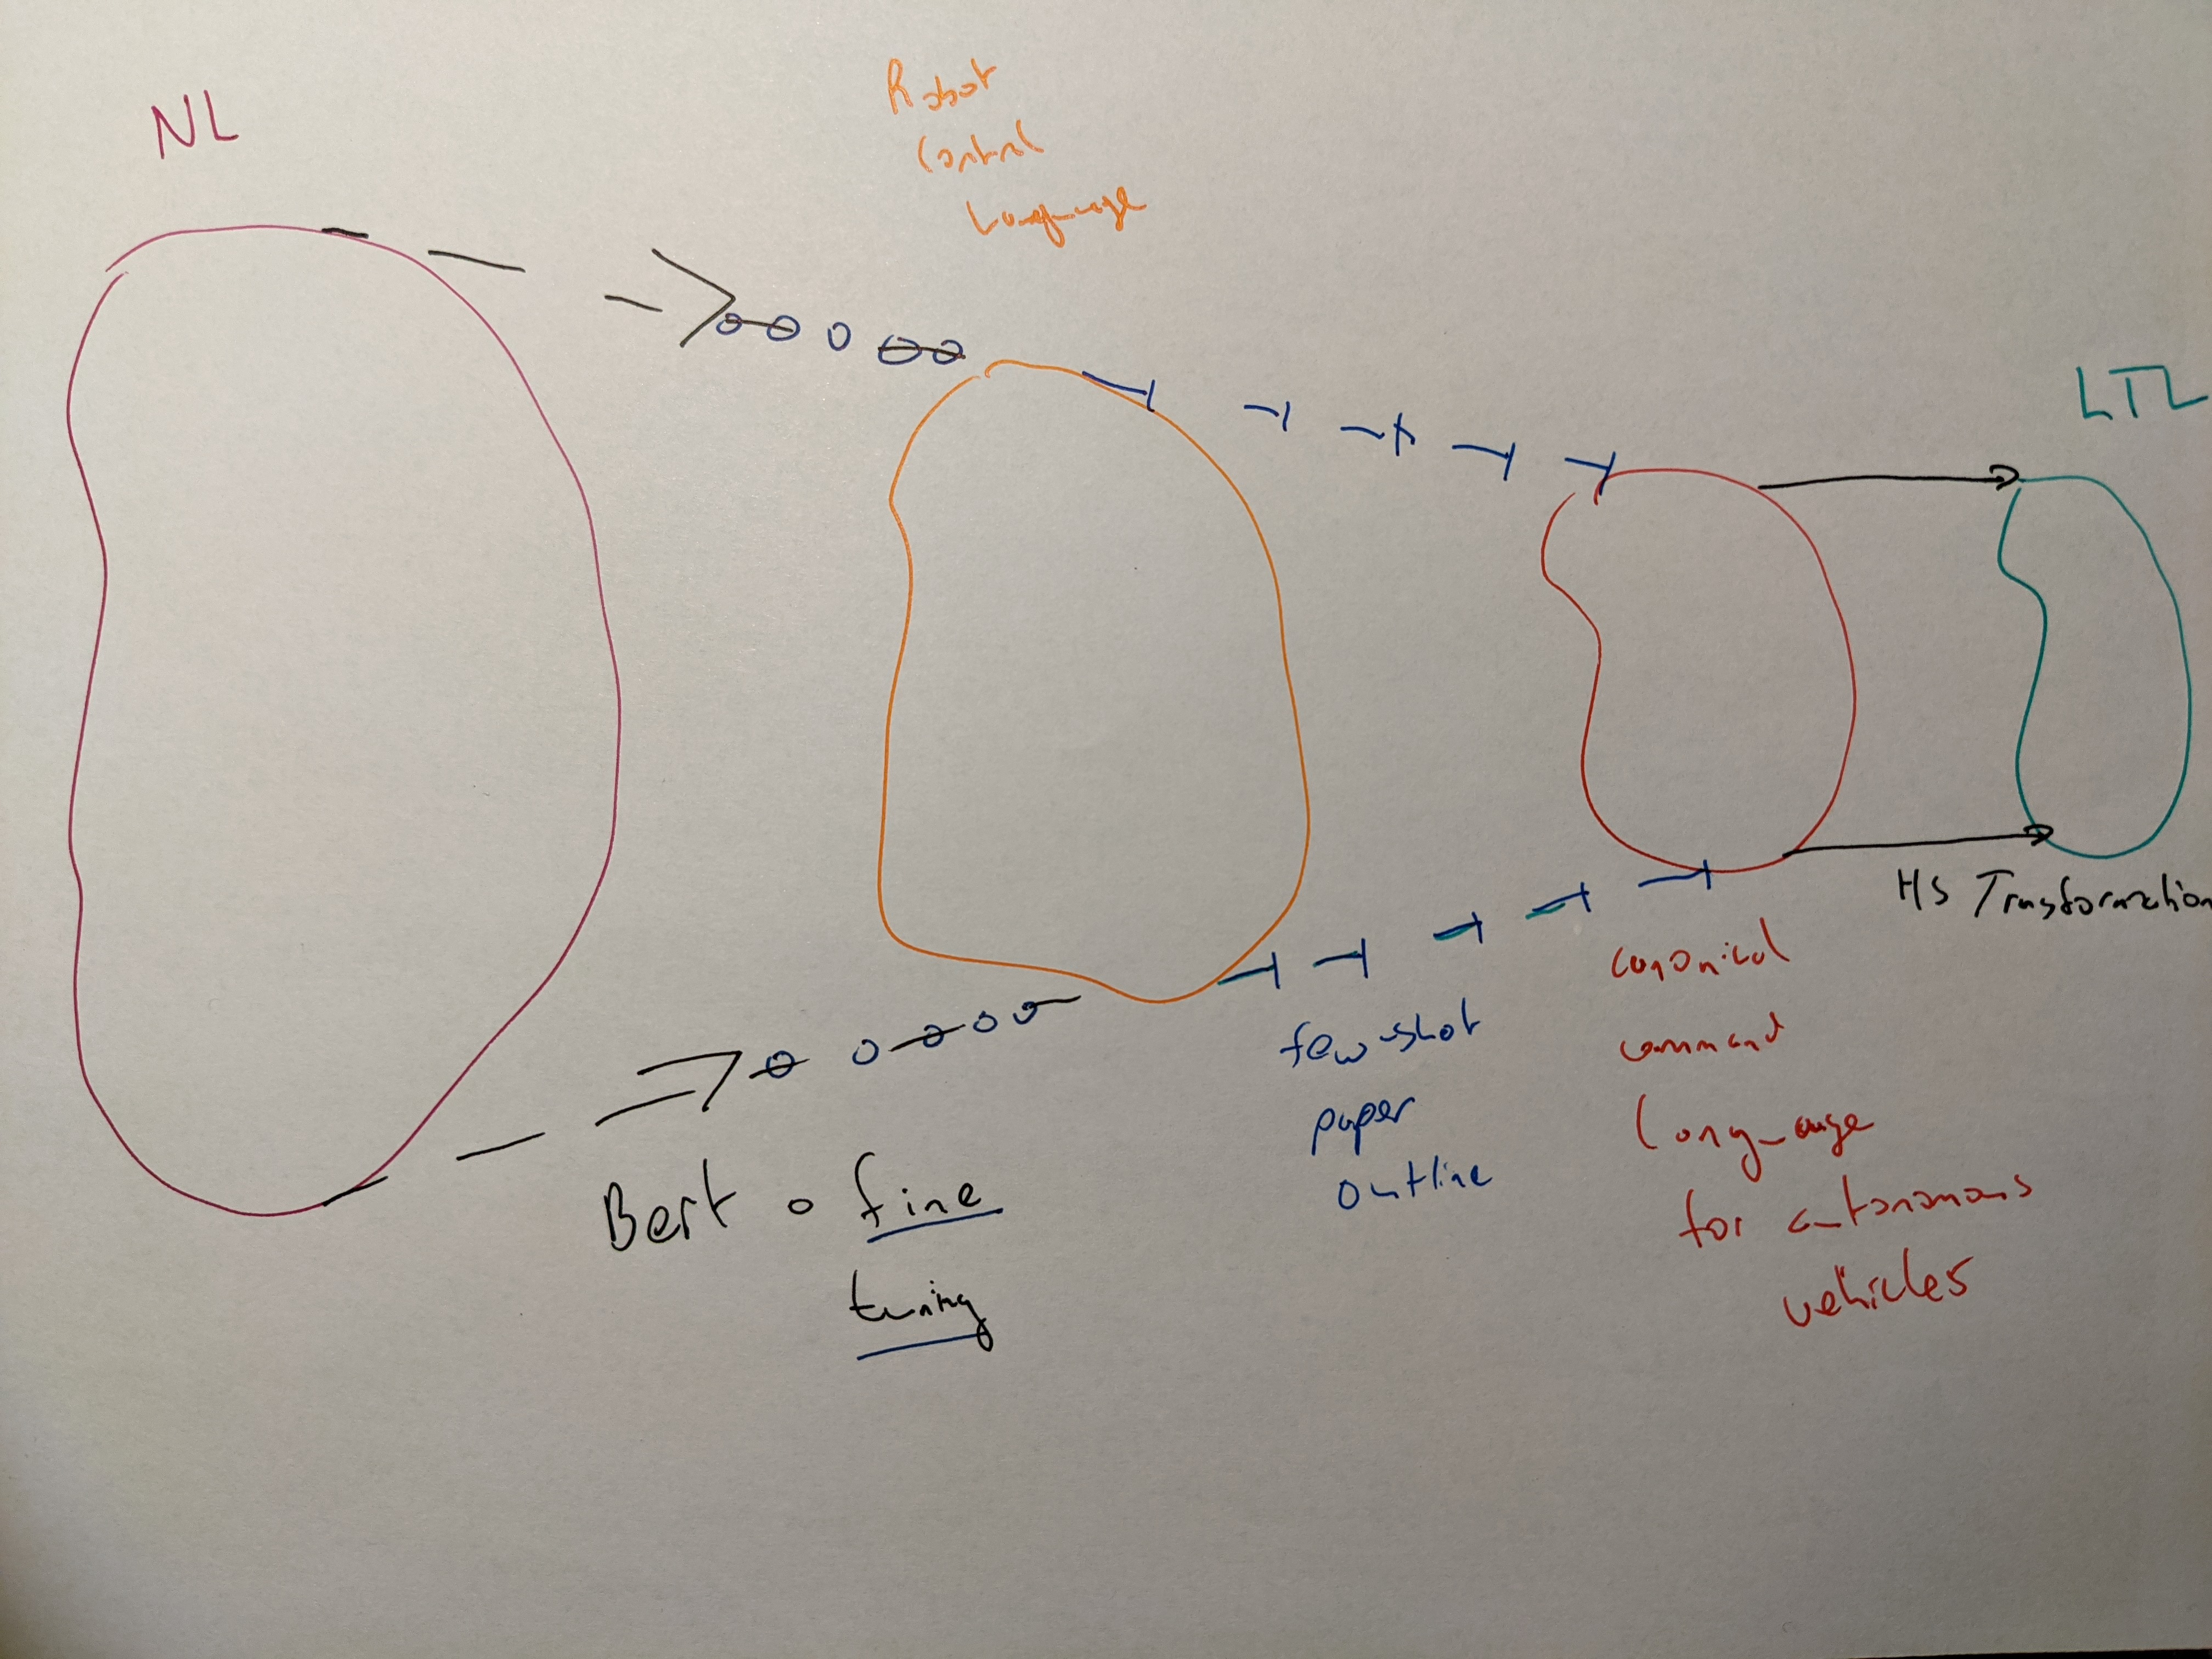
\includegraphics[width=150mm]{pics/three.jpg}
\caption{Pipeline from NL to LTL}\label{fig:M3}
\end{figure}

In theory, we can embed clauses which in turn reflect all of natural language :
``Stop at the man who is watching the tv show on his phone about time traveler
who goes back to the 12th century Mongolia, whereby the man, not speaking
Mongolian ...'' This is clearly outside the boundary of what the robot control
language should support, and ideally would be accepted or rejected by the
computer prior to the commands completion depending if there was a man looking
at a phone. Our parser currently accepts strings in our primitive canonical
language, designed in Grammatical Framework (GF), such as :

\begin{verbatim}
  p "drive to the store , turn right and stop at the dog"

  MultipleRoutes And (ConsPosCommand (SimpleCom (ModAction Drive (MkAdvPh To
  (WhichObject The Store)))) (BasePosCommand (SimpleCom (ModAction Turn
  (WherePhrase Right))) (SimpleCom (ModAction Stop (MkAdvPh At (WhichObject The
  Dog))))))
\end{verbatim}

However, we may envision our system being able to accept an expression in the
Robot Control Language like ``hit the petal till we reach the store, hang a
right, and halt when you see a cute little puppy''. We could certainly adjust
our parser to accomodate this, but it would be one of many possible edge cases
unlikely to be uttered. To accomodate many more such edge cases would cause an
exponential blowup in the parser size (thereby slowing down parsing), but more
importantly, cause the programmer a headache in building the parser, and then
mapping the NL ASTs to a LTL form. If we treat $F$ as the operating
expressing the existence a future state, $X$ as the next state, and $G$ meaning
the universal future, our desired LTL formula would most likely treat this as
$F\ (store \land\ (X\ turn\_right\ \land\ (F\ (G\ dog))))$, although we propose
that the actual grounding of these to images or controllable actions to some
downstream system.

LTL has been a popular logic for specifying controllable robot behaviors,
particularly with respect to verification of their behaviors. In
\cite{verifiedMotion}, Rizaldi et al. prove logical correctness of a motion
planner with respect to LTL formulas over maneuver automata formulas in the
Isabelle/HOL theorem prover, a non-dependent cousin of Agda.

They adopt a
modified semantics to \cite{fainekos2005temporal}, where they consider multiple
paths instead of one. They use a model checker to generate the plan

We are choosing to
deeply embed LTL in Agda for a few reasons, although the syntax of the embedding
could easily be translated to any other dependently typed theorem prover, and
with a little more effort probably any functional programming language. The
composition of a ``weakly verified'' natural language front-end with a formally
verified back-end such as in Rizaldi's work would pave the way for a fully
verified, utterance-to-vehicle-path pipeline for the autonomous vehicles.

The big question to address is what kind of verification conditions the natural
language component should be subjected to, and what kind of attacks would be
most important to preemptively anticipate. Substitution based attacks
\cite{substAttacks}, for instance, have been consistently emphasized throughout
our discussions so far. The question is, \emph{where} in the pipeline it would
be best to filter out the vulnerabilities, as well as \emph{how}.

One possibility would be to define words modulo equivalent meanings using
Wordnet \cite{wordnet} in the syntactic phase, either via training
\cite{ren-etal-2019-generating} (presumably during the fine-tuning to the Robot
Command Language or our ``canonicalization'' from that). It has been suggested
that Bert is already relatively robust against such attacks
\cite{hauser2021bert}, but we nonetheless feel that even higher sensitivities of
robustness may be better done at other phases in the pipeline.

Alternatively, one could just map these equivalent Wordnet forms to equivalent
parse trees using the Portable Grammar Format (PGF) Haskell library, which
essentially deeply embeds a GF grammar into a Generalized Algebraic Datatype
(GADT).

For instance, if we abstract over all abstract syntax trees for our grammar
using this library, we can define the following Haskell functions to equate a
``female human'' with a ``woman''.

\begin{verbatim}
treeMapfemalePersonIsWoman :: forall a. Tree a -> Tree a
treeMapfemalePersonIsWoman (GModObj GFemale GPerson) = GWoman
treeMapfemalePersonIsWoman GWoman                    = (GModObj GFemale GPerson)
treeMapfemalePersonIsWoman gp = composOp treeMapfemalePersonIsWoman gp
\end{verbatim}

There has been work integrating multiple language Wordnets with GF
\cite{virk2014developing}, so it would presumably be easy to integrate with our
system, depending on how large we want the grammar to get.


As it is unclear what the best direction for this is, and how the attacker model
in the context of an autonomous vehicle might work, all these decisions need to
be made in the context of discussions within the group.

[ Addendum before meeting : ]

The TOUCHDOWN data set \cite{chen2019touchdown} seems like the most
comprehensive and relevant data we'll find to fine-tune via one of these
pre-trained models. Please see https://github.com/lil-lab/touchdown


The idea of domain specific pre-training can be traced to
\cite{gururangan-etal-2020-dont}, where the authors introduce the concepts of
\emph{domain-adpative pretraining} and \emph{task-adpative pretraining}, whereby
this additional pre-training phase greatly improves efficacy of the LM on
corpus and task data not well represented in the training data.

The language models have been show \cite{bioBert}


\subsection{Syntax and Semantics}

When designing a grammar, we can pretend that initially

san abstract syntax, we have the following considerations

That when we are conditioning our syntacitc model of emperical, noisy, and
biased natural language data, so as to ideally generalize to unencountered
phenomena.

A central insight ambiguity :


\begin{itemize}
\item Ontological semantic space. What are we trying to represent?
\item Intended semantic space, the logical or formal system which our grammar
  will map to (via Haskell transformations)
\item  We want to account for some grammatical constructions via the abstract syntax, but
  outsource most of the grammaticality to the RGL
\item Data source. How to conform to the data set in a way that's faithful but
  doesn't overfit (the overfitting can probably result in generating functions
  which are useless and either make our parser slow down or overgenerate)
\end{itemize}

While theres no clear way of relating the trade-offs, we can come up with some
heuristics that shed light. Developing the ``ontological design'' allows one to
capture the intuitive problem.


\subsection{Ambiguity}

What happens when we encounter ambiguity? For instance, in p "go to the person
with the dog ." The prepositional phrase "with the dog" can either modify person
(as an adjectival clause) or it can modify go (as an adverbial clause). Because
the parser is designed to accommodate simple cases of both types of clauses,
these ambiguities, even in simple sentences from our corpus, will grow quickly.

In the case of a vehicle, however, knowing the correct parse is dependent on
the context in which the driver is going to the person : is the language
grounded in the fact that there a dog in the car, or a person in the purview
with a dog (or, most confusingly, perhaps both conditions are met, in which case
more contextual information is required to disambiguate the correct parse).

For we can actually program the semantics to accommodate both scenarios, whereby

$F (manwithdog /\ G Finish)$
$F (man /\ G Finish) /\ G withdog$

We can define our semantics to accommodate both interpretations, whereby the
parses produce unique semantic conditions, and the LTL solver will have to see
which condition is more easily satisfied. While this edge case may seem overly
pedantic to consider, as one's intuition might suggest the first case to be
overwhelmingly more natural, the


\section{Related Work}

\subsection{End-to-End Systems}

\subsubsection{Natural Language and LTL verification}


Just as important as producing a well-formed and meaningful LTL formula, but not
explored in our work, is the translation from a logical formula a trustworthy
controller meant for navigating a complex environment. For instance, in
\cite{plaku2016motion} the authors indicate how to actually ground basic
propositions from language to paths in a space, while our model, outputting
formulas with non-grounded base predicates, is merely concerned with logical
structure.

Similarly, in \cite{7759412}, the authors develop a Verifiable Distributed
Correspondence Graph (V-DCG) model whereby LTL formulas are used to ensure
grounded instruction sequences are consistent. This work builds on other work of
Kress-Gazit et al. \cite{provCorrectNatControl}, whereby the The Situated
Language Understanding Robot Platform (SLURP) allows translation of arbitrary
natural language into LTL. They suggest an ``ontology of common actions and the
type of formulas that they produce'' is of critical importance. Our work is
directly focused on the \emph{centrality of the grammar}, where a GF abstract
syntax design allows one to give a precise ontology. We therefore see our work as
a key intermediary phase when balancing formal and empirical interests.
Kress-Gazit's work is more concerned with the controllers generated as the end
result of a pipeline where the intermediary grammatical structure may not be so
relevant.

Our GF implementation, seeing the grammar as a necessary part of the
verifiability (in that we can systematically map our sequences of commands to
logical formulas representing sequences of states), also makes the possibility of
supporting multi-lingual verifiability more immediate. Our system does not
support this currently, but can easily be adjusted to so with the help of GF's
functors (roughly adapted from Standard ML's functors) and the RGL. The lack of wide-coverage
support of our grammar is possible to remediate through possible fine-tuning of
a large language model to a data-set which coheres to the language our GF
grammar generates, and we detail this in our discussion below [TODO : link].

Another approach seeks to train a natural language to LTL planner using both NNs
and reinforcement learning \cite{ltlSemParse}. Their work also uses a
simultaneous CFG to generate \emph{semantically inadequate} sentences with
corresponding LTL formulas from which they can direct machines to follow the
instructions, and then have users describe the robot behavior in a more natural
form. Despite this, their approach uses the machine to generate sentences and
corresponding situations, most of which are ``nonsense'' and need to be filtered
out, thereby leaving the narrations upon which their system leaves devoid of a
genuine empirical data source. In addition, their corpus only contains 266
words, still not the size one would need for our system. Finally, our suggested
use of a pre-trained language model fine-tuned to the semantic parsing task
gives us more flexibility in that the neural network and the verifiable grammar
and semantics in the kernel could allow us to focus on the problems of breadth
and depth somewhat independently.

The same group, in \cite{kuo2020deep}, explore the most general possible
end-to-end utterance to planner pipeline without intermediary states, namely, a
symbolic representation. While this ``cutting out the middle woman'' mentality
may be an idealistic long-term vision, it makes the system much too much of a
black box - even though they are able to reason about their system's behavior
through the use of attention maps. For the fine-tuned verification conditions
about the linguistic utterances our work explores, the intermediate symbolic
representations give a more explainable, predictable, and regulatable system.


Formal Requirements Elicitation Tool (Fret) {fret}

Use in aircraft, where there are many more controls, and the types of
descriptions are inherently much more ``structured'', i.e. the pilots are
assumed to have expertise and aren't just taking ad-hoc flights, but perhaps
still don't have engineering, verification, or logical knowledge to give precise
LTL specifications

In \cite{fret} they use the Prototype Verification System (PVS) theorem prover
to verify that

[Problem] There are two major challenges in making structured natural language
amenable to formal analysis: (1) associating requirements with formulas that can
be processed by analysis tools and (2) ensuring that the formulas conform to the
language semantics. \cite{fretish}

-----

\subsubsection{Theorem Provers and Verification for Robots}

In modeling work relating to route planning ideas into Agda, Hill et al.
~\cite{hillResource} have both designed a \emph{resource logic} interpreted a la
Curry-Howard in Agda. Subsequently they released  an agda formalization of
Planning Domain Definition Language (PDDL) ~\cite{hillAction}.

Since LTL is interperable in PDDL
~\cite{ltlPDDL}, and since our normal-form LTL formulas $F (\phi => F (\phi_0 => ... (G STOP)))$
, we can easily imagine the follow schema :

In ~\cite{planningForAV}, the authors indicate the need for the verification to
cover the full-spectrum, and that their are many approahces to planning, namely,
what they categorize as ``sequential, behavior-aware, and end-to-end'' planning.

[maybe add this to other section]
In this vision paper ~\cite{seshia2016towards}, the authors outline a few major
categories that need to be addressed to realize verification in AI,

\begin{itemize}
\item Formal Specification
\item Modeling Learning Systems
\item Scalable Design and Verification of Data and Models
\item Correct-by-Construction Methods
\end{itemize}

Environment (incl. Human) Modeling corresponds to Principles

In ~\cite{dreossiDS19} (recommending over the summer), the authors give a model of Adaptive Cruise Controllers (ACCs)

``We formulate this question as the falsification problem for CPS models with
ML components (CPSML): given a formal specification φ in signal temporal
logic (STL) [13], and a CPSML model M , find an input for which M does not
satisfy φ.''

The smaller the meaning space, the simpler the correct translation. This is of
obvious ewhen the meaning is interpreted as a formal system for a different
formal system, as is the case when studied in the context of programming
languages. When the formal meaning space attempts to capture an emperical,
non-formal system like natural language, the notion of correct translation is no
longer formally verifiable - it is ultimately up to human convenctions and
behaviors.

Logical specifications for Natural language
Past avoidance : Description
A condition has been ful-
filled in the past. This can give you a way of judging the success of a route (find the best route, and how well does the route follow this ideal route)



% Could ask Lapata in Edinburgh, whose work \cite{dong-lapata-2016-language}
%   is relevant and well-cited (although they use an encoder-decoder method)


\subsubsection{Tellex}

Stephanie Tellex has written extensively about natural language inputs and
interfaces with robots. Although she has not specifically written about
autonomous vehicles, the domains have enough intersection to warrant careful
consideration of much of her work, especially the recent stuff.

\begin{itemize}

\item Grounding with an intermediate symbolic state, no LTL, but possibly
 relevant for paper generally. She also cites \cite{walkTalk}, a seminal paper in this area
\begin{quote}
Instruction following is a supervised learning problem
where the agent must predict a trajectory that would satisfy an
input natural language command. \cite{tellexInstr}
\end{quote}
\item The review paper \cite{MARGE2022101255} making recommendations has a
 section on robustness, but this is mostly for the sake of allowing sharing of
 interfaces and efficacy, no mention of verification (which is what we're
 primarily after)
\item They design a NL -> LTL for drones that are grounded to actual landmarks \cite{9197068}
\item The group builds a trained pipeline that uses an object oriented
 template-instance methodology to generalize to different ontological
 categories in  \cite{hsiung2021generalizing} [under review]

\item In \cite{patellearning} build learn a semantic parser from NL to LTL (so
that the language is grounded) where they collect executions of the LTL formulas
in different environments using a weakly-supervised training method with
reinforcement learning Part if the paper has to do with the execution of the
command being dependent on the path taken by the robot executing the command,
not just meeting the goal requirements, thereby giving a complexity bonus in
comparison to previous work. She also evaluates the model on the \cite{walkTalk}
data set
\end{itemize}

\subsubsection{Commericial}

The public company Cerence \cite{} is already designing voice assistants for autonomous
vehicles, for which it has a large software stack between the voice processing
to actual control of current automative components. In addition to its
technologies, many of which aren't accessible to external researchers due to
intellectual property restrictions, Cerence has contracts with large automakers
[..]. It is therefore natural to inquire, what a small team with varied
backgrounds and not nearly the same expertise nor experience within the
technological team at Cerence can provide.

First, we believe that the focus on verification, insofar as we envision it, is
unlikely to be of current concern at Cerence due to the fact that their products
are still being developed, and the primary goal of producing a working product
is likely to precedence over preventing non-existent hostile actors.

\subsubsection{Alternative ideas}

While the evaluation of machine learning systems provides assurances using
different scores and metrics on different tasks assures one they may on average
perform better than humans at certain tasks, the advent of adversarial attacks
\cite{szegedy} with the intention of deceiving such a system by a hostile actor
leads the system designer to desire, and possible require additional
verification about the system's behavior. In the context of natural language
processing (NLP), where data sources rely on strings of text, these attacks can
focus an array of features from spellings of individual words to rearranging
entire sentences \cite{}. So-called synonym attacks, which adversarially target
the system at the lexical level, can cause traditional NLP models to [...]
\cite{}.


Aside from the user experience being compromised by a system which has been
adversarially afflicted, there is also a possibility of physical danger for the
passenger and other people in the vicinity. As voice directed robots have many
possible points of failure, we focus on two types of verification for our
system. Rather than focus on breadth of language coverage, which ML language
models excel at of due to their reliance on statistical modeling and tons
of data, our system is narrowly focused as a proof-of-concept, from which it
could either be extended by hand, or different components modified using
other techniques and tools.

TODO : other ml stuff, like ravi's publication

\section{Publications Description}

\subsection{Statistical (pre-trained) Language Models}


\begin{itemize}

\item In \cite{fewShotSem} [under review], the authors show how, using a \emph{synchronous
context-free grammar} (SCFG) to define a minified CNL with a parallel and dually
parsible semantic form, that one can use a large pre-trained language model as a front-end
to filter a much wider syntax into the CNL. GF's expressivity is
more expressive than the SCFG, at least based off a tertiary reading in the
index, and therefore if we carved out a subset of commands to cohere with our
LTL,

our model would be amenable to a similar

\item  \cite{hauser2021bert}  claims that Bert is robust, analyzing claims of four
 papers, including the one which uses a wordnet attack

\end{itemize}

\section{LTL Intro In Agda}
\section{LTL in Agda}




\section{LTL in Agda}

\begin{code}[hide]%
\>[0]\AgdaSymbol{\{-\#}\AgdaSpace{}%
\AgdaKeyword{OPTIONS}\AgdaSpace{}%
\AgdaPragma{--postfix-projections}\AgdaSpace{}%
\AgdaSymbol{\#-\}}\<%
\\
\>[0]\AgdaSymbol{\{-\#}\AgdaSpace{}%
\AgdaKeyword{OPTIONS}\AgdaSpace{}%
\AgdaPragma{--guardedness}\AgdaSpace{}%
\AgdaSymbol{\#-\}}\<%
\\
%
\\[\AgdaEmptyExtraSkip]%
\>[0]\AgdaKeyword{module}\AgdaSpace{}%
\AgdaModule{roadmap}\AgdaSpace{}%
\AgdaKeyword{where}\<%
\\
%
\\[\AgdaEmptyExtraSkip]%
\>[0]\AgdaKeyword{open}\AgdaSpace{}%
\AgdaKeyword{import}\AgdaSpace{}%
\AgdaModule{Data.Bool}\AgdaSpace{}%
\AgdaKeyword{renaming}\AgdaSpace{}%
\AgdaSymbol{(}\AgdaOperator{\AgdaFunction{\AgdaUnderscore{}∨\AgdaUnderscore{}}}\AgdaSpace{}%
\AgdaSymbol{to}\AgdaSpace{}%
\AgdaOperator{\AgdaFunction{\AgdaUnderscore{}∨'\AgdaUnderscore{}}}\AgdaSpace{}%
\AgdaSymbol{;}\AgdaSpace{}%
\AgdaOperator{\AgdaFunction{\AgdaUnderscore{}∧\AgdaUnderscore{}}}\AgdaSpace{}%
\AgdaSymbol{to}\AgdaSpace{}%
\AgdaOperator{\AgdaFunction{\AgdaUnderscore{}∧'\AgdaUnderscore{}}}\AgdaSymbol{)}\<%
\\
\>[0]\AgdaKeyword{open}\AgdaSpace{}%
\AgdaKeyword{import}\AgdaSpace{}%
\AgdaModule{Data.Nat}\AgdaSpace{}%
\AgdaKeyword{renaming}\AgdaSpace{}%
\AgdaSymbol{(}\AgdaOperator{\AgdaDatatype{\AgdaUnderscore{}≤\AgdaUnderscore{}}}\AgdaSpace{}%
\AgdaSymbol{to}\AgdaSpace{}%
\AgdaOperator{\AgdaDatatype{\AgdaUnderscore{}≤'\AgdaUnderscore{}}}\AgdaSpace{}%
\AgdaSymbol{;}\AgdaSpace{}%
\AgdaOperator{\AgdaFunction{\AgdaUnderscore{}<\AgdaUnderscore{}}}\AgdaSpace{}%
\AgdaSymbol{to}\AgdaSpace{}%
\AgdaOperator{\AgdaFunction{\AgdaUnderscore{}<'\AgdaUnderscore{}}}\AgdaSymbol{)}\<%
\\
\>[0]\AgdaComment{-- open import Data.Nat}\<%
\\
\>[0]\AgdaKeyword{open}\AgdaSpace{}%
\AgdaKeyword{import}\AgdaSpace{}%
\AgdaModule{Data.Unit}\AgdaSpace{}%
\AgdaKeyword{renaming}\AgdaSpace{}%
\AgdaSymbol{(}\AgdaRecord{⊤}\AgdaSpace{}%
\AgdaSymbol{to}\AgdaSpace{}%
\AgdaRecord{⊤'}\AgdaSymbol{)}\<%
\\
\>[0]\AgdaKeyword{open}\AgdaSpace{}%
\AgdaKeyword{import}\AgdaSpace{}%
\AgdaModule{Data.Empty}\AgdaSpace{}%
\AgdaKeyword{renaming}\AgdaSpace{}%
\AgdaSymbol{(}\AgdaDatatype{⊥}\AgdaSpace{}%
\AgdaSymbol{to}\AgdaSpace{}%
\AgdaDatatype{⊥'}\AgdaSymbol{)}\<%
\\
\>[0]\AgdaKeyword{open}\AgdaSpace{}%
\AgdaKeyword{import}\AgdaSpace{}%
\AgdaModule{Data.Sum}\<%
\\
\>[0]\AgdaKeyword{open}\AgdaSpace{}%
\AgdaKeyword{import}\AgdaSpace{}%
\AgdaModule{Relation.Nullary}\AgdaSpace{}%
\AgdaKeyword{renaming}\AgdaSpace{}%
\AgdaSymbol{(}\AgdaOperator{\AgdaFunction{¬\AgdaUnderscore{}}}\AgdaSpace{}%
\AgdaSymbol{to}\AgdaSpace{}%
\AgdaOperator{\AgdaFunction{¬'\AgdaUnderscore{}}}\AgdaSymbol{)}\<%
\\
\>[0]\AgdaKeyword{open}\AgdaSpace{}%
\AgdaKeyword{import}\AgdaSpace{}%
\AgdaModule{Data.Fin}\<%
\\
\>[0]\AgdaKeyword{open}\AgdaSpace{}%
\AgdaKeyword{import}\AgdaSpace{}%
\AgdaModule{Data.Product}\AgdaSpace{}%
\AgdaKeyword{using}\AgdaSpace{}%
\AgdaSymbol{(}\AgdaRecord{Σ}\AgdaSymbol{;}\AgdaSpace{}%
\AgdaOperator{\AgdaFunction{\AgdaUnderscore{}×\AgdaUnderscore{}}}\AgdaSymbol{;}\AgdaSpace{}%
\AgdaOperator{\AgdaInductiveConstructor{\AgdaUnderscore{},\AgdaUnderscore{}}}\AgdaSymbol{;}\AgdaSpace{}%
\AgdaField{proj₁}\AgdaSymbol{;}\AgdaSpace{}%
\AgdaField{proj₂}\AgdaSymbol{;}\AgdaSpace{}%
\AgdaFunction{∃}\AgdaSymbol{;}\AgdaSpace{}%
\AgdaFunction{Σ-syntax}\AgdaSymbol{;}\AgdaSpace{}%
\AgdaFunction{∃-syntax}\AgdaSymbol{)}\<%
\\
\>[0]\AgdaKeyword{open}\AgdaSpace{}%
\AgdaKeyword{import}\AgdaSpace{}%
\AgdaModule{Relation.Binary.PropositionalEquality}\<%
\\
%
\\[\AgdaEmptyExtraSkip]%
\>[0]\AgdaKeyword{module}\AgdaSpace{}%
\AgdaModule{Syntax}\AgdaSpace{}%
\AgdaSymbol{(}\AgdaBound{Atom}\AgdaSpace{}%
\AgdaSymbol{:}\AgdaSpace{}%
\AgdaPrimitive{Set}\AgdaSymbol{)}\AgdaSpace{}%
\AgdaKeyword{where}\<%
\end{code}

We briefly introduce Linear Temporal Logic (LTL), implemented in the Agda
theorem prover, intended for the reader unfamiliar with LTL, interactive theorem
provers, or both. Although there is a vast literature on temporal logics,
spanning logical theory, philosophical concerns, and applications, our
inroduction of the basic syntax and semantics in Agda will suggest a slightly
new perspective.

\subsection{Motivating LTL}

The primary ideas that we lean on are in motivating our formalazition are :

\begin{itemize}

%Theorem 2  There is an LTL model-checking algorithm whose running time depends linearly on the size of the Kripke structure and exponentially on
%the length of the LTL formula. MODELHANDBOOK

\item Motivated philosophically, LTL is captures, at least to some degree,
natural human intiution about temporal reasoning. That is, we hope that LTL is a
fair reflection of at least a subset of the temporal reasoning people carry out
without knowing any formal logic.

\item The semantical notion of model, and the behavior of a given stream of
actions taken by the system being modeled. A logical formula is given meaning by
relating it to some model abstracted from a physical system, and possibly a
trace of steps taken in that physical system.

\item LTL is decidable - that is, we can construct a model that validates an arbitrary formula or its
negation.

\item Model checking in LTL is decidable. The models are meant to be motivated
by real physical systems - in this case, the positions or velocity of a vehicle
relative to its local (and possibly global) environment - and whereby we want
our verifications of behaviors of this system to be systematically checkable
with automatically.

\item LTL can serve as template for more expressive or nuanced logical ideas. It
can be extended with more expressive notions of time as in Metric Temporal Logic
(MTL) and Signala Temporal Logick (STL) - or with other modalities to enable,
for instance, multiple interactive agents on the road.

\item LTL is, to first approximation, expressive enough for specifying commonly
encountered behaviors and specifications seen in the route and motion planning
domain

\item There are large number of well regarded and established model checkers
which could be adjoined to our definitions here. Adjacent to this, however, it
is a point of ongoing research ~\cite{appPf} to leverage Agda's dependent type system
and to internally decide the validity of a formula in a model.

\end{itemize}

The main point is that dual modalities in LTL quanitfying behaviors of
measurable events in time with regards to notions of \emph{some future time} and
\emph{all future times} admit a mathematically coherent theory in addition to
offering a philosophically interesting perspective on temporality, we can
leverage both the mathematical coherence and philosophical insight to offer
solutions to practical problems. In the sense that the philosophy of language is
concerned with how language is related to the world, we believe the and the
subset of natural language concerned with temporality generally, examined in the
use case of commanding a robot with deliberate intentionality in addition to
explicit expectation about the robots behavior, we may view this case study as an
intriguing place at the intersection of mathematics, computer science,
linguistics, and philosophy.

Despite model checking being a problem with high computational complexity
(relative to say, propisitional logic), our application for relatively simple
route planning don't require particularly large formulas. The complexity is
anticipated in the environment in which the vehicle operates, as well as the
natural language utterances used to describe and dictate the path through the
environment. The complexity of ensuring proper translations from natural
language (in addition to other components) is of a much bigger concern than
computational complextiy of model checking as here supposed. Because our haskell
translations produce normal forms that have a standard recursive nesting of
future F, and implications, rightarrow, we envision that the model checkers can
be heuristically adapted to handle larger formulas that may arise from randomly
generated LTL formulas.

A primary idea of temporal logics is that events, which may be abstract or
grounded in reality, take place sequentially in some axiomatizable notion of
time. Our everyday language captures this with notions of ``before'', ``after'',
``between'', ``forever'', ``later'', ``until'', and ``so-on and so-forth''. The
explicit notion of order (and causality) may be up to debate, as well as the
units by which time is measured, but LTL suppresses more complex notions of the
continuous time (at least from a computational view), as well as the branching
over possible worlds seen in Computation Tree Logic (CTL), simpifying assuptions
we'll accept for the time being. We complement this formalization with a simple
extension in a branched setting below, in large part to demonstrate that one can
be somewhat flexibile with the details once the basic infastructure is in place.

We base this formalization off Huth \& Ryan's introductory account in
\emph{LOGIC IN COMPUTER SCIENCE} CITEHERE. We shall contrast differences with
their presentation, with various pieces of our system as they arise.

The syntax of LTL is are formulas \blue{$\phi$} inductively defined type consists of

\begin{itemize}
\item Atomic events \green{atom} (which should ideally be grounded to reality), specified externally as some (presumably finite) type
\begin{itemize}
\item Atomic events could denote visible objects, sounds, or relative statements like ``being left'' when compared to some prior state
\end{itemize}
\item The standard propositional colletives for truthity, falsity, conjunction, disjunction, and negation :
  %\green{$\bottom$}
  %\green{$\top$}
  %\green{$\neg$}
\item Unary temporal operators representing
\begin{itemize}
\item the next state \green{$X$},
\item the existence of a future state \green{$F$},
\item the notion of henceforth, or forever \green{$G$}
\end{itemize}
\item Binary temporal operators representing
\begin{itemize}
\item The inclusive states in between two events next state \green{$U$},
\item weak until \green{$W$}
\item Release \green{$R$}
\end{itemize}
\end{itemize}

\begin{code}%
\>[0][@{}l@{\AgdaIndent{1}}]%
\>[2]\AgdaKeyword{data}\AgdaSpace{}%
\AgdaDatatype{ϕ}\AgdaSpace{}%
\AgdaSymbol{:}\AgdaSpace{}%
\AgdaPrimitive{Set}\AgdaSpace{}%
\AgdaKeyword{where}\<%
\\
\>[2][@{}l@{\AgdaIndent{0}}]%
\>[4]\AgdaComment{-- atom     : Fin n → ϕ instantiate with module instead}\<%
\\
%
\>[4]\AgdaInductiveConstructor{atom}%
\>[16]\AgdaSymbol{:}\AgdaSpace{}%
\AgdaBound{Atom}\AgdaSpace{}%
\AgdaSymbol{→}\AgdaSpace{}%
\AgdaDatatype{ϕ}\<%
\\
%
\>[4]\AgdaInductiveConstructor{⊥}\AgdaSpace{}%
\AgdaInductiveConstructor{⊤}%
\>[16]\AgdaSymbol{:}\AgdaSpace{}%
\AgdaDatatype{ϕ}\<%
\\
%
\>[4]\AgdaOperator{\AgdaInductiveConstructor{¬\AgdaUnderscore{}}}%
\>[16]\AgdaSymbol{:}\AgdaSpace{}%
\AgdaDatatype{ϕ}\AgdaSpace{}%
\AgdaSymbol{→}\AgdaSpace{}%
\AgdaDatatype{ϕ}\<%
\\
%
\>[4]\AgdaOperator{\AgdaInductiveConstructor{\AgdaUnderscore{}∨\AgdaUnderscore{}}}\AgdaSpace{}%
\AgdaOperator{\AgdaInductiveConstructor{\AgdaUnderscore{}∧\AgdaUnderscore{}}}\AgdaSpace{}%
\AgdaOperator{\AgdaInductiveConstructor{\AgdaUnderscore{}⇒\AgdaUnderscore{}}}\AgdaSpace{}%
\AgdaSymbol{:}\AgdaSpace{}%
\AgdaDatatype{ϕ}\AgdaSpace{}%
\AgdaSymbol{→}\AgdaSpace{}%
\AgdaDatatype{ϕ}\AgdaSpace{}%
\AgdaSymbol{→}\AgdaSpace{}%
\AgdaDatatype{ϕ}\<%
\\
%
\>[4]\AgdaInductiveConstructor{X}\AgdaSpace{}%
\AgdaInductiveConstructor{F}\AgdaSpace{}%
\AgdaInductiveConstructor{G}%
\>[16]\AgdaSymbol{:}\AgdaSpace{}%
\AgdaDatatype{ϕ}\AgdaSpace{}%
\AgdaSymbol{→}\AgdaSpace{}%
\AgdaDatatype{ϕ}\<%
\\
%
\>[4]\AgdaOperator{\AgdaInductiveConstructor{\AgdaUnderscore{}U\AgdaUnderscore{}}}\AgdaSpace{}%
\AgdaOperator{\AgdaInductiveConstructor{\AgdaUnderscore{}W\AgdaUnderscore{}}}\AgdaSpace{}%
\AgdaOperator{\AgdaInductiveConstructor{\AgdaUnderscore{}R\AgdaUnderscore{}}}\AgdaSpace{}%
\AgdaSymbol{:}\AgdaSpace{}%
\AgdaDatatype{ϕ}\AgdaSpace{}%
\AgdaSymbol{→}\AgdaSpace{}%
\AgdaDatatype{ϕ}\AgdaSpace{}%
\AgdaSymbol{→}\AgdaSpace{}%
\AgdaDatatype{ϕ}\<%
\end{code}
\begin{code}[hide]%
\>[0]\AgdaComment{-- power set}\<%
\\
\>[0]\AgdaFunction{𝑃}\AgdaSpace{}%
\AgdaSymbol{:}\AgdaSpace{}%
\AgdaPrimitive{Set}\AgdaSpace{}%
\AgdaSymbol{→}\AgdaSpace{}%
\AgdaPrimitive{Set}\<%
\\
\>[0]\AgdaFunction{𝑃}\AgdaSpace{}%
\AgdaBound{s}\AgdaSpace{}%
\AgdaSymbol{=}\AgdaSpace{}%
\AgdaBound{s}\AgdaSpace{}%
\AgdaSymbol{→}\AgdaSpace{}%
\AgdaDatatype{Bool}\<%
\\
%
\\[\AgdaEmptyExtraSkip]%
\>[0]\AgdaComment{-- 𝑃 Bool has four member}\<%
\\
\>[0]\AgdaComment{-- for example, we encode the empty set as follows}\<%
\\
\>[0]\AgdaFunction{empt}\AgdaSpace{}%
\AgdaSymbol{:}\AgdaSpace{}%
\AgdaFunction{𝑃}\AgdaSpace{}%
\AgdaDatatype{Bool}\<%
\\
\>[0]\AgdaFunction{empt}\AgdaSpace{}%
\AgdaInductiveConstructor{false}\AgdaSpace{}%
\AgdaSymbol{=}\AgdaSpace{}%
\AgdaInductiveConstructor{false}\<%
\\
\>[0]\AgdaFunction{empt}\AgdaSpace{}%
\AgdaInductiveConstructor{true}\AgdaSpace{}%
\AgdaSymbol{=}\AgdaSpace{}%
\AgdaInductiveConstructor{false}\<%
\end{code}

This syntacic form represents a weak boundary of this study, as the job of actually
determining how an atomic formula should pertain to reality can be best left to other
experts. Nonetheless, verifiability has been a primary pretext for this work,
and our development of the semantics of LTL demonstrate Agda's expressivitness,
elegance, and enforcement of correct-by-consturction programs. We proceed with defining the semantics.

Noting that a binary relation \blue{rel} is a higher type over a type $s$ - a
type of types indexed by two elements of $s$, we can then define the property of
a relation always being able to take another step. That is, for any element of
$s$, we can always construct a element $s'$ which it is related to by $r_s$,
that it always steps to.

\begin{code}%
\>[0]\AgdaFunction{rel}\AgdaSpace{}%
\AgdaSymbol{:}\AgdaSpace{}%
\AgdaPrimitive{Set}\AgdaSpace{}%
\AgdaSymbol{→}\AgdaSpace{}%
\AgdaPrimitive{Set₁}\<%
\\
\>[0]\AgdaFunction{rel}\AgdaSpace{}%
\AgdaBound{s}\AgdaSpace{}%
\AgdaSymbol{=}\AgdaSpace{}%
\AgdaBound{s}\AgdaSpace{}%
\AgdaSymbol{→}\AgdaSpace{}%
\AgdaBound{s}\AgdaSpace{}%
\AgdaSymbol{→}\AgdaSpace{}%
\AgdaPrimitive{Set}\<%
\\
%
\\[\AgdaEmptyExtraSkip]%
\>[0]\AgdaFunction{relAlwaysSteps}\AgdaSpace{}%
\AgdaSymbol{:}\AgdaSpace{}%
\AgdaSymbol{\{}\AgdaBound{S}\AgdaSpace{}%
\AgdaSymbol{:}\AgdaSpace{}%
\AgdaPrimitive{Set}\AgdaSymbol{\}}\AgdaSpace{}%
\AgdaSymbol{→}\AgdaSpace{}%
\AgdaFunction{rel}\AgdaSpace{}%
\AgdaBound{S}\AgdaSpace{}%
\AgdaSymbol{→}\AgdaSpace{}%
\AgdaPrimitive{Set}\<%
\\
\>[0]\AgdaFunction{relAlwaysSteps}\AgdaSpace{}%
\AgdaSymbol{\{}\AgdaBound{S}\AgdaSymbol{\}}\AgdaSpace{}%
\AgdaBound{rₛ}\AgdaSpace{}%
\AgdaSymbol{=}\AgdaSpace{}%
\AgdaSymbol{∀}\AgdaSpace{}%
\AgdaSymbol{(}\AgdaBound{s}\AgdaSpace{}%
\AgdaSymbol{:}\AgdaSpace{}%
\AgdaBound{S}\AgdaSymbol{)}\AgdaSpace{}%
\AgdaSymbol{→}\AgdaSpace{}%
\AgdaFunction{Σ[}\AgdaSpace{}%
\AgdaBound{s'}\AgdaSpace{}%
\AgdaFunction{∈}\AgdaSpace{}%
\AgdaBound{S}\AgdaSpace{}%
\AgdaFunction{]}\AgdaSpace{}%
\AgdaSymbol{(}\AgdaBound{rₛ}\AgdaSpace{}%
\AgdaBound{s}\AgdaSpace{}%
\AgdaBound{s'}\AgdaSymbol{)}\<%
\end{code}

The dichotomous position about the epistemological status of logic, whether
logical knowledge is primarily about inference, in the proof theoretic
traditions, or truth, in the model theoretic traditions, can be both juxtaposed
and illuminated through our work here.

Theorem provers have often promote ``syntactic view'' of logic, with programs
and proof derivations taking primacy in interactive theorem provers like Agda
due to the undecidable notion of generating a proof object for a given type.

The ``semantic view'' is much more well esablished in the verification
community, where model checkers, whose primary notion is of ``a model'', and
what the feasibility, or truth, of a piece of syntax means relative to at least
some models.

We now define this fundamental notion of \emph{model} and
interpret it in our temporal setting. When used for arbitrary modalities, we
call a model a \emph{Kripke Structure}, and it can be seen as a fundamental
example of a general transition system, namely, a Kripke Structure a state-labeled. Used
colloquially, a model represents an approximation of a complicated system with
simpler and more understandable subsystem. Since a model is an abstraction which
involves simplifying assumptions, it may only be faithful to certain behaviors
of the system it is trying to capture and, indeed, may contradict others.

Given some atomic propositions (groundable to reality) a model \blue{$M$} in LTL consists
of a

\begin{itemize}
\item Type of states, \pink{State} TODO : fix colors
\item A binary relation, or step function over, those states, \pink{$\hookrightarrow$}
\item Evidence that the relation always can take a step or that we can't get into a stuck state, \pink{relSteps}
\begin{itemize}
\item We note that this condition can be dropped for our purposes, noting that including it simply makes our definition of model a subtype off a more general notion, whereby almost all of our code below foregoes using it
\end{itemize}
\item A labeling function, L, which determines the atomic propositions true at a given state
\end{itemize}

\begin{code}%
\>[0]\AgdaKeyword{record}\AgdaSpace{}%
\AgdaRecord{𝑀}\AgdaSpace{}%
\AgdaSymbol{(}\AgdaBound{Atom}\AgdaSpace{}%
\AgdaSymbol{:}\AgdaSpace{}%
\AgdaPrimitive{Set}\AgdaSymbol{)}\AgdaSpace{}%
\AgdaSymbol{:}\AgdaSpace{}%
\AgdaPrimitive{Set₁}\AgdaSpace{}%
\AgdaKeyword{where}\<%
\\
\>[0][@{}l@{\AgdaIndent{0}}]%
\>[2]\AgdaKeyword{field}\<%
\\
\>[2][@{}l@{\AgdaIndent{0}}]%
\>[4]\AgdaField{State}\AgdaSpace{}%
\AgdaSymbol{:}\AgdaSpace{}%
\AgdaPrimitive{Set}\<%
\\
%
\>[4]\AgdaOperator{\AgdaField{\AgdaUnderscore{}↪\AgdaUnderscore{}}}\AgdaSpace{}%
\AgdaSymbol{:}\AgdaSpace{}%
\AgdaFunction{rel}\AgdaSpace{}%
\AgdaField{State}\<%
\\
%
\>[4]\AgdaField{relSteps}\AgdaSpace{}%
\AgdaSymbol{:}\AgdaSpace{}%
\AgdaFunction{relAlwaysSteps}\AgdaSpace{}%
\AgdaOperator{\AgdaField{\AgdaUnderscore{}↪\AgdaUnderscore{}}}\<%
\\
%
\>[4]\AgdaComment{-- L : State → 𝑃 Atom}\<%
\\
%
\>[4]\AgdaField{L}\AgdaSpace{}%
\AgdaSymbol{:}\AgdaSpace{}%
\AgdaField{State}\AgdaSpace{}%
\AgdaSymbol{→}\AgdaSpace{}%
\AgdaBound{Atom}\AgdaSpace{}%
\AgdaSymbol{→}\AgdaSpace{}%
\AgdaPrimitive{Set}\<%
\end{code}


We note that in the textbook treatment, the labeling function provides a subset
of the set of atoms for any given state state, that the codomain of the labeller
is the powerset of the atomic propositions. We opt instead to see the labeling
function as a type indexed by states and atoms. This typed formulation provides
not only a convenience for dealing with certain beuracracies encountered using
the classical power set formulation, but allows us to forego so-called ``Boolean
Blindness'' ~\cite{harperBlindness} and have proof objects which whose syntax
more expressively represents the arguments. To see further how one can represent
various set-theoretic notions in Agda, and familiarize oneself with the
type-level thinking which so naturally avoids boolean myopia, please see TODO :
Section in the standard library.

With a model defined, we next establish the fundamental notion of a path in a
model - which is the primary ingredient to establish how a formula can be
evaluated relative to sequence of events in a model. More explicitly, paths
allow us to represent time, and they should be seen as discrete signals
dependent upon the type of state chosen. This intuition actually manifests in
Metric Temrpoal Logic (MTL) and Signal Temporal Logic (STL), which generalizes
temporal logic to transition systems which are actually just signals with a
real-time domains.

In the discrete case, the formulation of a path is also subject to how one
interprets the infinte sequence of states over which our temporal expressions
(and intuitions) take place. We can interpret an infinite sequence manifesting
via two possible definitions

\begin{itemize}
\item The coinductive type of streams over states, as done in ~\cite{coqLTL}.
\item The mathematicians view of a sequence, that is the set of states indexed
by the natural numbers.
\end{itemize}

Given a model defined in the context of some atoms, we first outline the stream
approach. A stream, often analagously referenced as an ``infinite list'', is
given by a piece of visibile data, the head, \pink{hd}, and the tail, \pink{tl},
which is just a corecursive reference to another list whose data will be
accessible later when it is \emph{needed}. Streams are a fundamental datatype
in the call-by-name operational semantics, whereby lazy evaluation allows one to
defer computing on the tail until it is needed, and this makes perfect sense if
one interprets a stream as a discretized version continuous signal which we may
occassionally sample.

\begin{code}[hide]%
\>[0]\AgdaKeyword{module}\AgdaSpace{}%
\AgdaModule{Transition}\AgdaSpace{}%
\AgdaSymbol{(}\AgdaBound{Atom}\AgdaSpace{}%
\AgdaSymbol{:}\AgdaSpace{}%
\AgdaPrimitive{Set}\AgdaSymbol{)}\AgdaSpace{}%
\AgdaSymbol{(}\AgdaBound{Model}\AgdaSpace{}%
\AgdaSymbol{:}\AgdaSpace{}%
\AgdaRecord{𝑀}\AgdaSpace{}%
\AgdaBound{Atom}\AgdaSymbol{)}\AgdaSpace{}%
\AgdaKeyword{where}\<%
\\
\>[0][@{}l@{\AgdaIndent{0}}]%
\>[2]\AgdaKeyword{open}\AgdaSpace{}%
\AgdaModule{Syntax}\AgdaSpace{}%
\AgdaBound{Atom}\AgdaSpace{}%
\AgdaKeyword{public}\<%
\\
%
\>[2]\AgdaKeyword{open}\AgdaSpace{}%
\AgdaModule{𝑀}\AgdaSpace{}%
\AgdaBound{Model}\<%
\end{code}
\begin{code}%
%
\>[2]\AgdaKeyword{record}\AgdaSpace{}%
\AgdaRecord{Stream}\AgdaSpace{}%
\AgdaSymbol{:}\AgdaSpace{}%
\AgdaPrimitive{Set}\AgdaSpace{}%
\AgdaKeyword{where}\<%
\\
\>[2][@{}l@{\AgdaIndent{0}}]%
\>[4]\AgdaKeyword{coinductive}\<%
\\
%
\>[4]\AgdaKeyword{field}\<%
\\
\>[4][@{}l@{\AgdaIndent{0}}]%
\>[6]\AgdaField{hd}\AgdaSpace{}%
\AgdaSymbol{:}\AgdaSpace{}%
\AgdaField{State}\<%
\\
%
\>[6]\AgdaField{tl}\AgdaSpace{}%
\AgdaSymbol{:}\AgdaSpace{}%
\AgdaRecord{Stream}\<%
\end{code}
\begin{code}[hide]%
%
\>[2]\AgdaKeyword{open}\AgdaSpace{}%
\AgdaModule{Stream}\<%
\end{code}

To define a path, \blue{Path}, in a model, we need an inifinite sequence of
states \pink{$infSeq$} that don't reach a stuck, or deadlocked state with
regards to some given structure - we want \pink{$infSeq$} to always transition.
We say that the stream always transitions when the first two elements are
related by the model's step function \pink{$\hookrightarrow$}, as evidenced by
\pink{headValid} and we can coinductively prove this for the tail of the stream,
\pink{tailValid}. The second state, \blue{nextState} of a stream is defined by taking
the head of the tail of the stream.

\begin{code}%
%
\>[2]\AgdaFunction{nextState}\AgdaSpace{}%
\AgdaSymbol{:}\AgdaSpace{}%
\AgdaRecord{Stream}\AgdaSpace{}%
\AgdaSymbol{→}\AgdaSpace{}%
\AgdaField{State}\<%
\\
%
\>[2]\AgdaFunction{nextState}\AgdaSpace{}%
\AgdaBound{s}\AgdaSpace{}%
\AgdaSymbol{=}\AgdaSpace{}%
\AgdaField{hd}\AgdaSpace{}%
\AgdaSymbol{(}\AgdaField{tl}\AgdaSpace{}%
\AgdaBound{s}\AgdaSymbol{)}\<%
\\
%
\\[\AgdaEmptyExtraSkip]%
%
\>[2]\AgdaKeyword{record}\AgdaSpace{}%
\AgdaRecord{streamAlwaysTransitions}\AgdaSpace{}%
\AgdaSymbol{(}\AgdaBound{stream}\AgdaSpace{}%
\AgdaSymbol{:}\AgdaSpace{}%
\AgdaRecord{Stream}\AgdaSymbol{)}\AgdaSpace{}%
\AgdaSymbol{:}\AgdaSpace{}%
\AgdaPrimitive{Set}\AgdaSpace{}%
\AgdaKeyword{where}\<%
\\
\>[2][@{}l@{\AgdaIndent{0}}]%
\>[4]\AgdaKeyword{coinductive}\<%
\\
%
\>[4]\AgdaKeyword{field}\<%
\\
\>[4][@{}l@{\AgdaIndent{0}}]%
\>[6]\AgdaField{headValid}\AgdaSpace{}%
\AgdaSymbol{:}\AgdaSpace{}%
\AgdaField{hd}\AgdaSpace{}%
\AgdaBound{stream}\AgdaSpace{}%
\AgdaOperator{\AgdaField{↪}}\AgdaSpace{}%
\AgdaFunction{nextState}\AgdaSpace{}%
\AgdaBound{stream}\<%
\\
%
\>[6]\AgdaField{tailValid}\AgdaSpace{}%
\AgdaSymbol{:}\AgdaSpace{}%
\AgdaRecord{streamAlwaysTransitions}\AgdaSpace{}%
\AgdaSymbol{(}\AgdaField{tl}\AgdaSpace{}%
\AgdaBound{stream}\AgdaSymbol{)}\<%
\\
%
\\[\AgdaEmptyExtraSkip]%
%
\>[2]\AgdaKeyword{record}\AgdaSpace{}%
\AgdaRecord{Path}\AgdaSpace{}%
\AgdaSymbol{:}\AgdaSpace{}%
\AgdaPrimitive{Set}\AgdaSpace{}%
\AgdaKeyword{where}\<%
\\
\>[2][@{}l@{\AgdaIndent{0}}]%
\>[4]\AgdaKeyword{field}\<%
\\
\>[4][@{}l@{\AgdaIndent{0}}]%
\>[6]\AgdaField{infSeq}%
\>[21]\AgdaSymbol{:}\AgdaSpace{}%
\AgdaRecord{Stream}\<%
\\
%
\>[6]\AgdaField{isTransitional}\AgdaSpace{}%
\AgdaSymbol{:}\AgdaSpace{}%
\AgdaRecord{streamAlwaysTransitions}\AgdaSpace{}%
\AgdaField{infSeq}\<%
\end{code}
\begin{code}[hide]%
%
\>[2]\AgdaKeyword{open}\AgdaSpace{}%
\AgdaModule{streamAlwaysTransitions}\<%
\\
%
\>[2]\AgdaKeyword{open}\AgdaSpace{}%
\AgdaModule{Path}\<%
\end{code}

While a model's step relation may allow more than one possible state that a
given state can transition to, a path restricts this relation to be a function :
it gives us the one and only one transition we can make, and gurantees that
there is no sequence of states for which a possible intermediary transition is
absent. The ability to quantify over possible paths from a given state is the
branching referenced in CTL.

As paths not only contain streams of states, but also are forced to cohere with
the model's step relation, we define two helper functions to overload the head
and tail operations of the path's stream onto to the path itself.

\begin{code}%
%
\>[2]\AgdaFunction{headPath}\AgdaSpace{}%
\AgdaSymbol{:}\AgdaSpace{}%
\AgdaRecord{Path}\AgdaSpace{}%
\AgdaSymbol{→}\AgdaSpace{}%
\AgdaField{State}\<%
\\
%
\>[2]\AgdaFunction{headPath}\AgdaSpace{}%
\AgdaBound{x}\AgdaSpace{}%
\AgdaSymbol{=}\AgdaSpace{}%
\AgdaField{hd}\AgdaSpace{}%
\AgdaSymbol{(}\AgdaField{infSeq}\AgdaSpace{}%
\AgdaBound{x}\AgdaSymbol{)}\<%
\\
%
\\[\AgdaEmptyExtraSkip]%
%
\>[2]\AgdaFunction{tailPath}\AgdaSpace{}%
\AgdaSymbol{:}\AgdaSpace{}%
\AgdaRecord{Path}\AgdaSpace{}%
\AgdaSymbol{→}\AgdaSpace{}%
\AgdaRecord{Path}\<%
\\
%
\>[2]\AgdaFunction{tailPath}\AgdaSpace{}%
\AgdaBound{p}\AgdaSpace{}%
\AgdaSymbol{.}\AgdaField{infSeq}%
\>[29]\AgdaSymbol{=}\AgdaSpace{}%
\AgdaField{tl}\AgdaSpace{}%
\AgdaSymbol{(}\AgdaField{infSeq}\AgdaSpace{}%
\AgdaBound{p}\AgdaSymbol{)}\<%
\\
%
\>[2]\AgdaFunction{tailPath}\AgdaSpace{}%
\AgdaBound{p}\AgdaSpace{}%
\AgdaSymbol{.}\AgdaField{isTransitional}\AgdaSpace{}%
\AgdaSymbol{=}\AgdaSpace{}%
\AgdaField{tailValid}\AgdaSpace{}%
\AgdaSymbol{(}\AgdaField{isTransitional}\AgdaSpace{}%
\AgdaBound{p}\AgdaSymbol{)}\<%
\end{code}


\subsection{Sequential Definition}

We now contrast this utilizing the mathematicians view of a sequence, that is,
we bypass the coinductive stream and assert that the structure of the path is
given my a map ℕ → State. We then adjust our definition of the propery of
deadlock freedom. The \blue{alwaysSteps} function says that, given a sequence of
states $s$, $s_i$ steps to $s_{i+1}$ for any number $i$. Again, this is all
relative to some given model $M$. Although the seqence formulated as a function
and a stream look quite different, we prove they are isomorphic elsewhere,
relying on function extensionality. [TODO:LINK]

\begin{code}%
%
\>[2]\AgdaFunction{alwaysSteps}\AgdaSpace{}%
\AgdaSymbol{:}\AgdaSpace{}%
\AgdaSymbol{(}\AgdaBound{sₙ}\AgdaSpace{}%
\AgdaSymbol{:}\AgdaSpace{}%
\AgdaDatatype{ℕ}\AgdaSpace{}%
\AgdaSymbol{→}\AgdaSpace{}%
\AgdaField{State}\AgdaSymbol{)}\AgdaSpace{}%
\AgdaSymbol{→}\AgdaSpace{}%
\AgdaPrimitive{Set}\<%
\\
%
\>[2]\AgdaFunction{alwaysSteps}\AgdaSpace{}%
\AgdaBound{s}\AgdaSpace{}%
\AgdaSymbol{=}\AgdaSpace{}%
\AgdaSymbol{∀}\AgdaSpace{}%
\AgdaBound{i}\AgdaSpace{}%
\AgdaSymbol{→}\AgdaSpace{}%
\AgdaBound{s}\AgdaSpace{}%
\AgdaBound{i}\AgdaSpace{}%
\AgdaOperator{\AgdaField{↪}}\AgdaSpace{}%
\AgdaBound{s}\AgdaSpace{}%
\AgdaSymbol{(}\AgdaInductiveConstructor{suc}\AgdaSpace{}%
\AgdaBound{i}\AgdaSymbol{)}\<%
\\
%
\\[\AgdaEmptyExtraSkip]%
%
\>[2]\AgdaKeyword{record}\AgdaSpace{}%
\AgdaRecord{Path-seq}\AgdaSpace{}%
\AgdaSymbol{:}\AgdaSpace{}%
\AgdaPrimitive{Set}\AgdaSpace{}%
\AgdaKeyword{where}\<%
\\
\>[2][@{}l@{\AgdaIndent{0}}]%
\>[4]\AgdaKeyword{field}\<%
\\
\>[4][@{}l@{\AgdaIndent{0}}]%
\>[6]\AgdaField{infSeq}%
\>[21]\AgdaSymbol{:}\AgdaSpace{}%
\AgdaDatatype{ℕ}\AgdaSpace{}%
\AgdaSymbol{→}\AgdaSpace{}%
\AgdaField{State}\<%
\\
%
\>[6]\AgdaField{isTransitional}\AgdaSpace{}%
\AgdaSymbol{:}\AgdaSpace{}%
\AgdaFunction{alwaysSteps}\AgdaSpace{}%
\AgdaField{infSeq}\<%
\end{code}
\begin{code}[hide]%
%
\>[2]\AgdaKeyword{open}\AgdaSpace{}%
\AgdaModule{Path-seq}\<%
\end{code}

\subsection{LTL Semantics For Streams}

With this infastructure in place, we can finally define what it means for
formulas ϕ to be true relative to some path in a model. This definition, per
usual, is given by a type denoted via the semantic entailment relation
where π ⊧ ψ is the evidence for the truth of proposition ψ relative to path π in
our model. The fundamental temporal logical notions will be spelled out now as
they distinguish our definition of truth from the propositional case.

Glancing below, we see that the temporal type definitions involves a paramater
(-⊧ψ : \blue{Path} → \blue{Set}), which, as the variable name suggests, is to be substituted
by the semantic entailment applied to a sentence ψ. Although not mutually
recursive, these definitions should be thought of as such - and indeed they are
with our alternative formulation of paths.

\subsubsection{Global}

The idea of the universal quantifier captured via a temporal modality, the
notion of ``forever'' or ``global'', syntactically called $G$, has a meaning
which is a coinductive record \blue{G-pf}. This \blue{G-pf} type requires
evidance both that a path π entails the formula ψ and will do so henceforth.
More specifically, knowing that the the path π yields ψ true now can be given by
the field \pink{∀-h}. Knowing that forwever onward, the tail of path π will
globally yield ψ true, as evidenced in the field \pink{∀-t}, and we may conclude that our
model admits ψ over all time relative the path π in our model.

\begin{code}%
%
\>[2]\AgdaKeyword{record}\AgdaSpace{}%
\AgdaRecord{G-pf}\AgdaSpace{}%
\AgdaSymbol{(}\AgdaBound{-⊧ψ}\AgdaSpace{}%
\AgdaSymbol{:}\AgdaSpace{}%
\AgdaRecord{Path}\AgdaSpace{}%
\AgdaSymbol{→}\AgdaSpace{}%
\AgdaPrimitive{Set}\AgdaSymbol{)}\AgdaSpace{}%
\AgdaSymbol{(}\AgdaBound{π}\AgdaSpace{}%
\AgdaSymbol{:}\AgdaSpace{}%
\AgdaRecord{Path}\AgdaSymbol{)}\AgdaSpace{}%
\AgdaSymbol{:}\AgdaSpace{}%
\AgdaPrimitive{Set}\AgdaSpace{}%
\AgdaKeyword{where}\<%
\\
\>[2][@{}l@{\AgdaIndent{0}}]%
\>[4]\AgdaKeyword{coinductive}\<%
\\
%
\>[4]\AgdaKeyword{field}\<%
\\
\>[4][@{}l@{\AgdaIndent{0}}]%
\>[6]\AgdaField{∀-h}\AgdaSpace{}%
\AgdaSymbol{:}\AgdaSpace{}%
\AgdaBound{-⊧ψ}\AgdaSpace{}%
\AgdaBound{π}\<%
\\
%
\>[6]\AgdaField{∀-t}\AgdaSpace{}%
\AgdaSymbol{:}\AgdaSpace{}%
\AgdaRecord{G-pf}\AgdaSpace{}%
\AgdaBound{-⊧ψ}\AgdaSpace{}%
\AgdaSymbol{(}\AgdaFunction{tailPath}\AgdaSpace{}%
\AgdaBound{π}\AgdaSymbol{)}\<%
\end{code}

\subsubsection{Future}

To capture the notion of \emph{some} future state via a temporal modality, one
recognizes that the existential quantifier may be restricted to discuss some
future state for some path, yielding the $F$ operator. However, in this case we
just have to prove that a proposition ψ is entailed by some possibly later part
of path a σ. More explictly, we can give evidence for $F \psi$ via an indexed
inductive type \blue{F-pf}. If we currently know that σ ⊧ ψ, then we know that
there exists such a time that ψ is true over the path σ, namely \emph{now}. This
evidence is denoted by the \green{ev-H} constructor. On the other hand, if we
can prove that the σ entails ψ at some later time, then σ itself yields a future
state where ψ is true, and \green{ev-T} names such a witness.

The constructors and fields in the inductive and coinductive cases,
respectively, correspond precisesly to the head and tail of the path (and its
underlying stream).


\begin{code}%
%
\>[2]\AgdaKeyword{data}\AgdaSpace{}%
\AgdaDatatype{F-pf}\AgdaSpace{}%
\AgdaSymbol{(}\AgdaBound{-⊧ψ}\AgdaSpace{}%
\AgdaSymbol{:}\AgdaSpace{}%
\AgdaRecord{Path}\AgdaSpace{}%
\AgdaSymbol{→}\AgdaSpace{}%
\AgdaPrimitive{Set}\AgdaSymbol{)}\AgdaSpace{}%
\AgdaSymbol{(}\AgdaBound{σ}\AgdaSpace{}%
\AgdaSymbol{:}\AgdaSpace{}%
\AgdaRecord{Path}\AgdaSymbol{)}\AgdaSpace{}%
\AgdaSymbol{:}\AgdaSpace{}%
\AgdaPrimitive{Set}\AgdaSpace{}%
\AgdaKeyword{where}\<%
\\
\>[2][@{}l@{\AgdaIndent{0}}]%
\>[4]\AgdaInductiveConstructor{ev-H}\AgdaSpace{}%
\AgdaSymbol{:}\AgdaSpace{}%
\AgdaBound{-⊧ψ}\AgdaSpace{}%
\AgdaBound{σ}\AgdaSpace{}%
\AgdaSymbol{→}\AgdaSpace{}%
\AgdaDatatype{F-pf}\AgdaSpace{}%
\AgdaBound{-⊧ψ}\AgdaSpace{}%
\AgdaBound{σ}\<%
\\
%
\>[4]\AgdaInductiveConstructor{ev-T}\AgdaSpace{}%
\AgdaSymbol{:}\AgdaSpace{}%
\AgdaDatatype{F-pf}\AgdaSpace{}%
\AgdaBound{-⊧ψ}\AgdaSpace{}%
\AgdaSymbol{(}\AgdaFunction{tailPath}\AgdaSpace{}%
\AgdaBound{σ}\AgdaSymbol{)}\AgdaSpace{}%
\AgdaSymbol{->}\AgdaSpace{}%
\AgdaDatatype{F-pf}\AgdaSpace{}%
\AgdaBound{-⊧ψ}\AgdaSpace{}%
\AgdaBound{σ}\<%
\end{code}

\subsubsection{Until and Release}

The until operator $U$ is a fundamental binary temporal connective. The meaning
captures that some proposition ψ holds up til ψ₁. The type \blue{U-pf} relates
two propositions ψ and ψ₁ in time, and therefore takes a single path and two
entailment operators applied to the two different formulas, -⊧ψ and -⊧ψ₁. One
form of evidence, denoted \green{until-h}, can be given if only the the second
formula ψ₁ is a semantic consequence of the path σ, in which case the truth of
event ψ over σ is irrelevant. In the tail case, \green{until-t}, if one can show
that ψ is a consequence of σ, and that we can recursively validate ψ holds until
ψ₁ under during the future states of σ, then we know that σ semantically
entails ψ until ψ₁.

Our final helper function, \blue{Uincl-Pf}, is similar to our previous until
helper, except that we now require additional evidence that both ψ and ψ₁ are
true relative to σ when the current state is still relevant. It is used in the
commonly called \emph{release} operator, which we elaorate below.

\begin{code}%
%
\>[2]\AgdaKeyword{data}\AgdaSpace{}%
\AgdaDatatype{U-Pf}\AgdaSpace{}%
\AgdaSymbol{(}\AgdaBound{-⊧ψ}\AgdaSpace{}%
\AgdaBound{-⊧ψ₁}\AgdaSpace{}%
\AgdaSymbol{:}\AgdaSpace{}%
\AgdaRecord{Path}\AgdaSpace{}%
\AgdaSymbol{→}\AgdaSpace{}%
\AgdaPrimitive{Set}\AgdaSymbol{)}\AgdaSpace{}%
\AgdaSymbol{(}\AgdaBound{σ}\AgdaSpace{}%
\AgdaSymbol{:}\AgdaSpace{}%
\AgdaRecord{Path}\AgdaSymbol{)}\AgdaSpace{}%
\AgdaSymbol{:}\AgdaSpace{}%
\AgdaPrimitive{Set}\AgdaSpace{}%
\AgdaKeyword{where}\<%
\\
\>[2][@{}l@{\AgdaIndent{0}}]%
\>[4]\AgdaInductiveConstructor{until-h}\AgdaSpace{}%
\AgdaSymbol{:}\AgdaSpace{}%
\AgdaBound{-⊧ψ₁}\AgdaSpace{}%
\AgdaBound{σ}\AgdaSpace{}%
\AgdaSymbol{→}\AgdaSpace{}%
\AgdaSymbol{(}\AgdaDatatype{U-Pf}\AgdaSpace{}%
\AgdaBound{-⊧ψ}\AgdaSpace{}%
\AgdaBound{-⊧ψ₁}\AgdaSymbol{)}\AgdaSpace{}%
\AgdaBound{σ}\<%
\\
%
\>[4]\AgdaInductiveConstructor{until-t}\AgdaSpace{}%
\AgdaSymbol{:}\AgdaSpace{}%
\AgdaBound{-⊧ψ}\AgdaSpace{}%
\AgdaBound{σ}\AgdaSpace{}%
\AgdaSymbol{→}\AgdaSpace{}%
\AgdaSymbol{(}\AgdaDatatype{U-Pf}\AgdaSpace{}%
\AgdaBound{-⊧ψ}\AgdaSpace{}%
\AgdaBound{-⊧ψ₁}\AgdaSymbol{)}\AgdaSpace{}%
\AgdaSymbol{(}\AgdaFunction{tailPath}\AgdaSpace{}%
\AgdaBound{σ}\AgdaSymbol{)}\AgdaSpace{}%
\AgdaSymbol{→}\AgdaSpace{}%
\AgdaSymbol{(}\AgdaDatatype{U-Pf}\AgdaSpace{}%
\AgdaBound{-⊧ψ}\AgdaSpace{}%
\AgdaBound{-⊧ψ₁}\AgdaSymbol{)}\AgdaSpace{}%
\AgdaBound{σ}\<%
\\
%
\\[\AgdaEmptyExtraSkip]%
%
\>[2]\AgdaKeyword{data}\AgdaSpace{}%
\AgdaDatatype{Uincl-Pf}\AgdaSpace{}%
\AgdaSymbol{(}\AgdaBound{-⊧ψ}\AgdaSpace{}%
\AgdaBound{-⊧ψ₁}\AgdaSpace{}%
\AgdaSymbol{:}\AgdaSpace{}%
\AgdaRecord{Path}\AgdaSpace{}%
\AgdaSymbol{→}\AgdaSpace{}%
\AgdaPrimitive{Set}\AgdaSymbol{)}\AgdaSpace{}%
\AgdaSymbol{(}\AgdaBound{σ}\AgdaSpace{}%
\AgdaSymbol{:}\AgdaSpace{}%
\AgdaRecord{Path}\AgdaSymbol{)}\AgdaSpace{}%
\AgdaSymbol{:}\AgdaSpace{}%
\AgdaPrimitive{Set}\AgdaSpace{}%
\AgdaKeyword{where}\<%
\\
\>[2][@{}l@{\AgdaIndent{0}}]%
\>[4]\AgdaInductiveConstructor{untilI-h}\AgdaSpace{}%
\AgdaSymbol{:}\AgdaSpace{}%
\AgdaBound{-⊧ψ}\AgdaSpace{}%
\AgdaBound{σ}\AgdaSpace{}%
\AgdaSymbol{→}\AgdaSpace{}%
\AgdaBound{-⊧ψ₁}\AgdaSpace{}%
\AgdaBound{σ}\AgdaSpace{}%
\AgdaSymbol{→}\AgdaSpace{}%
\AgdaSymbol{(}\AgdaDatatype{Uincl-Pf}\AgdaSpace{}%
\AgdaBound{-⊧ψ}\AgdaSpace{}%
\AgdaBound{-⊧ψ₁}\AgdaSymbol{)}\AgdaSpace{}%
\AgdaBound{σ}\<%
\\
%
\>[4]\AgdaInductiveConstructor{untilI-t}\AgdaSpace{}%
\AgdaSymbol{:}\AgdaSpace{}%
\AgdaBound{-⊧ψ}\AgdaSpace{}%
\AgdaBound{σ}\AgdaSpace{}%
\AgdaSymbol{→}\AgdaSpace{}%
\AgdaSymbol{(}\AgdaDatatype{Uincl-Pf}\AgdaSpace{}%
\AgdaBound{-⊧ψ}\AgdaSpace{}%
\AgdaBound{-⊧ψ₁}\AgdaSymbol{)}\AgdaSpace{}%
\AgdaSymbol{(}\AgdaFunction{tailPath}\AgdaSpace{}%
\AgdaBound{σ}\AgdaSymbol{)}\AgdaSpace{}%
\AgdaSymbol{→}\AgdaSpace{}%
\AgdaSymbol{(}\AgdaDatatype{Uincl-Pf}\AgdaSpace{}%
\AgdaBound{-⊧ψ}\AgdaSpace{}%
\AgdaBound{-⊧ψ₁}\AgdaSymbol{)}\AgdaSpace{}%
\AgdaBound{σ}\<%
\end{code}

\subsection{Satisfaction}

We now elaborate the meaning of our satisfaction relation, whose definition
should be intuitive when coupled with our helper definitions for the temporal connectives above. The
propositional operators are merely embedded in Agda's type system via the usual
Curry-Howard interpretation, recursively applying the semantic entail relation with in
the unary and binary cases.

In the case of an atomic formula \green{atom x}, we examine the if the labeling
function assigns atom $x$ to the current state of π. Although finitely
determined examples use simple labeling functions, there is the possibility of
defining an undecidable labeler (which the use of a different encoding of
power-sets restricts). In this case, one might want to consider adding a
decidability obligation in the definition of a model.

The next operator, \green{X}, is given meaning by simply taking the path starting at
the subsequent state in the path - exactly our tailPath function.

We simply apply the type definitions elaborated above to give meaning to the
forward, global, and until operations. These are \green{F-pf}, \green{G-pf}, and
\green{U-pf}. The possible recursive calls to the satisfaction relation are made
once the helper functions are evaluated.

The final operations are ``weak until'', \green{W}, and ``release'', \green{R}. The meaning of ψ \green{W} ψ₁
relative to path π, is that ψ holds until ψ₁, or ψ holds globally
already. A corollary is that any formula which holds globally over π also holds
weakly until any arbitrary formula ψ₁. Additionally, any any formula ψ which
holds until ψ₁ also satisfies the condition of holding weakly until ψ₁.

The binary release operation, \green{R} and is dual to until. ψ \green{R} ψ₁ says that, in
the case where ψ isn't by default globally true over π, there is a state in the
path π where both ψ and ψ₁ are both true at the same time, which is why needed
the extra evidence in \green{untilI-h} above.

\begin{code}%
%
\>[2]\AgdaOperator{\AgdaFunction{\AgdaUnderscore{}⊧\AgdaUnderscore{}}}\AgdaSpace{}%
\AgdaSymbol{:}\AgdaSpace{}%
\AgdaRecord{Path}\AgdaSpace{}%
\AgdaSymbol{→}\AgdaSpace{}%
\AgdaDatatype{ϕ}\AgdaSpace{}%
\AgdaSymbol{→}\AgdaSpace{}%
\AgdaPrimitive{Set}\<%
\\
%
\>[2]\AgdaBound{π}\AgdaSpace{}%
\AgdaOperator{\AgdaFunction{⊧}}\AgdaSpace{}%
\AgdaInductiveConstructor{⊥}%
\>[15]\AgdaSymbol{=}\AgdaSpace{}%
\AgdaDatatype{⊥'}\<%
\\
%
\>[2]\AgdaBound{π}\AgdaSpace{}%
\AgdaOperator{\AgdaFunction{⊧}}\AgdaSpace{}%
\AgdaInductiveConstructor{⊤}%
\>[15]\AgdaSymbol{=}\AgdaSpace{}%
\AgdaRecord{⊤'}\<%
\\
%
\>[2]\AgdaBound{π}\AgdaSpace{}%
\AgdaOperator{\AgdaFunction{⊧}}\AgdaSpace{}%
\AgdaInductiveConstructor{atom}\AgdaSpace{}%
\AgdaBound{x}%
\>[15]\AgdaSymbol{=}\AgdaSpace{}%
\AgdaSymbol{(}\AgdaField{L}\AgdaSpace{}%
\AgdaSymbol{(}\AgdaFunction{headPath}\AgdaSpace{}%
\AgdaBound{π}\AgdaSymbol{)}\AgdaSpace{}%
\AgdaBound{x}\AgdaSymbol{)}\<%
\\
%
\>[2]\AgdaBound{π}\AgdaSpace{}%
\AgdaOperator{\AgdaFunction{⊧}}\AgdaSpace{}%
\AgdaSymbol{(}\AgdaOperator{\AgdaInductiveConstructor{¬}}\AgdaSpace{}%
\AgdaBound{ψ}\AgdaSymbol{)}%
\>[15]\AgdaSymbol{=}\AgdaSpace{}%
\AgdaOperator{\AgdaFunction{¬'}}\AgdaSpace{}%
\AgdaSymbol{(}\AgdaBound{π}\AgdaSpace{}%
\AgdaOperator{\AgdaFunction{⊧}}\AgdaSpace{}%
\AgdaBound{ψ}\AgdaSymbol{)}\<%
\\
%
\>[2]\AgdaBound{π}\AgdaSpace{}%
\AgdaOperator{\AgdaFunction{⊧}}\AgdaSpace{}%
\AgdaSymbol{(}\AgdaBound{ψ}\AgdaSpace{}%
\AgdaOperator{\AgdaInductiveConstructor{∨}}\AgdaSpace{}%
\AgdaBound{ψ₁}\AgdaSymbol{)}\AgdaSpace{}%
\AgdaSymbol{=}\AgdaSpace{}%
\AgdaSymbol{(}\AgdaBound{π}\AgdaSpace{}%
\AgdaOperator{\AgdaFunction{⊧}}\AgdaSpace{}%
\AgdaBound{ψ}\AgdaSymbol{)}\AgdaSpace{}%
\AgdaOperator{\AgdaDatatype{⊎}}\AgdaSpace{}%
\AgdaSymbol{(}\AgdaBound{π}\AgdaSpace{}%
\AgdaOperator{\AgdaFunction{⊧}}\AgdaSpace{}%
\AgdaBound{ψ₁}\AgdaSymbol{)}\<%
\\
%
\>[2]\AgdaBound{π}\AgdaSpace{}%
\AgdaOperator{\AgdaFunction{⊧}}\AgdaSpace{}%
\AgdaSymbol{(}\AgdaBound{ψ}\AgdaSpace{}%
\AgdaOperator{\AgdaInductiveConstructor{∧}}\AgdaSpace{}%
\AgdaBound{ψ₁}\AgdaSymbol{)}\AgdaSpace{}%
\AgdaSymbol{=}\AgdaSpace{}%
\AgdaSymbol{(}\AgdaBound{π}\AgdaSpace{}%
\AgdaOperator{\AgdaFunction{⊧}}\AgdaSpace{}%
\AgdaBound{ψ}\AgdaSymbol{)}\AgdaSpace{}%
\AgdaOperator{\AgdaFunction{×}}\AgdaSpace{}%
\AgdaSymbol{(}\AgdaBound{π}\AgdaSpace{}%
\AgdaOperator{\AgdaFunction{⊧}}\AgdaSpace{}%
\AgdaBound{ψ₁}\AgdaSymbol{)}\<%
\\
%
\>[2]\AgdaBound{π}\AgdaSpace{}%
\AgdaOperator{\AgdaFunction{⊧}}\AgdaSpace{}%
\AgdaSymbol{(}\AgdaBound{ψ}\AgdaSpace{}%
\AgdaOperator{\AgdaInductiveConstructor{⇒}}\AgdaSpace{}%
\AgdaBound{ψ₁}\AgdaSymbol{)}\AgdaSpace{}%
\AgdaSymbol{=}\AgdaSpace{}%
\AgdaSymbol{(}\AgdaBound{π}\AgdaSpace{}%
\AgdaOperator{\AgdaFunction{⊧}}\AgdaSpace{}%
\AgdaBound{ψ}\AgdaSymbol{)}\AgdaSpace{}%
\AgdaSymbol{→}\AgdaSpace{}%
\AgdaSymbol{(}\AgdaBound{π}\AgdaSpace{}%
\AgdaOperator{\AgdaFunction{⊧}}\AgdaSpace{}%
\AgdaBound{ψ₁}\AgdaSymbol{)}\<%
\\
%
\>[2]\AgdaBound{π}\AgdaSpace{}%
\AgdaOperator{\AgdaFunction{⊧}}\AgdaSpace{}%
\AgdaInductiveConstructor{X}\AgdaSpace{}%
\AgdaBound{ψ}%
\>[15]\AgdaSymbol{=}\AgdaSpace{}%
\AgdaFunction{tailPath}\AgdaSpace{}%
\AgdaBound{π}\AgdaSpace{}%
\AgdaOperator{\AgdaFunction{⊧}}\AgdaSpace{}%
\AgdaBound{ψ}\<%
\\
%
\>[2]\AgdaBound{π}\AgdaSpace{}%
\AgdaOperator{\AgdaFunction{⊧}}\AgdaSpace{}%
\AgdaInductiveConstructor{F}\AgdaSpace{}%
\AgdaBound{ψ}%
\>[15]\AgdaSymbol{=}\AgdaSpace{}%
\AgdaDatatype{F-pf}\AgdaSpace{}%
\AgdaSymbol{(}\AgdaOperator{\AgdaFunction{\AgdaUnderscore{}⊧}}\AgdaSpace{}%
\AgdaBound{ψ}\AgdaSymbol{)}\AgdaSpace{}%
\AgdaBound{π}\<%
\\
%
\>[2]\AgdaBound{π}\AgdaSpace{}%
\AgdaOperator{\AgdaFunction{⊧}}\AgdaSpace{}%
\AgdaInductiveConstructor{G}\AgdaSpace{}%
\AgdaBound{ψ}%
\>[15]\AgdaSymbol{=}\AgdaSpace{}%
\AgdaRecord{G-pf}\AgdaSpace{}%
\AgdaSymbol{(}\AgdaOperator{\AgdaFunction{\AgdaUnderscore{}⊧}}\AgdaSpace{}%
\AgdaBound{ψ}\AgdaSymbol{)}\AgdaSpace{}%
\AgdaBound{π}\<%
\\
%
\>[2]\AgdaBound{π}\AgdaSpace{}%
\AgdaOperator{\AgdaFunction{⊧}}\AgdaSpace{}%
\AgdaSymbol{(}\AgdaBound{ψ}\AgdaSpace{}%
\AgdaOperator{\AgdaInductiveConstructor{U}}\AgdaSpace{}%
\AgdaBound{ψ₁}\AgdaSymbol{)}\AgdaSpace{}%
\AgdaSymbol{=}\AgdaSpace{}%
\AgdaDatatype{U-Pf}\AgdaSpace{}%
\AgdaSymbol{(}\AgdaOperator{\AgdaFunction{\AgdaUnderscore{}⊧}}\AgdaSpace{}%
\AgdaBound{ψ}\AgdaSymbol{)}\AgdaSpace{}%
\AgdaSymbol{(}\AgdaOperator{\AgdaFunction{\AgdaUnderscore{}⊧}}\AgdaSpace{}%
\AgdaBound{ψ₁}\AgdaSymbol{)}\AgdaSpace{}%
\AgdaBound{π}\<%
\\
%
\>[2]\AgdaBound{π}\AgdaSpace{}%
\AgdaOperator{\AgdaFunction{⊧}}\AgdaSpace{}%
\AgdaSymbol{(}\AgdaBound{ψ}\AgdaSpace{}%
\AgdaOperator{\AgdaInductiveConstructor{W}}\AgdaSpace{}%
\AgdaBound{ψ₁}\AgdaSymbol{)}\AgdaSpace{}%
\AgdaSymbol{=}\AgdaSpace{}%
\AgdaSymbol{(}\AgdaDatatype{U-Pf}\AgdaSpace{}%
\AgdaSymbol{(}\AgdaOperator{\AgdaFunction{\AgdaUnderscore{}⊧}}\AgdaSpace{}%
\AgdaBound{ψ}\AgdaSymbol{)}\AgdaSpace{}%
\AgdaSymbol{(}\AgdaOperator{\AgdaFunction{\AgdaUnderscore{}⊧}}\AgdaSpace{}%
\AgdaBound{ψ₁}\AgdaSymbol{)}\AgdaSpace{}%
\AgdaBound{π}\AgdaSymbol{)}\AgdaSpace{}%
\AgdaOperator{\AgdaDatatype{⊎}}\AgdaSpace{}%
\AgdaRecord{G-pf}\AgdaSpace{}%
\AgdaSymbol{(}\AgdaOperator{\AgdaFunction{\AgdaUnderscore{}⊧}}\AgdaSpace{}%
\AgdaBound{ψ}\AgdaSymbol{)}\AgdaSpace{}%
\AgdaBound{π}\<%
\\
%
\>[2]\AgdaBound{π}\AgdaSpace{}%
\AgdaOperator{\AgdaFunction{⊧}}\AgdaSpace{}%
\AgdaSymbol{(}\AgdaBound{ψ}\AgdaSpace{}%
\AgdaOperator{\AgdaInductiveConstructor{R}}\AgdaSpace{}%
\AgdaBound{ψ₁}\AgdaSymbol{)}\AgdaSpace{}%
\AgdaSymbol{=}\AgdaSpace{}%
\AgdaDatatype{Uincl-Pf}\AgdaSpace{}%
\AgdaSymbol{(}\AgdaOperator{\AgdaFunction{\AgdaUnderscore{}⊧}}\AgdaSpace{}%
\AgdaBound{ψ₁}\AgdaSymbol{)}\AgdaSpace{}%
\AgdaSymbol{(}\AgdaOperator{\AgdaFunction{\AgdaUnderscore{}⊧}}\AgdaSpace{}%
\AgdaBound{ψ}\AgdaSymbol{)}\AgdaSpace{}%
\AgdaBound{π}\AgdaSpace{}%
\AgdaOperator{\AgdaDatatype{⊎}}\AgdaSpace{}%
\AgdaRecord{G-pf}\AgdaSpace{}%
\AgdaSymbol{(}\AgdaOperator{\AgdaFunction{\AgdaUnderscore{}⊧}}\AgdaSpace{}%
\AgdaBound{ψ}\AgdaSymbol{)}\AgdaSpace{}%
\AgdaBound{π}\<%
\end{code}

\paragraph{Duality}

The fully symmetric dualities of these various temporal operators, works in a
non-constructive setting, as is done in accounts, but not in Agda, whose type
theory is constructive. Despite the fact that most treatments of LTL
nonchalantly throw out $\neg (G\phi) \equiv F(\neg\phi)$, for instance, the
following implication in classical logic is not provable in Agda :

\begin{code}%
%
\>[2]\AgdaOperator{\AgdaFunction{\AgdaUnderscore{}⇛\AgdaUnderscore{}}}\AgdaSpace{}%
\AgdaSymbol{:}\AgdaSpace{}%
\AgdaSymbol{\{}\AgdaRecord{Path}\AgdaSymbol{\}}\AgdaSpace{}%
\AgdaSymbol{→}\AgdaSpace{}%
\AgdaDatatype{ϕ}\AgdaSpace{}%
\AgdaSymbol{→}\AgdaSpace{}%
\AgdaDatatype{ϕ}\AgdaSpace{}%
\AgdaSymbol{→}\AgdaSpace{}%
\AgdaPrimitive{Set}\<%
\\
%
\>[2]\AgdaOperator{\AgdaFunction{\AgdaUnderscore{}⇛\AgdaUnderscore{}}}\AgdaSpace{}%
\AgdaSymbol{\{}\AgdaBound{π}\AgdaSymbol{\}}\AgdaSpace{}%
\AgdaBound{ϕ}\AgdaSpace{}%
\AgdaBound{ψ}\AgdaSpace{}%
\AgdaSymbol{=}\AgdaSpace{}%
\AgdaBound{π}\AgdaSpace{}%
\AgdaOperator{\AgdaFunction{⊧}}\AgdaSpace{}%
\AgdaBound{ϕ}\AgdaSpace{}%
\AgdaSymbol{→}\AgdaSpace{}%
\AgdaBound{π}\AgdaSpace{}%
\AgdaOperator{\AgdaFunction{⊧}}\AgdaSpace{}%
\AgdaBound{ψ}\<%
\\
%
\\[\AgdaEmptyExtraSkip]%
%
\>[2]\AgdaComment{-- only true classically}\<%
\\
%
\>[2]\AgdaKeyword{postulate}\<%
\\
\>[2][@{}l@{\AgdaIndent{0}}]%
\>[4]\AgdaPostulate{le}\AgdaSpace{}%
\AgdaSymbol{:}\AgdaSpace{}%
\AgdaSymbol{\{}\AgdaBound{π}\AgdaSpace{}%
\AgdaSymbol{:}\AgdaSpace{}%
\AgdaRecord{Path}\AgdaSymbol{\}}\AgdaSpace{}%
\AgdaSymbol{\{}\AgdaBound{φ}\AgdaSpace{}%
\AgdaSymbol{:}\AgdaSpace{}%
\AgdaDatatype{ϕ}\AgdaSymbol{\}}\AgdaSpace{}%
\AgdaSymbol{→}\AgdaSpace{}%
\AgdaOperator{\AgdaFunction{\AgdaUnderscore{}⇛\AgdaUnderscore{}}}\AgdaSpace{}%
\AgdaSymbol{\{}\AgdaBound{π}\AgdaSymbol{\}}\AgdaSpace{}%
\AgdaSymbol{(}\AgdaOperator{\AgdaInductiveConstructor{¬}}\AgdaSpace{}%
\AgdaSymbol{(}\AgdaInductiveConstructor{G}\AgdaSpace{}%
\AgdaBound{φ}\AgdaSymbol{))}\AgdaSpace{}%
\AgdaSymbol{(}\AgdaInductiveConstructor{F}\AgdaSpace{}%
\AgdaSymbol{(}\AgdaOperator{\AgdaInductiveConstructor{¬}}\AgdaSpace{}%
\AgdaBound{φ}\AgdaSymbol{))}\<%
\end{code}

This follows from the more general fact that one can't construct an arbitrary
existential type without a witness. While this may be seen as a hindrance if one
doesn't care about constructivsm, it highlights an important difference in the
proof assistant.

One could also introduce a strong release dual to weak until, but this is not
necessary for our purposes, as translating from natural language to these more
nuanced operators is certain to be a much bigger challenge than we dare
untertake here.

\subsection{Paths as Sequences}

Once again inhereting the notion of head and tail from streams, we provide can
overload these to our newly formulated sequence-based paths. In addition, we
supply a function \blue{path-i} that drops the first n states of a path. Again,
taking the tail of a path, the \blue{tailPath-seq}, gives meaning to the next
operator \green{X}.

\begin{code}[hide]%
%
\>[2]\AgdaFunction{headPath-seq}\AgdaSpace{}%
\AgdaSymbol{:}\AgdaSpace{}%
\AgdaRecord{Path-seq}\AgdaSpace{}%
\AgdaSymbol{→}\AgdaSpace{}%
\AgdaField{State}\<%
\\
%
\>[2]\AgdaFunction{headPath-seq}\AgdaSpace{}%
\AgdaBound{p}\AgdaSpace{}%
\AgdaSymbol{=}\AgdaSpace{}%
\AgdaBound{p}\AgdaSpace{}%
\AgdaSymbol{.}\AgdaField{infSeq}\AgdaSpace{}%
\AgdaNumber{0}\<%
\\
%
\\[\AgdaEmptyExtraSkip]%
%
\>[2]\AgdaFunction{tailPath-seq}\AgdaSpace{}%
\AgdaSymbol{:}\AgdaSpace{}%
\AgdaRecord{Path-seq}\AgdaSpace{}%
\AgdaSymbol{→}\AgdaSpace{}%
\AgdaRecord{Path-seq}\<%
\\
%
\>[2]\AgdaFunction{tailPath-seq}\AgdaSpace{}%
\AgdaBound{p}\AgdaSpace{}%
\AgdaSymbol{.}\AgdaField{infSeq}%
\>[34]\AgdaBound{n}\AgdaSpace{}%
\AgdaSymbol{=}\AgdaSpace{}%
\AgdaBound{p}\AgdaSpace{}%
\AgdaSymbol{.}\AgdaField{infSeq}\AgdaSpace{}%
\AgdaSymbol{(}\AgdaInductiveConstructor{suc}\AgdaSpace{}%
\AgdaBound{n}\AgdaSymbol{)}\<%
\\
%
\>[2]\AgdaFunction{tailPath-seq}\AgdaSpace{}%
\AgdaBound{p}\AgdaSpace{}%
\AgdaSymbol{.}\AgdaField{isTransitional}%
\>[34]\AgdaBound{n}\AgdaSpace{}%
\AgdaSymbol{=}\AgdaSpace{}%
\AgdaBound{p}\AgdaSpace{}%
\AgdaSymbol{.}\AgdaField{isTransitional}\AgdaSpace{}%
\AgdaSymbol{(}\AgdaInductiveConstructor{suc}\AgdaSpace{}%
\AgdaBound{n}\AgdaSymbol{)}\<%
\\
%
\\[\AgdaEmptyExtraSkip]%
%
\>[2]\AgdaFunction{path-i}\AgdaSpace{}%
\AgdaSymbol{:}\AgdaSpace{}%
\AgdaDatatype{ℕ}\AgdaSpace{}%
\AgdaSymbol{→}\AgdaSpace{}%
\AgdaRecord{Path-seq}\AgdaSpace{}%
\AgdaSymbol{→}\AgdaSpace{}%
\AgdaRecord{Path-seq}\<%
\\
%
\>[2]\AgdaFunction{path-i}\AgdaSpace{}%
\AgdaInductiveConstructor{zero}%
\>[17]\AgdaBound{p}\AgdaSpace{}%
\AgdaSymbol{=}\AgdaSpace{}%
\AgdaBound{p}\<%
\\
%
\>[2]\AgdaFunction{path-i}\AgdaSpace{}%
\AgdaSymbol{(}\AgdaInductiveConstructor{suc}\AgdaSpace{}%
\AgdaBound{i}\AgdaSymbol{)}\AgdaSpace{}%
\AgdaBound{p}\AgdaSpace{}%
\AgdaSymbol{=}\AgdaSpace{}%
\AgdaFunction{path-i}\AgdaSpace{}%
\AgdaBound{i}\AgdaSpace{}%
\AgdaSymbol{(}\AgdaFunction{tailPath-seq}\AgdaSpace{}%
\AgdaBound{p}\AgdaSymbol{)}\<%
\end{code}

We briefly expand another, isomorphic interpretation of the temporal operators,
as they manifest in our modified definition of semantic entailment, \blue{⊧'}.
Below we present the mutually recursive definition, distinguishing it from the
above definiton. The meaning of \blue{F} ψ over the path π is the existence of a
natural number $i$ such that ψ is a consequence of the path $i$ temporal units
ahead, given by droping the first i states of π.

\begin{code}[hide]%
\>[0]\<%
\end{code}
\begin{code}%
\>[0][@{}l@{\AgdaIndent{1}}]%
\>[2]\AgdaKeyword{mutual}\<%
\\
%
\\[\AgdaEmptyExtraSkip]%
\>[2][@{}l@{\AgdaIndent{0}}]%
\>[4]\AgdaFunction{future}\AgdaSpace{}%
\AgdaSymbol{:}\AgdaSpace{}%
\AgdaRecord{Path-seq}\AgdaSpace{}%
\AgdaSymbol{→}\AgdaSpace{}%
\AgdaDatatype{ϕ}\AgdaSpace{}%
\AgdaSymbol{→}\AgdaSpace{}%
\AgdaPrimitive{Set}\<%
\\
%
\>[4]\AgdaFunction{future}\AgdaSpace{}%
\AgdaBound{π}\AgdaSpace{}%
\AgdaBound{ψ}\AgdaSpace{}%
\AgdaSymbol{=}\AgdaSpace{}%
\AgdaFunction{Σ[}\AgdaSpace{}%
\AgdaBound{i}\AgdaSpace{}%
\AgdaFunction{∈}\AgdaSpace{}%
\AgdaDatatype{ℕ}\AgdaSpace{}%
\AgdaFunction{]}\AgdaSpace{}%
\AgdaSymbol{(}\AgdaFunction{path-i}\AgdaSpace{}%
\AgdaBound{i}\AgdaSpace{}%
\AgdaBound{π}\AgdaSymbol{)}\AgdaSpace{}%
\AgdaOperator{\AgdaFunction{⊧'}}\AgdaSpace{}%
\AgdaBound{ψ}\<%
\end{code}

For a formula ψ to hold forever onward, \blue{G} ψ, we simply say that any future
subpath of path π entails ψ. That is, we can drop any number of states and still
know ψ is true.

\begin{code}%
%
\>[4]\AgdaFunction{global}\AgdaSpace{}%
\AgdaSymbol{:}\AgdaSpace{}%
\AgdaRecord{Path-seq}\AgdaSpace{}%
\AgdaSymbol{→}\AgdaSpace{}%
\AgdaDatatype{ϕ}\AgdaSpace{}%
\AgdaSymbol{→}\AgdaSpace{}%
\AgdaPrimitive{Set}\<%
\\
%
\>[4]\AgdaFunction{global}\AgdaSpace{}%
\AgdaBound{π}\AgdaSpace{}%
\AgdaBound{ψ}\AgdaSpace{}%
\AgdaSymbol{=}\AgdaSpace{}%
\AgdaSymbol{∀}\AgdaSpace{}%
\AgdaBound{i}\AgdaSpace{}%
\AgdaSymbol{→}\AgdaSpace{}%
\AgdaSymbol{(}\AgdaFunction{path-i}\AgdaSpace{}%
\AgdaBound{i}\AgdaSpace{}%
\AgdaBound{π}\AgdaSymbol{)}\AgdaSpace{}%
\AgdaOperator{\AgdaFunction{⊧'}}\AgdaSpace{}%
\AgdaBound{ψ}\<%
\end{code}

We define helper functions (dependent function types) \blue{justUpTil} and
\blue{upTil} to once again assist with the binary temporal operators.

A sentence ψ holds until ψ₁ along some path π if there is a time $i\in\mathbb{N}$ such that
ψ₁ holds on π after $i$ timesteps, and ψ holds just up until that moment ψ. For ψ
to hold just up until time $i$, we simply assert that ψ holds for every timepoint $j$ such that
$j<i$. More precisely, that is, the subpath of π beginning at time $j$ entails ψ. The meaning
of week-until operator simply accepts the alternative condition that ψ globally
holds on π.

\begin{code}%
%
\>[4]\AgdaFunction{justUpTil}\AgdaSpace{}%
\AgdaSymbol{:}\AgdaSpace{}%
\AgdaDatatype{ℕ}\AgdaSpace{}%
\AgdaSymbol{→}\AgdaSpace{}%
\AgdaRecord{Path-seq}\AgdaSpace{}%
\AgdaSymbol{→}\AgdaSpace{}%
\AgdaDatatype{ϕ}\AgdaSpace{}%
\AgdaSymbol{→}\AgdaSpace{}%
\AgdaPrimitive{Set}\<%
\\
%
\>[4]\AgdaFunction{justUpTil}\AgdaSpace{}%
\AgdaBound{i}\AgdaSpace{}%
\AgdaBound{π}\AgdaSpace{}%
\AgdaBound{ψ}\AgdaSpace{}%
\AgdaSymbol{=}\AgdaSpace{}%
\AgdaSymbol{∀}\AgdaSpace{}%
\AgdaSymbol{(}\AgdaBound{j}\AgdaSpace{}%
\AgdaSymbol{:}\AgdaSpace{}%
\AgdaDatatype{ℕ}\AgdaSymbol{)}\AgdaSpace{}%
\AgdaSymbol{→}\AgdaSpace{}%
\AgdaBound{j}\AgdaSpace{}%
\AgdaOperator{\AgdaFunction{<'}}\AgdaSpace{}%
\AgdaBound{i}\AgdaSpace{}%
\AgdaSymbol{→}\AgdaSpace{}%
\AgdaSymbol{(}\AgdaFunction{path-i}\AgdaSpace{}%
\AgdaBound{j}\AgdaSpace{}%
\AgdaBound{π}\AgdaSymbol{)}\AgdaSpace{}%
\AgdaOperator{\AgdaFunction{⊧'}}\AgdaSpace{}%
\AgdaBound{ψ}\<%
\\
%
\\[\AgdaEmptyExtraSkip]%
%
\>[4]\AgdaFunction{justUntil}\AgdaSpace{}%
\AgdaSymbol{:}\AgdaSpace{}%
\AgdaRecord{Path-seq}\AgdaSpace{}%
\AgdaSymbol{→}\AgdaSpace{}%
\AgdaDatatype{ϕ}\AgdaSpace{}%
\AgdaSymbol{→}\AgdaSpace{}%
\AgdaDatatype{ϕ}\AgdaSpace{}%
\AgdaSymbol{→}\AgdaSpace{}%
\AgdaPrimitive{Set}\<%
\\
%
\>[4]\AgdaFunction{justUntil}\AgdaSpace{}%
\AgdaBound{π}\AgdaSpace{}%
\AgdaBound{ψ}\AgdaSpace{}%
\AgdaBound{ψ₁}\AgdaSpace{}%
\AgdaSymbol{=}\AgdaSpace{}%
\AgdaFunction{Σ[}\AgdaSpace{}%
\AgdaBound{i}\AgdaSpace{}%
\AgdaFunction{∈}\AgdaSpace{}%
\AgdaDatatype{ℕ}\AgdaSpace{}%
\AgdaFunction{]}\AgdaSpace{}%
\AgdaSymbol{(}\AgdaFunction{path-i}\AgdaSpace{}%
\AgdaBound{i}\AgdaSpace{}%
\AgdaBound{π}\AgdaSymbol{)}\AgdaSpace{}%
\AgdaOperator{\AgdaFunction{⊧'}}\AgdaSpace{}%
\AgdaBound{ψ₁}\AgdaSpace{}%
\AgdaOperator{\AgdaFunction{×}}\AgdaSpace{}%
\AgdaFunction{justUpTil}\AgdaSpace{}%
\AgdaBound{i}\AgdaSpace{}%
\AgdaBound{π}\AgdaSpace{}%
\AgdaBound{ψ}\<%
\end{code}

The relaease operator is analogous to weak-until, with the added condition that
there must be a moment where ψ and ψ₁ are simultaneously true. This simple
change is made by substituting \blue{≤'} for \blue{<'} in the definition of
\blue{upTil}, thereby illimunating the use of the word ``just'' to reference the
weaker condition. The unspecified strong-release would be defined as
\blue{until}. This decision reflects the ambiguity in the colloquial uses of
``until'', which generally be inclusive of the transition state.

\begin{code}%
%
\>[4]\AgdaFunction{upTil}\AgdaSpace{}%
\AgdaSymbol{:}\AgdaSpace{}%
\AgdaDatatype{ℕ}\AgdaSpace{}%
\AgdaSymbol{→}\AgdaSpace{}%
\AgdaRecord{Path-seq}\AgdaSpace{}%
\AgdaSymbol{→}\AgdaSpace{}%
\AgdaDatatype{ϕ}\AgdaSpace{}%
\AgdaSymbol{→}\AgdaSpace{}%
\AgdaPrimitive{Set}\<%
\\
%
\>[4]\AgdaFunction{upTil}\AgdaSpace{}%
\AgdaBound{i}\AgdaSpace{}%
\AgdaBound{π}\AgdaSpace{}%
\AgdaBound{ψ}\AgdaSpace{}%
\AgdaSymbol{=}\AgdaSpace{}%
\AgdaSymbol{∀}\AgdaSpace{}%
\AgdaSymbol{(}\AgdaBound{j}\AgdaSpace{}%
\AgdaSymbol{:}\AgdaSpace{}%
\AgdaDatatype{ℕ}\AgdaSymbol{)}\AgdaSpace{}%
\AgdaSymbol{→}\AgdaSpace{}%
\AgdaBound{j}\AgdaSpace{}%
\AgdaOperator{\AgdaDatatype{≤'}}\AgdaSpace{}%
\AgdaBound{i}\AgdaSpace{}%
\AgdaSymbol{→}\AgdaSpace{}%
\AgdaSymbol{(}\AgdaFunction{path-i}\AgdaSpace{}%
\AgdaBound{j}\AgdaSpace{}%
\AgdaBound{π}\AgdaSymbol{)}\AgdaSpace{}%
\AgdaOperator{\AgdaFunction{⊧'}}\AgdaSpace{}%
\AgdaBound{ψ}\<%
\\
%
\\[\AgdaEmptyExtraSkip]%
%
\>[4]\AgdaFunction{until}\AgdaSpace{}%
\AgdaSymbol{:}\AgdaSpace{}%
\AgdaRecord{Path-seq}\AgdaSpace{}%
\AgdaSymbol{→}\AgdaSpace{}%
\AgdaDatatype{ϕ}\AgdaSpace{}%
\AgdaSymbol{→}\AgdaSpace{}%
\AgdaDatatype{ϕ}\AgdaSpace{}%
\AgdaSymbol{→}\AgdaSpace{}%
\AgdaPrimitive{Set}\<%
\\
%
\>[4]\AgdaFunction{until}\AgdaSpace{}%
\AgdaBound{π}\AgdaSpace{}%
\AgdaBound{ψ}\AgdaSpace{}%
\AgdaBound{ψ₁}\AgdaSpace{}%
\AgdaSymbol{=}\AgdaSpace{}%
\AgdaFunction{Σ[}\AgdaSpace{}%
\AgdaBound{i}\AgdaSpace{}%
\AgdaFunction{∈}\AgdaSpace{}%
\AgdaDatatype{ℕ}\AgdaSpace{}%
\AgdaFunction{]}\AgdaSpace{}%
\AgdaSymbol{(}\AgdaFunction{path-i}\AgdaSpace{}%
\AgdaBound{i}\AgdaSpace{}%
\AgdaBound{π}\AgdaSymbol{)}\AgdaSpace{}%
\AgdaOperator{\AgdaFunction{⊧'}}\AgdaSpace{}%
\AgdaBound{ψ₁}\AgdaSpace{}%
\AgdaOperator{\AgdaFunction{×}}\AgdaSpace{}%
\AgdaFunction{upTil}\AgdaSpace{}%
\AgdaBound{i}\AgdaSpace{}%
\AgdaBound{π}\AgdaSpace{}%
\AgdaBound{ψ}\<%
\end{code}

The entailment type, which relates a LTL formula and a path in a model, borrows
the standard semantical ideas from before, with the new helper functions
providing meaning to the temporal operators.

\begin{code}%
%
\>[4]\AgdaComment{-- Definition 3.6}\<%
\\
%
\>[4]\AgdaOperator{\AgdaFunction{\AgdaUnderscore{}⊧'\AgdaUnderscore{}}}\AgdaSpace{}%
\AgdaSymbol{:}\AgdaSpace{}%
\AgdaRecord{Path-seq}\AgdaSpace{}%
\AgdaSymbol{→}\AgdaSpace{}%
\AgdaDatatype{ϕ}\AgdaSpace{}%
\AgdaSymbol{→}\AgdaSpace{}%
\AgdaPrimitive{Set}\<%
\\
%
\>[4]\AgdaBound{π}\AgdaSpace{}%
\AgdaOperator{\AgdaFunction{⊧'}}\AgdaSpace{}%
\AgdaInductiveConstructor{⊥}%
\>[18]\AgdaSymbol{=}\AgdaSpace{}%
\AgdaDatatype{⊥'}\<%
\\
%
\>[4]\AgdaBound{π}\AgdaSpace{}%
\AgdaOperator{\AgdaFunction{⊧'}}\AgdaSpace{}%
\AgdaInductiveConstructor{⊤}%
\>[18]\AgdaSymbol{=}\AgdaSpace{}%
\AgdaRecord{⊤'}\<%
\\
%
\>[4]\AgdaBound{π}\AgdaSpace{}%
\AgdaOperator{\AgdaFunction{⊧'}}\AgdaSpace{}%
\AgdaInductiveConstructor{atom}\AgdaSpace{}%
\AgdaBound{p}%
\>[18]\AgdaSymbol{=}\AgdaSpace{}%
\AgdaField{L}\AgdaSpace{}%
\AgdaSymbol{(}\AgdaFunction{headPath-seq}\AgdaSpace{}%
\AgdaBound{π}\AgdaSpace{}%
\AgdaSymbol{)}\AgdaSpace{}%
\AgdaBound{p}\<%
\\
%
\>[4]\AgdaBound{π}\AgdaSpace{}%
\AgdaOperator{\AgdaFunction{⊧'}}\AgdaSpace{}%
\AgdaSymbol{(}\AgdaOperator{\AgdaInductiveConstructor{¬}}\AgdaSpace{}%
\AgdaBound{ψ}\AgdaSymbol{)}%
\>[18]\AgdaSymbol{=}\AgdaSpace{}%
\AgdaOperator{\AgdaFunction{¬'}}\AgdaSpace{}%
\AgdaSymbol{(}\AgdaBound{π}\AgdaSpace{}%
\AgdaOperator{\AgdaFunction{⊧'}}\AgdaSpace{}%
\AgdaBound{ψ}\AgdaSymbol{)}\<%
\\
%
\>[4]\AgdaBound{π}\AgdaSpace{}%
\AgdaOperator{\AgdaFunction{⊧'}}\AgdaSpace{}%
\AgdaSymbol{(}\AgdaBound{ψ}\AgdaSpace{}%
\AgdaOperator{\AgdaInductiveConstructor{∨}}\AgdaSpace{}%
\AgdaBound{ψ₁}\AgdaSymbol{)}\AgdaSpace{}%
\AgdaSymbol{=}\AgdaSpace{}%
\AgdaSymbol{(}\AgdaBound{π}\AgdaSpace{}%
\AgdaOperator{\AgdaFunction{⊧'}}\AgdaSpace{}%
\AgdaBound{ψ}\AgdaSymbol{)}\AgdaSpace{}%
\AgdaOperator{\AgdaDatatype{⊎}}\AgdaSpace{}%
\AgdaSymbol{(}\AgdaBound{π}\AgdaSpace{}%
\AgdaOperator{\AgdaFunction{⊧'}}\AgdaSpace{}%
\AgdaBound{ψ₁}\AgdaSymbol{)}\<%
\\
%
\>[4]\AgdaBound{π}\AgdaSpace{}%
\AgdaOperator{\AgdaFunction{⊧'}}\AgdaSpace{}%
\AgdaSymbol{(}\AgdaBound{ψ}\AgdaSpace{}%
\AgdaOperator{\AgdaInductiveConstructor{∧}}\AgdaSpace{}%
\AgdaBound{ψ₁}\AgdaSymbol{)}\AgdaSpace{}%
\AgdaSymbol{=}\AgdaSpace{}%
\AgdaSymbol{(}\AgdaBound{π}\AgdaSpace{}%
\AgdaOperator{\AgdaFunction{⊧'}}\AgdaSpace{}%
\AgdaBound{ψ}\AgdaSymbol{)}\AgdaSpace{}%
\AgdaOperator{\AgdaFunction{×}}\AgdaSpace{}%
\AgdaSymbol{(}\AgdaBound{π}\AgdaSpace{}%
\AgdaOperator{\AgdaFunction{⊧'}}\AgdaSpace{}%
\AgdaBound{ψ₁}\AgdaSymbol{)}\<%
\\
%
\>[4]\AgdaBound{π}\AgdaSpace{}%
\AgdaOperator{\AgdaFunction{⊧'}}\AgdaSpace{}%
\AgdaSymbol{(}\AgdaBound{ψ}\AgdaSpace{}%
\AgdaOperator{\AgdaInductiveConstructor{⇒}}\AgdaSpace{}%
\AgdaBound{ψ₁}\AgdaSymbol{)}\AgdaSpace{}%
\AgdaSymbol{=}\AgdaSpace{}%
\AgdaSymbol{(}\AgdaBound{π}\AgdaSpace{}%
\AgdaOperator{\AgdaFunction{⊧'}}\AgdaSpace{}%
\AgdaBound{ψ}\AgdaSymbol{)}\AgdaSpace{}%
\AgdaSymbol{→}\AgdaSpace{}%
\AgdaSymbol{(}\AgdaBound{π}\AgdaSpace{}%
\AgdaOperator{\AgdaFunction{⊧'}}\AgdaSpace{}%
\AgdaBound{ψ₁}\AgdaSymbol{)}\<%
\\
%
\>[4]\AgdaBound{π}\AgdaSpace{}%
\AgdaOperator{\AgdaFunction{⊧'}}\AgdaSpace{}%
\AgdaInductiveConstructor{X}\AgdaSpace{}%
\AgdaBound{ψ}%
\>[18]\AgdaSymbol{=}\AgdaSpace{}%
\AgdaFunction{tailPath-seq}\AgdaSpace{}%
\AgdaBound{π}\AgdaSpace{}%
\AgdaOperator{\AgdaFunction{⊧'}}\AgdaSpace{}%
\AgdaBound{ψ}\<%
\\
%
\>[4]\AgdaBound{π}\AgdaSpace{}%
\AgdaOperator{\AgdaFunction{⊧'}}\AgdaSpace{}%
\AgdaInductiveConstructor{F}\AgdaSpace{}%
\AgdaBound{ψ}%
\>[18]\AgdaSymbol{=}\AgdaSpace{}%
\AgdaFunction{future}\AgdaSpace{}%
\AgdaBound{π}\AgdaSpace{}%
\AgdaBound{ψ}\<%
\\
%
\>[4]\AgdaBound{π}\AgdaSpace{}%
\AgdaOperator{\AgdaFunction{⊧'}}\AgdaSpace{}%
\AgdaInductiveConstructor{G}\AgdaSpace{}%
\AgdaBound{ψ}%
\>[18]\AgdaSymbol{=}\AgdaSpace{}%
\AgdaFunction{global}\AgdaSpace{}%
\AgdaBound{π}\AgdaSpace{}%
\AgdaBound{ψ}\<%
\\
%
\>[4]\AgdaBound{π}\AgdaSpace{}%
\AgdaOperator{\AgdaFunction{⊧'}}\AgdaSpace{}%
\AgdaSymbol{(}\AgdaBound{ψ}\AgdaSpace{}%
\AgdaOperator{\AgdaInductiveConstructor{U}}\AgdaSpace{}%
\AgdaBound{ψ₁}\AgdaSymbol{)}\AgdaSpace{}%
\AgdaSymbol{=}\AgdaSpace{}%
\AgdaFunction{justUntil}\AgdaSpace{}%
\AgdaBound{π}\AgdaSpace{}%
\AgdaBound{ψ}\AgdaSpace{}%
\AgdaBound{ψ₁}\<%
\\
%
\>[4]\AgdaBound{π}\AgdaSpace{}%
\AgdaOperator{\AgdaFunction{⊧'}}\AgdaSpace{}%
\AgdaSymbol{(}\AgdaBound{ψ}\AgdaSpace{}%
\AgdaOperator{\AgdaInductiveConstructor{W}}\AgdaSpace{}%
\AgdaBound{ψ₁}\AgdaSymbol{)}\AgdaSpace{}%
\AgdaSymbol{=}\AgdaSpace{}%
\AgdaFunction{justUntil}\AgdaSpace{}%
\AgdaBound{π}\AgdaSpace{}%
\AgdaBound{ψ}\AgdaSpace{}%
\AgdaBound{ψ₁}\AgdaSpace{}%
\AgdaOperator{\AgdaDatatype{⊎}}\AgdaSpace{}%
\AgdaFunction{global}\AgdaSpace{}%
\AgdaBound{π}\AgdaSpace{}%
\AgdaBound{ψ}\<%
\\
%
\>[4]\AgdaBound{π}\AgdaSpace{}%
\AgdaOperator{\AgdaFunction{⊧'}}\AgdaSpace{}%
\AgdaSymbol{(}\AgdaBound{ψ}\AgdaSpace{}%
\AgdaOperator{\AgdaInductiveConstructor{R}}\AgdaSpace{}%
\AgdaBound{ψ₁}\AgdaSymbol{)}\AgdaSpace{}%
\AgdaSymbol{=}\AgdaSpace{}%
\AgdaFunction{until}\AgdaSpace{}%
\AgdaBound{π}\AgdaSpace{}%
\AgdaBound{ψ₁}\AgdaSpace{}%
\AgdaBound{ψ}\AgdaSpace{}%
\AgdaOperator{\AgdaDatatype{⊎}}\AgdaSpace{}%
\AgdaFunction{global}\AgdaSpace{}%
\AgdaBound{π}\AgdaSpace{}%
\AgdaBound{ψ}\<%
\end{code}


\begin{code}[hide]%
\>[0]\AgdaKeyword{module}\AgdaSpace{}%
\AgdaModule{Model}\AgdaSpace{}%
\AgdaSymbol{(}\AgdaBound{Atom}\AgdaSpace{}%
\AgdaSymbol{:}\AgdaSpace{}%
\AgdaPrimitive{Set}\AgdaSymbol{)}%
\>[27]\AgdaKeyword{where}\<%
\\
%
\\[\AgdaEmptyExtraSkip]%
\>[0][@{}l@{\AgdaIndent{0}}]%
\>[2]\AgdaKeyword{open}\AgdaSpace{}%
\AgdaModule{Syntax}\AgdaSpace{}%
\AgdaBound{Atom}\AgdaSpace{}%
\AgdaComment{-- public}\<%
\end{code}

The consequence relation can now be generalized to say whether a model M, with a
given initial state s, yields a formula ϕ for every path π beginning at s. The
meaning of M \blue{,,} s \blue{⊧} ϕ, is the type which, given any path π
beginning at s, produces evidence that ϕ is a consequence of π.

\begin{code}%
%
\>[2]\AgdaComment{--Definition 3.8}\<%
\\
%
\>[2]\AgdaOperator{\AgdaFunction{\AgdaUnderscore{},,\AgdaUnderscore{}⊧\AgdaUnderscore{}}}\AgdaSpace{}%
\AgdaSymbol{:}\AgdaSpace{}%
\AgdaSymbol{(}\AgdaBound{M}\AgdaSpace{}%
\AgdaSymbol{:}\AgdaSpace{}%
\AgdaRecord{𝑀}\AgdaSpace{}%
\AgdaBound{Atom}\AgdaSymbol{)}\AgdaSpace{}%
\AgdaSymbol{→}\AgdaSpace{}%
\AgdaSymbol{(}\AgdaBound{s}\AgdaSpace{}%
\AgdaSymbol{:}\AgdaSpace{}%
\AgdaBound{M}\AgdaSpace{}%
\AgdaSymbol{.}\AgdaField{𝑀.State}\AgdaSymbol{)}\AgdaSpace{}%
\AgdaSymbol{→}\AgdaSpace{}%
\AgdaDatatype{ϕ}\AgdaSpace{}%
\AgdaSymbol{→}\AgdaSpace{}%
\AgdaPrimitive{Set}\<%
\\
%
\>[2]\AgdaBound{M}%
\>[895I]\AgdaOperator{\AgdaFunction{,,}}\AgdaSpace{}%
\AgdaBound{s}\AgdaSpace{}%
\AgdaOperator{\AgdaFunction{⊧}}\AgdaSpace{}%
\AgdaBound{ϕ}\AgdaSpace{}%
\AgdaSymbol{=}\AgdaSpace{}%
\AgdaSymbol{∀}\AgdaSpace{}%
\AgdaSymbol{(}\AgdaBound{π}\AgdaSpace{}%
\AgdaSymbol{:}\AgdaSpace{}%
\AgdaRecord{Path}\AgdaSymbol{)}\AgdaSpace{}%
\AgdaSymbol{→}\AgdaSpace{}%
\AgdaFunction{headPath}\AgdaSpace{}%
\AgdaBound{π}\AgdaSpace{}%
\AgdaOperator{\AgdaDatatype{≡}}\AgdaSpace{}%
\AgdaBound{s}\AgdaSpace{}%
\AgdaSymbol{→}\AgdaSpace{}%
\AgdaBound{π}\AgdaSpace{}%
\AgdaOperator{\AgdaFunction{⊧}}\AgdaSpace{}%
\AgdaBound{ϕ}\<%
\end{code}
\begin{code}[hide]%
\>[.][@{}l@{}]\<[895I]%
\>[4]\AgdaKeyword{where}\AgdaSpace{}%
\AgdaKeyword{open}\AgdaSpace{}%
\AgdaModule{Transition}\AgdaSpace{}%
\AgdaBound{Atom}\AgdaSpace{}%
\AgdaBound{M}\AgdaSpace{}%
\AgdaKeyword{hiding}\AgdaSpace{}%
\AgdaSymbol{(}\AgdaDatatype{ϕ}\AgdaSymbol{)}\<%
\end{code}

These definiton now enables one to construct example models and prove whether or
not they admit temporal sentences, which are available to view [TODO : Ref]
here. We hope the reader may engage with the the code directly, as the example
is taken from the book.


\subsection{Other Formalizations for Robot Planning}

\printbibliography


\end{document}
